% !TeX program = xelatex
% 在本文件所在目录运行 latexmk -xelatex -jobname=pojian-report main.tex。
\documentclass{setting/cgscic}
\usepackage{amsmath,amssymb}
\usepackage{graphicx}
\usepackage{longtable,booktabs,array,calc}
\usepackage{caption}
\usepackage{placeins}
\usepackage{xurl}
\usepackage{chngcntr}
\setmainfont{texgyretermes}[Extension=.otf,UprightFont=*-regular,BoldFont=*-bold,ItalicFont=*-italic,BoldItalicFont=*-bolditalic]
\setsansfont{texgyreheros}[Extension=.otf,UprightFont=*-regular,BoldFont=*-bold,ItalicFont=*-italic,BoldItalicFont=*-bolditalic]
\setmonofont{texgyrecursor}[Extension=.otf,UprightFont=*-regular,BoldFont=*-bold,ItalicFont=*-italic,BoldItalicFont=*-bolditalic]
\counterwithin{figure}{section}
\counterwithin{table}{section}
\counterwithin{equation}{section}
\renewcommand{\thefigure}{\arabic{section}-\arabic{figure}}
\renewcommand{\thetable}{\arabic{section}-\arabic{table}}
\renewcommand{\theequation}{\arabic{section}-\arabic{equation}}
\captionsetup{font=normalsize,labelfont=normalfont,labelsep=quad,justification=centering}
\captionsetup[longtable]{position=top}
\setlength{\tabcolsep}{3pt}
\setlength{\LTpre}{0.5\baselineskip}
\setlength{\LTpost}{0.5\baselineskip}
\setlength{\emergencystretch}{3em}
\setlength{\parindent}{2em}
\setlength{\parskip}{0pt}
\hypersetup{pdftitle={破茧：个人认知体检工具 作品报告},pdfauthor={},pdfsubject={作品概述、作品设计与实现、作品测试与分析、创新性说明、总结}}
\projectname{破茧：个人认知体检工具}
\submissiondate{2026年10月11日}
\begin{document}
\songti\zihao{-4}\linespread{1.5}\selectfont
\frontmatter
\makecover
\makeinstructions
\tableofcontents
\mainmatter
% 保持原稿书目次序，并收入第三章设备资料。
\nocite{ref1,ref2,ref3,ref4,ref5,ref6,ref7,ref8,ref9,ref10,ref11,ref12,ref13,ref14,ref15,ref16,ref17,ref18,ref19,ref20,ref21,ref22,ref23,ref24,ref25,ref26,ref27,ref28,ref29,ref30,ref31,ref32,ref33}
\section*{摘要}
\phantomsection\addcontentsline{toc}{section}{摘要}
网络浏览中的同质观点与重复依据难以凭个人记忆发现，单纯的使用时长统计也难以解释信息接触结构。破茧面向这一问题，设计个人认知体检工具，通过手机与浏览器端的增量采集，记录用户已观察的内容片段、观看事件与阅读线索。作品采用证据约束的多模态观点与论据联合理解、面向个人历史的双路检索与信息增量识别，以及时序论证图，分析同观点低增量接触的持续性，并结合情绪诱因、认知评价和多时间尺度报告提供可追溯解释。端云协同方案将远程证明、受保护推理与加密历史状态纳入隐私保护设计。测试体系覆盖采集一致性、语义效果、异步性能和安全约束，分别说明工程行为、模型误差与可信边界。作品支持用户回看证据、修正结果并自主调整信息选择，不将内容接触等同于观点认同或个人心理诊断。
\par\medskip\noindent\textbf{关键词：}信息茧房；认知安全；多模态理解；信息增量；机密计算
% 第1章正文，根据《一二章.md》更新。
\FloatBarrier\clearpage

\section{作品概述}\label{chapter:1}

\subsection{研究背景与作品目标}\label{section:1.1}

\subsubsection{网络信息环境下的个人认知安全问题}\label{section:1.1.1}

互联网已成为人们了解社会、获取知识和作出判断的重要渠道。无论是学生选择升学方向、求职者了解就业形势，还是普通用户关注社会热点，人们都越来越依赖社交平台和短视频平台获取信息。这些信息不仅影响人们对客观事实的了解，也为个人形成判断和作出决策提供依据。因此，个人能否接触到充分且可靠的信息，直接关系到其认识外部世界和处理现实问题的能力。

随着网络信息规模不断扩大，个性化推荐逐渐成为互联网平台组织和分发内容的重要方式。推荐系统通过分析用户的浏览记录和互动行为，向其推送更符合兴趣的内容，在提高信息获取效率的同时，也可能使用户反复接触某些特定类型的信息。与此同时，人们通常更愿意关注自己熟悉或认同的内容，并主动选择相关账号和信息来源。平台推荐与用户主动选择相互作用，可能使个人看到的信息逐渐集中于少数主题或立场。当用户长期依赖这些内容了解外部世界时，便可能忽视其他观点和事实，从而形成相对片面的认识。

这种现象值得关注，并不是因为持续阅读同类内容本身存在问题，而是因为平台上某类事件反复出现，并不意味着它在现实中同样普遍。例如，一名求职者如果长期看到关于企业裁员和毕业生求职失败的报道，却很少接触不同行业的招聘情况，便可能高估就业困难的普遍程度，将部分群体的经历理解为整体就业市场的状况。特别是当大量内容反复引用同一则新闻时，用户还可能误以为这些报道提供了相互独立的事实支持，进而高估某一判断的可靠性。

当个人长期依赖范围有限的信息作出判断时，便可能忽视问题的其他影响因素，使其对现实情况的认识不够全面。这种认识偏差在就业和升学等需要综合信息进行决策的场景中，可能影响个人对风险与机会的评估，甚至导致不必要的担忧或不合理的决策。

当然，长期关注特定主题并不一定会产生认知偏差。用户也可能通过集中阅读获得充分而深入的专业知识。因此，个人认知安全保护的重点，不应是简单限制用户浏览某类内容，而是帮助用户判断自己看到的信息是否过于单一，某种观点的出现频率是否能够反映现实情况，以及是否忽略了其他值得了解的信息。

\subsubsection{信息茧房的形成及其个人识别难题}\label{section:1.1.2}

信息茧房通常用于描述个人长期处于相对单一的信息环境，频繁接触符合既有兴趣或立场的内容，而较少了解其他观点和信息的现象。它既可能受到个性化推荐机制的影响，也可能源于用户主动选择信息或长期关注特定账号等行为。推荐算法会利用用户过去的互动记录调整推送内容，用户又可能倾向于选择与自身认识一致的信息，两者相互作用，使个人接触不同观点的机会逐渐减少。然而，这一变化往往发生在日常浏览过程中，普通用户难以及时察觉，主要有以下三个原因。

\textbf{（1）相同信息可能以不同形式反复出现，使用户难以察觉信息的重复传播。} 同一事件可能被不同账号反复传播，并被包装成标题和表达方式各异的内容。例如，用户连续观看十条关于就业困难的视频，虽然这些视频来自不同博主，但其中多条可能引用同一则裁员新闻。如果用户无法辨认它们之间的联系，就容易将同一事实的重复传播误认为多个独立证据，进而高估某种观点的可靠性，而忽略其他尚未接触的事实和解释。

\textbf{（2）浏览内容分散在不同时间，用户难以发现信息长期重复的现象。} 短视频和帖子通常以连续推荐、快速切换的方式呈现，同一主题的内容可能分散在不同时间，中间穿插大量无关信息。这种浏览方式带来两方面的困难：其一，用户主要关注当前内容，难以将其与过去看到的信息持续比较。当不同账号长期重复使用相同材料时，用户可能意识不到这种重复，更难判断这一现象持续了多长时间；其二，用户难以将分散出现的观点和论据联系起来。即使阅读了大量内容，也未必能够准确回忆某个问题上出现过哪些不同观点，以及各自获得了哪些事实支持，最终可能只记住最熟悉或情绪最强烈的说法。

\textbf{（3）浏览主题集中不等于信息茧房，用户难以区分正常阅读与信息单一的情况。} 例如，两名用户都连续数日关注就业问题，其中一人不断了解新的招聘数据和不同行业的岗位情况，另一人却反复观看引用相同裁员新闻的负面报道。尽管两人的浏览主题相同，但前者持续获得新的信息，后者接触的事实依据则较为有限。如果只统计浏览主题和内容数量，就难以区分正常的专题阅读与长期接触重复信息的情况。

因此，要帮助个人识别不易察觉的信息茧房，不能仅依靠内容数量和主题分布的统计，还需要进一步辨认不同内容表达的观点及其论据，并与历史浏览记录进行比较，判断信息重复和观点集中是否长期持续。同时，还应将零散内容整理为能够回顾和追溯的观点总结，帮助用户了解自己实际获得了哪些信息、可能遗漏了哪些判断依据。

\subsubsection{作品总体目标}\label{section:1.1.3}

针对个人难以察觉信息茧房、难以整理零散浏览内容，以及反复接触过度推断型情绪引导内容可能带来的认知风险，本作品研发了面向个人认知安全的智能体检工具``破茧''。作品以用户日常浏览的网络内容为分析对象，通过人工智能技术识别信息茧房风险及过度推断型情绪引导的接触情况，并利用可验证机密计算技术保护用户隐私，为个人提供安全可信的认知体检服务。

在信息茧房识别方面，破茧不仅关注用户每天浏览了多少内容、花费了多少时间，还进一步分析用户在同一主题下看到了哪些不同观点，以及这些观点是否反复使用相同的论据。通过对长期浏览记录的分析，系统能够区分持续获得新信息的集中阅读与长期重复接触相似内容的情况，识别用户是否长期局限于少数观点，且缺少新的事实和解释。通过系统对用户浏览内容的持续分析，帮助用户及时发现自身信息获取的局限，避免因长期接触片面信息而影响对现实问题的认识。

对于用户已经阅读却难以记住的大量零散内容，破茧进一步提供主题观点整理功能。系统能够按照用户关注的主题，归纳当天接触到的主要观点，并统计每种观点获得了多少条已浏览内容的支持。同时，整理相关观点采用的主要论据，使用户无需重新翻看大量视频和文章，也能够回顾自己已经获得的信息。

作品还将认知体检从被动的结果展示延伸到主动提醒。当系统发现用户长期浏览重复信息或反复接触以局部事实夸大负面结论的内容时，可以结合具体浏览记录提供提示。对于观点明显集中或缺少其他论据的主题，系统还能够指出已浏览信息中存在的局限，为用户主动补充资料提供参考。

为保护个人浏览数据的隐私安全，破茧在持续认知分析过程中引入可验证机密计算技术。上述信息茧房识别、情绪引导识别和主题观点整理功能需要长期处理用户的浏览记录，而这些记录可能反映其兴趣偏好和现实处境，属于敏感用户隐私数据。为减少敏感信息在处理过程中的暴露，系统引入可验证机密计算技术，将浏览数据的解密与分析限制在经过验证的可信执行环境中，并由客户端在验证计算环境及程序身份后提交加密数据。在真实硬件隔离、远程证明及密钥管理机制有效的条件下，包括作品运营团队在内的服务提供者也无法仅凭普通服务器管理权限读取受保护的明文浏览记录。

最终，破茧通过小时报告、每日报告和长期分析报告，将信息茧房识别与情绪引导识别结果转化为可以查看的个人认知体检信息，并提供相应的原始内容作为判断依据。作品希望帮助用户看清自己实际接触的信息，整理已经阅读的不同观点，发现可能存在的信息局限，并在保护个人隐私的前提下更加主动地管理自身的信息环境。

\subsection{作品拟解决的关键问题}\label{section:1.2}

围绕个人信息茧房识别与认知安全保护，本作品重点解决三个相互关联的问题：如何区分正常的信息浏览与可能存在的信息茧房，如何识别网络内容中通过不合理推断强化负面情绪的表达，以及如何在持续处理个人浏览记录的过程中保护用户隐私。

\subsubsection{如何区分正常的信息浏览与可能存在的信息茧房？}\label{section:1.2.1}

信息茧房识别的核心难点，在于如何区分正常的集中浏览与长期接触单一信息的情况。用户频繁关注某个话题，并不意味着其已经陷入信息茧房。例如，两名用户都连续多天浏览就业相关内容，其中一人不断获取新的招聘数据，了解不同地区的就业情况；另一人虽然浏览了大量视频，却反复看到相同的观点和新闻事件。如果仅统计浏览主题和观看数量，两人的行为可能十分相似，但实际获得的信息却存在明显差异。因此，系统不能简单地将浏览主题集中等同于信息茧房，还需要考察同一议题下的观点是否趋于单一，以及支撑这些观点的论据是否缺乏增量。

要比较用户看到的观点与论据，首先需要从浏览内容中还原具体的事实与判断。网页正文、视频字幕和口播可能分别提供信息，同一段内容还可能同时引用他人观点并表达自己的立场。针对这一问题，本作品采用\textbf{基于轻量化信息抽取的观点增量识别方法}：先将网页文字、OCR识别结果和语音转写文本按原有顺序整理，再使用UIE-base定位议题、观点、论据及其适用条件；随后由基于Qwen3.5-0.8B的Simple Jev判断语句类型，以及观点与论据的支持或反驳关系。由此形成带有原文位置和来源的结构化记录，为个人历史比较提供统一输入。

获得单条内容的观点与论据后，还需要确定这些材料相对于个人历史新增了什么。同一观点可能被不同事实支持，而不同账号也可能将同一事实换一种说法反复传播。为此，破茧先利用BM25与BGE-small-zh-v1.5召回相近议题，并由基于Qwen3.5-4B的SemIf判定议题归属；随后在所属议题下分别检索相近观点和历史论据，判断观点能否归并、事实是否等价以及适用条件是否一致。对于一条论据包含的多个事实要点，系统综合不同历史记录的覆盖情况计算信息新颖度，从而识别真正新增的判断依据。

在识别每次浏览的信息增量后，还需要判断观点集中与依据重复是否持续存在。用户短期围绕某一任务阅读大量类似内容，并不必然形成信息茧房。为此，系统按议题和时间窗口计算观点集中度、有效观点数量、去重论据数量及信息增量率，并考察主导观点持续集中且新增依据持续不足的情况。风险判定采用连续有效窗口的联合条件，输出关联原始来源的预警结果；对于证据不足的窗口，则保留尚不能判定的状态。

上述方法形成从内容结构化抽取、同议题历史关系判别到长期信息增量统计的连续技术链。每一步保留原文依据并将结果交给下一阶段，既支持信息茧房预警，也可直接用于主题观点整理。通过对固定候选类别进行快速评分、缩小历史检索范围并复用重复内容的处理结果，系统减少高频浏览场景中的重复计算。

\subsubsection{如何识别网络内容中的情绪引导及其潜在认知风险？}\label{section:1.2.2}

网络信息不仅通过事实和观点影响人们对问题的认识，其表达方式也可能影响人们关注哪些风险。在就业和升学等与个人生活密切相关的话题中，一些内容通过数据介绍现实困难让人们感到焦虑，另一些内容则可能借助夸张标题和极端案例激发强烈情绪。由于情绪化内容容易吸引关注并引发互动，部分内容可能在用户主动传播和推荐算法的共同作用下获得更多曝光，使用户反复看到带有相似情绪的表达。

这种传播过程可能使用户长期接触某一类情绪化内容，进而影响其对相关问题的认识。例如，两条视频都在讨论就业困难，一条主要介绍不同行业的招聘数据，另一条则反复强调``毕业就失业''\,``普通人没有出路''等判断。后者通过绝对化语言将特定困难描述为普遍且难以改变的处境。如果用户长期反复接触类似内容，便可能更加关注求职失败等负面结果，而忽视其他行业和地区的实际情况，进而对自身就业前景产生不必要的担忧。

识别此类内容，关键不在于是否出现``焦虑''或``恐惧''等词语，而在于它如何从已知事实推导出负面结论。正常的风险提醒也可能包含负面信息，但结论仍符合事实的适用范围；具有引导性的表达则可能把局部事件推向普遍判断，或将尚不确定的风险表述为必然结果。因此，系统需要同时考察事实与结论之间的推断关系，以及相关表达是否进一步强化负面情绪。

针对上述问题，本作品提出\textbf{基于共享模型多专家判别的情绪引导识别方法}。系统复用前一阶段提取的事实、观点及论证关系，以整条内容为上下文，对其中每项评价性结论分别进行判断。基于Qwen3.5-9B设置的三个语义专家共享模型及输入上下文，通过Simple Jev对预设类别快速评分，分别识别事实适用范围是否被扩大、结论确定程度是否被提高，以及是否存在灾难化或无助化等负面情绪强化。随后根据联合规则判断是否构成过度推断型情绪引导，并结合原文位置与语境核验相关依据。

单条结论的识别结果还需要与用户实际浏览行为关联，才能用于长期认知体检。系统将结论级判别汇总至浏览事件，再结合所属议题、接触时间和有效浏览时长，统计情绪引导内容的出现比例。若用户长期浏览将个别求职困难推及整体就业前景的内容，系统既可以展示此类内容的接触频率，也可以提供相关的事实片段与结论原文，说明具体的外推方式。上述结果与观点分布及论据增量共同构成个人认知体检信息。

这些指标描述的是浏览内容的推断方式、负面情绪强化特征及用户接触情况，不直接衡量用户实际产生的情绪或心理变化。破茧通过具体的原文依据展示识别结果，为用户判断相关内容提供参考。

\subsubsection{如何在保护用户隐私的前提下完成持续的认知分析？}\label{section:1.2.3}

个人认知体检需要分析较长时间内的浏览记录，这使其面临比普通内容分类任务更加突出的隐私保护问题。单条浏览记录可能只反映用户对某个问题的短暂关注，但当大量记录按照时间顺序积累后，就可能揭示用户长期关注的事项和生活处境。例如，连续浏览求职或债务相关内容，可能使外部观察者推测用户正在面临的现实问题。即使单条记录并不敏感，长期关联分析也可能形成具有较高隐私价值的个人画像。

如果这些数据被未经授权的人员获取，便可能用于分析个人偏好或开展针对性营销，甚至对用户实施欺诈。因此，破茧在开展长期认知分析的同时，必须避免将用户原本分散在不同平台上的私人浏览记录集中暴露给新的数据处理方。特别是作为认知体检服务的运营者，系统开发团队本身也不应拥有随意读取用户浏览内容的能力，否则用户仍需要完全信任服务提供者的管理行为，难以从根本上解决隐私顾虑。

传统的网络服务通常通过传输加密和服务器访问控制保护用户数据。然而，复杂的人工智能模型往往需要在服务器上处理明文输入，即使数据在传输和存储过程中经过加密，服务器在执行模型推理时仍可能接触解密后的内容。这意味着，拥有相应权限的服务器管理人员可能通过访问程序内存或修改数据处理流程获取敏感信息。因此，仅依靠服务器运营方承诺不查看数据，并不能从技术上保证用户隐私不被服务提供者获取。

针对敏感信息在不同环节可能发生的泄露，破茧构建了\textbf{基于可验证异构机密计算的全过程隐私保护方法}，围绕手机采集、数据上传、CPU与GPU计算及历史存储设置防护。客户端通过公开安全关键代码、可复现构建和经批准的发布版本约束采集与对外通信行为。云端则将解密及模型推理限定于经过验证的可信工作负载。``异构''是指CPU和GPU均处于受保护的计算范围，避免只保护服务器内存，却在显卡推理阶段暴露用户数据。

在数据上传前，手机客户端首先核验云端Intel TDX可信虚拟机与NVIDIA机密GPU的远程证明，并检查实际运行状态是否符合已批准的程序版本。可信程序在受保护内存中生成临时密钥，客户端核验该公钥与本次证明的绑定关系，验证通过后才使用HPKE加密提交浏览内容。普通网关只转发密文，真正的解密由可信程序在受保护的CPU内存中执行。此后的OCR、语音转写与语义模型推理均在受保护的CPU和GPU范围内完成。

\textbf{由此，包括作品运营团队在内的服务提供者也不能仅凭普通服务器管理权限获取用户浏览明文。} 这一限制既依赖CPU与GPU的硬件隔离，也依赖经过审核的程序版本和受约束的通信行为。运营方即使控制普通业务网关，也不能通过自行替换程序或接收公钥，在客户端验证未通过的情况下取得解密权限。

单次计算结束后，用户的历史记录及分析结果还需受到持续保护。破茧将长期主密钥保留在用户手机，并使用Android Keystore提供本地保护；历史索引、语义记录和认知体检报告均通过AES-256-GCM加密存储。每次进行历史比较前，手机重新核验可信程序，并按次交付本次所需的数据密钥。可信程序在受保护环境内读取、更新并加密写回历史状态，客户端通过保存的版本标识核对更新连续性。由此，普通数据库可以管理密文，却不能凭存储权限恢复长期分析记录。

通过客户端程序审核、云端远程证明、CPU与GPU受保护推理及用户控制的历史密钥，破茧使隐私保护覆盖连续认知分析的主要环节。这一保护建立在可信硬件、程序审核机制与密钥隔离有效的条件下，使普通服务器运维权限不能直接转化为个人浏览数据的读取权限。

上述三个问题共同构成破茧的研究基础。作品以观点集中与论据增量识别信息茧房，以事实和结论的关系判别识别过度推断型情绪引导，并以可验证异构机密计算保护连续分析涉及的敏感数据。内容抽取结果既用于个人历史比较，也为情绪引导识别和观点整理提供统一依据，最终形成能够追溯原始内容的个人认知体检报告。

\subsection{国内外研究现状及现有方案不足}\label{section:1.3}

\subsubsection{信息茧房的形成机制与识别研究}\label{section:1.3.1}

信息茧房是国内外传播学和计算社会科学领域长期关注的问题。相关研究主要从平台推荐机制、用户信息选择和社交网络结构等角度展开，分析为什么用户容易接触与自身立场相近的内容，以及这种现象是否会影响个人对现实问题的认识。

在信息茧房的形成机制方面，Bakshy 等于 2015 年在《Science》发表研究，通过分析超过一千万名 Facebook 用户的数据，考察社交关系和用户主动选择对信息获取范围的影响\cite{ref3}。研究发现，社交关系和用户自身的点击选择都可能限制不同政治立场的信息接触，其中主动选择具有重要作用。这说明信息茧房并非完全由推荐算法造成，即使平台提供了不同观点的内容，用户也可能主动选择符合自身立场的信息。

Robertson 等于 2023 年在《Nature》发表研究，将用户在 Google 搜索中实际看到的新闻结果与最终点击的内容进行比较\cite{ref4}。研究发现，用户主动点击的新闻比搜索结果中展示的新闻更符合其政治立场。这进一步说明，平台向用户展示了什么，与用户最终选择阅读什么，并不是同一个问题。因此，仅分析推荐结果或平台传播结构，仍难以完整反映个人实际接触的信息。

在信息茧房的量化识别方面，Cinelli 等于 2021 年在《PNAS》发表研究，通过比较多个社交平台的用户互动关系与信息传播情况，揭示了不同平台中相近观点聚集和传播的特点\cite{ref1}。这类研究通常通过用户之间的连接关系和传播网络中的群体聚集程度，判断是否存在观点相近的用户群体。相关方法能够揭示平台整体的信息传播特征，为理解信息茧房的形成提供重要依据。

国内学者也对信息茧房的形成机制和识别标准进行了深入讨论。陈昌凤和仇筠茜指出，信息茧房的概念在实际应用中存在泛化和误读的问题，不能将算法推荐与信息茧房直接画等号\cite{ref34}。虞鑫和王金鹏进一步研究智媒时代的信息茧房问题，讨论技术机制与用户行为之间的关系\cite{ref6}。这些研究说明，信息茧房的形成具有复杂性，不能简单依据平台算法特征或使用时间作出判断。

此外，信息接触范围与认知结果之间也并不存在必然的对应关系。Nyhan 等于 2023 年在《Nature》发表随机干预研究，通过减少 Facebook 用户接触立场相近来源的内容，观察其政治态度和相关行为变化\cite{ref5}。研究发现，在实验观察期内，信息来源的调整并未使所测量的政治态度和极化指标发生显著变化。这表明，信息环境的单一性与实际认知影响需要分别研究，不能仅凭用户接触相似观点就断言其已经形成认知偏差。

总体来看，已有研究能够从平台和群体层面分析观点聚集现象，也揭示了用户主动选择的重要作用，但将这些成果直接用于个人信息茧房识别仍存在困难。一方面，用户关注特定主题可能是正常的学习或信息查询行为，主题集中并不意味着信息缺乏多样性。另一方面，不同账号可能反复传播同一事件，即使信息来源看起来较为丰富，用户实际获得的判断依据仍可能十分有限。

因此，面向个人的信息茧房识别，不能只统计浏览主题或信息来源，还需要分析具体内容表达的观点及其论据，并进一步判断这种信息单一现象是否长期持续。这也是本作品开展个人浏览内容分析的主要研究切入点。

\subsubsection{多模态观点理解与历史信息比较研究}\label{section:1.3.2}

准确识别个人信息茧房，首先需要理解用户实际浏览的内容。近年来，自然语言处理领域围绕观点识别、论证分析和多模态语义理解开展了大量研究，为从复杂网络内容中提取观点及其论据提供了技术基础。

在观点识别方面，Mohammad 等提出的 SemEval-2016 立场检测任务，要求模型判断文本对特定目标持支持或反对等立场\cite{ref8}。这一研究推动了面向具体问题的观点识别方法发展，使系统能够区分内容讨论的主题与实际表达的判断。随后，Liang 等于 2022 年提出 JointCL 联合对比学习框架，通过立场对比学习与目标感知的原型图对比学习，提高模型对未见过的讨论目标的泛化能力\cite{ref15}。

随着社交平台内容形式不断丰富，研究者开始将观点识别扩展到图文联合分析。Zhang 等于 2025 年在 EMNLP 发表 T-MAD 模型，通过目标驱动的跨模态对齐与动态权重调整，增强模型对文本和图像之间关系的理解能力\cite{ref14}。该方法能够根据讨论目标融合不同模态的信息，缓解文本与图像表达不一致所带来的判断困难。

然而，仅识别内容支持或反对某一观点，仍不足以判断用户实际获得了多少不同的信息。例如，两篇文章即使都认为就业形势严峻，也可能分别引用招聘统计和企业经营数据。若模型只输出相同的立场标签，就会忽略两篇文章在论据上的差异。

针对这一问题，论证挖掘研究进一步关注观点与论据之间的关系。Cheng 等于 2022 年在 ACL 发表 IAM 数据集及相关研究，将观点提取和证据提取等任务纳入统一的论证分析框架\cite{ref13}。该研究为自动识别文章中的判断及其论据提供了数据和方法基础，使内容分析不再局限于简单的主题分类。

在此基础上，如何区分新增信息与已有信息的重复，也成为信息检索领域的重要研究方向。美国国家标准与技术研究院组织的 TREC 新颖性检测研究，要求系统在连续出现的相关文档中找出此前没有出现过的信息\cite{ref35}。这类研究说明，信息是否具有新意，需要结合已经阅读过的内容进行判断，而不能只分析当前文本本身。

不过，将上述方法应用于个人浏览历史时，还需要解决更加复杂的信息比较问题。不同账号可能使用不同措辞引用同一则新闻，也可能在表达相同观点的同时提供新的统计数据。单纯依赖文本相似度，容易将措辞变化误认为新增信息，也可能忽略观点相同但论据不同的情况。因此，需要同时比较内容的观点和论据，明确当前内容究竟重复了什么，又提供了哪些新的事实或解释。

此外，个人浏览记录会随着时间不断增加，信息之间的关系也会持续变化。Rossi 等提出的 Temporal Graph Networks 通过记忆模块与图结构学习，对连续发生的动态事件进行建模\cite{ref16}。这表明连续浏览历史可以借助持续更新的状态开展分析。对个人信息茧房识别而言，还需要直接衡量同一议题下的观点分布与事实依据增量，才能将时间变化转化为明确的风险判定。

综合现有研究可以发现，观点识别和历史信息比较已经形成了重要的技术基础，但这些方法通常针对各自独立的分析任务。面向个人信息茧房识别，需要进一步将不同形式的内容理解结果统一起来，比较其与历史材料的关系，并分析信息重复现象是否长期持续。

此外，个人认知体检还需要将分析结果转化为用户容易理解的总结。例如，用户可能希望知道自己当天围绕某个主题看到了多少种观点，每种观点有多少条内容支持，以及这些内容使用了哪些论据。这不仅要求系统准确识别观点，还需要将分散在不同内容中的相近判断合并整理，并保留对应的原始来源。

因此，本作品将多来源浏览文本的观点论据提取与个人历史信息比较相结合，不仅用于识别信息重复，还进一步支持主题观点整理和分析依据追溯，使相关研究成果能够服务于个人日常信息管理。

\subsubsection{情绪化内容传播与细粒度情绪理解研究}\label{section:1.3.3}

除了信息内容本身，网络信息的情绪表达也受到国内外研究者的广泛关注。相关研究主要围绕情绪对信息传播的影响，以及如何通过人工智能技术识别情绪及其产生原因展开。

在情绪传播方面，Berger 和 Milkman 于 2012 年在《Journal of Marketing Research》发表研究，通过分析《纽约时报》文章的传播情况，发现能够激发强烈情绪的内容通常更容易获得分享\cite{ref36}。其中，愤怒和焦虑等高唤醒情绪与较强的传播能力有关，而悲伤等低唤醒情绪并不表现出相同的规律。这说明信息传播不仅受到内容主题的影响，也与内容能否引发用户情绪反应密切相关。

Brady 等于 2017 年在《PNAS》发表研究，进一步发现，在特定政治与道德议题中，包含道德情绪表达的信息更容易在社交网络中传播，而且这种传播作用在立场相近的群体内部更加明显\cite{ref9}。这一结果表明，情绪表达可能与群体内部的信息反复传播相互联系，使某些观点在特定用户群体中持续获得关注。

推荐算法也可能进一步放大这一现象。Milli 等于 2025 年在《PNAS Nexus》发表算法审计研究，通过比较基于用户互动的排序机制与按时间排序的内容展示方式，发现前者更容易放大带有愤怒和群体对立情绪的内容\cite{ref37}。这一结果说明，在特定平台环境下，互动量较高的情绪化内容可能获得额外曝光，而高互动量并不必然意味着用户更喜欢这些内容。

这些研究揭示了情绪化内容容易传播并可能被推荐机制放大的原因。对于长期使用社交平台的个人而言，如果某类负面信息不断获得曝光，用户就可能反复接触相似的情绪表达，并对相关风险产生持续关注。因此，除了了解浏览内容讨论了什么问题，还需要分析这些内容具有怎样的情绪特点。

在情绪分析方法方面，早期研究主要通过情绪词典和文本分类模型识别内容中的情绪类别。然而，网络情绪并不总是直接通过情绪词语表达，单纯依赖情绪标签难以判断某种情绪由什么事件或判断引起。

针对这一问题，Ding 等于 2020 年提出 ECPE-2D 模型，通过二维联合表示与交互建模，直接提取文本中的情绪及其原因\cite{ref23}。Troiano 等于 2023 年进一步将认知评价理论引入文本情绪分析，研究事件评价与情绪表达之间的联系\cite{ref26}。这类方法使情绪识别从简单判断内容是否积极或消极，发展到进一步分析情绪与具体事件之间的关系。

随着多模态学习技术的发展，情绪原因分析也逐渐从纯文本扩展到视频和语音场景。SemEval-2024 Task 3 将多模态情绪原因分析作为研究任务，要求模型结合不同模态的信息识别情绪及其对应原因\cite{ref28}。相关研究为理解视频中的情绪表达提供了重要技术支持。

现有研究已经能够解释部分情绪化内容为何更容易传播，也形成了识别情绪及其原因的技术方法。但传播研究主要关注内容扩散规律，情绪理解研究则通常以单条文本或对话为分析对象。对于借助局部事实推导出绝对化负面结论的情绪引导，仅识别情绪类别及原因仍不足以说明问题，还需要比较事实与结论是否相符，并追溯其原文依据。

因此，本作品将事实适用范围、结论确定程度和负面情绪强化的联合判别与个人浏览历史结合起来，识别过度推断型情绪引导，并按议题统计相关内容的接触频率与浏览时长，为长期提醒提供可追溯的依据。

\subsubsection{面向个人数据分析的隐私保护研究}\label{section:1.3.4}

个人认知体检需要长期保存和分析浏览记录，因此，隐私保护不仅关系到数据安全，也直接影响用户是否愿意使用相关工具。尤其是在复杂人工智能模型依赖服务器计算的情况下，如何避免敏感数据在处理过程中泄露，已成为隐私计算领域的重要研究方向。

传统数据保护方法主要依靠传输加密和存储加密，减少数据在网络通信及持久化存储过程中的泄露风险。然而，服务器运行人工智能模型时，通常需要将加密数据恢复为可计算的形式。如果明文数据直接暴露于普通服务器内存中，就可能受到高权限软件或被入侵系统组件的影响。因此，仅依靠传统加密方式，难以完整解决敏感数据在计算过程中的保护问题。

针对这一问题，机密计算技术通过可信执行环境保护正在处理的数据。国际机密计算联盟将运行中数据的保护作为机密计算的核心目标，推动相关硬件隔离技术与软件框架的发展\cite{ref10}。可信执行环境能够为敏感程序提供受保护的运行空间，使其在符合硬件安全假设的条件下，减少外部管理组件直接访问明文数据的机会。

然而，可信执行环境本身并不足以解决用户信任问题。即使服务器支持机密计算，用户仍需要确认自己的数据是否真正交给了预期的程序，以及服务器运行环境是否符合安全要求。

针对这一需求，远程证明技术为客户端验证服务器的运行状态提供了方法基础。IETF 于 2023 年发布的 RFC 9334 系统规定了远程证明的基本架构，明确了证明方与验证方之间的职责，以及证明结果如何用于建立信任\cite{ref11}。通过对运行环境产生的可信证据进行验证，客户端能够在提交敏感数据前判断目标环境是否满足预期条件，从而减少单纯依赖服务提供方承诺所带来的信任风险。

随着大模型应用的发展，机密计算也开始与人工智能推理服务相结合。NVIDIA 发布的机密计算部署参考架构，将可信虚拟机与远程证明结合起来，为受保护环境中的模型运行提供了工程参考\cite{ref17}。相关方案说明，机密计算不仅可以用于传统的数据处理任务，也能够支持具有较高计算需求的人工智能应用。

不过，将机密计算应用于个人认知体检仍面临具体挑战。首先，系统需要持续处理新的浏览记录，并反复使用历史分析结果，因而必须保护长期保存的数据及其更新过程。其次，多模态模型通常涉及较大的计算开销，需要明确推理程序及相关数据是否处于可信保护范围之内。此外，远程证明只能验证规定范围内的运行环境，不能代替对应用程序安全性和数据使用行为的全面检查。

因此，本作品将客户端代码审核与版本验证纳入隐私保护链路，利用远程证明核验云端可信程序及CPU、GPU机密计算状态，并由手机管理长期密钥。云端在受保护环境内完成内容分析与历史比较，普通服务器仅转发或保存密文，使持续认知分析不再单纯依赖服务运营方的隐私承诺。

综上所述，国内外相关研究已经为信息茧房分析和情绪内容理解提供了重要基础，隐私计算技术也为保护个人敏感数据提供了新的实现条件。但面向个人日常浏览场景，仍需要将内容理解、历史比较和长期分析结合起来，并进一步解决分析结果难以解释以及个人浏览数据需要持续保护的问题。

针对这些需求，破茧以个人实际浏览记录为基础，在识别信息茧房风险的同时提供主题观点整理和情绪引导识别服务，并通过可验证异构机密计算技术保护敏感数据，形成兼顾认知安全与个人隐私的智能体检方案。

\subsection{作品主要功能与特色}\label{section:1.4}

\subsubsection{作品主要功能}\label{section:1.4.1}

破茧围绕用户日常浏览过程中存在的信息分散、内容重复和过度推断型情绪引导反复出现等问题，提供从个人信息体检到风险提醒的连续服务。同时，作品能够将已经阅读的内容整理成结构清晰的主题总结，并通过隐私保护机制减少个人浏览记录的暴露风险。

\textbf{（1）个人信息体检：浏览时间分布与信息获取特征分析}

在日常使用网络时，用户可能花费数小时浏览短视频和社交平台，却很难在一天结束后准确回忆自己看到了哪些重要信息。大量零散内容还可能造成一种错觉：虽然浏览了许多视频，实际上获得的新信息却十分有限。

针对这一问题，破茧提供个人信息体检功能。系统对用户授权范围内的浏览记录进行分析，通过24小时浏览分布图展示不同时段的主要关注主题，并统计不同观点的出现情况。同时，将当前内容与历史记录进行比较，帮助用户区分重复出现的信息与新获得的事实依据。

例如，用户在一天内观看了30条有关就业形势的视频。破茧不仅能够展示这些视频占用了多少时间，还能够分析其中有多少内容反复引用相同的新闻事件，以及哪些视频提供了新的招聘数据。用户由此能够更加直观地了解自己一天的信息获取情况，而不再只能通过观看数量或使用时间评价浏览收获。

\textbf{（2）信息茧房预警：长期观点集中与论据重复风险识别}

信息茧房最难察觉的地方，在于用户可能每天都在看到新视频，却没有意识到这些内容实际上反复表达相同的观点。当不同账号使用不同标题和表达方式传播相同材料时，用户还可能误以为某种说法得到了大量独立证据的支持。

针对这一问题，破茧提供信息茧房识别与主动预警功能。系统持续比较个人浏览历史，分析用户关注的观点是否过于集中，以及不同内容是否长期重复使用相同论据。当某个主题持续出现观点单一且信息重复的情况时，系统向用户提供提醒，并说明相关判断的具体依据。

例如，当用户连续多天观看有关就业困难的视频，而不同博主反复引用的都是同一则裁员新闻时，系统可以提示近期浏览内容主要集中于少数观点，且多条视频重复使用了相同材料。用户还可以查看具体内容，了解系统为什么作出这一判断。

对于正常的专题学习或集中信息查询，系统则结合是否出现新的事实依据及浏览情况的长期变化进行区分，避免仅凭某个主题出现频繁就发出预警。通过这一功能，用户能够及时发现个人信息环境中值得关注的变化，减少因重复浏览而高估某种观点可靠性的风险。

\textbf{（3）情绪引导识别与提醒：过度推断及负面强化的证据化展示}

在短视频和社交平台中，能够激发焦虑或愤怒等强烈情绪的内容往往更容易吸引关注，也可能因较高的互动量获得更多传播机会。当用户长时间浏览此类内容时，可能逐渐将其中反复强调的极端案例理解为普遍现象，进而高估现实风险，对自身处境产生不必要的担忧。

针对这一问题，破茧提供情绪引导识别与提醒功能。系统结合内容引用的事实及其适用条件，判断评价性结论是否存在范围外推或确定程度提高，并进一步识别其中的负面情绪强化方式。只有当相关推断越界与负面强化同时成立、且原文依据得到核验时，才将其标记为过度推断型情绪引导；随后结合浏览时间统计用户接触此类内容的情况。

例如，一名正在准备求职的学生，可能连续观看大量强调就业困难的视频，其中反复出现``毕业就失业''等绝对化判断。当系统识别到视频将个别招聘困难推断为普遍且不可改变的就业困境，并以灾难化表达强化担忧时，可以提示用户近期反复接触了此类内容，同时展示被引用的事实与相关结论，供用户核查。

用户还可以通过每日报告和长期分析报告，查看过度推断型情绪引导内容在浏览数量和有效浏览时长中的占比，了解相关表达主要集中于哪些主题。报告展示事实范围扩大、结论确定程度提高及负面情绪强化等具体特征，并保留对应原文。系统提供提醒设置，使用户能够根据自身需要调整提示方式和频率，避免影响正常浏览。

\textbf{（4）信息盲区提示：个人浏览记录中的观点覆盖局限提示}

仅仅识别信息茧房，并不能直接解决用户信息来源单一的问题。当系统发现某一主题长期集中于少数观点时，用户仍然需要自行寻找其他资料。然而，普通用户往往不知道应该从哪里开始查找，也难以判断哪些资料真正提供了不同的事实和解释。

为此，破茧提供面向具体议题的主动信息补全功能。当系统识别到某个主题的信息长期重复时，用户可以选择查看其他值得关注的观点，以及支持这些观点的不同事实依据。系统结合用户已经浏览的内容，检索尚未充分涉及的信息，并根据来源与内容之间的关系进行整理。

例如，用户近期接触的就业信息主要集中于互联网企业裁员。通过信息补全功能，系统可以进一步展示不同行业的招聘变化，补充相关地区的就业统计，并提供与已有观点不同的解释。对于引用相同新闻或统计资料的内容，系统也会提示其来源关系，避免将重复转载误认为相互独立的证据。

这一功能并不简单地向用户推荐与现有观点相反的内容，而是帮助其获得此前缺少的事实与解释。用户可以自主决定是否阅读相关资料，并通过原始来源核查其可靠性。

通过将信息茧房预警与主动信息补全结合起来，破茧能够从单纯发现信息重复，进一步延伸到帮助用户主动拓宽信息来源，使认知体检真正成为改善信息获取方式的工具。

\textbf{（5）主题观点整理：同主题观点归纳与论据来源追溯}

短视频平台以连续推荐和快速切换为主要内容呈现方式，用户每天可能浏览大量不同主题的信息。即使多次接触同一个问题，相关内容也往往分散在不同的浏览时段，中间穿插着大量无关视频。这种碎片化、非连续的信息获取方式，使用户难以将前后看到的观点联系起来，也很难长期记住不同内容提供的事实和论据。即使花费大量时间浏览，用户仍可能无法系统回顾自己对某个问题究竟获得了哪些认识，难以将零散的信息积累转化为有效的知识。

针对这一问题，破茧提供面向具体主题的观点归纳与论据整理功能。系统利用已有的浏览记录，将分散在不同时间和视频中的同主题内容汇总整理，并对相同或相近的观点进行归类。对于每种观点，系统统计支持该观点的已浏览内容数量，提取相关内容采用的主要论据，并保留对应的原始来源。同时，系统能够识别不同内容之间的论据重复关系，展示同一主题下存在的观点分歧，帮助用户了解各类观点的主要依据及其相互联系。

通过这一功能，用户无需重新翻看大量视频，就能够集中回顾某个主题下已经接触的观点及其依据，将原本分散、不连续的信息整理为结构清晰、便于回顾的主题总结。这不仅能够减少重复查找和阅读的时间，还能帮助用户建立不同信息之间的联系，加深对相关问题的理解。对于就业、升学等需要长期关注的现实问题，用户可以持续回顾和比较已有信息，发现尚需进一步查证的事实与论据，使日常碎片化浏览获得的信息逐步转化为可以积累、复用的知识，为后续学习和个人决策提供参考。

\textbf{（6）隐私保护与自主控制：浏览数据机密处理与用户授权管理}

个人浏览记录能够反映用户长期关注的问题，可能涉及多项个人生活中的敏感事项。对于需要持续分析浏览历史的工具而言，如果用户必须将全部记录直接交给服务提供者，就可能因为担心隐私泄露而不愿使用相关功能。

针对这一问题，破茧将可验证异构机密计算技术融入个人认知体检服务。客户端通过开源审计与版本验证约束采集程序行为，上传前利用远程证明核验云端可信程序及其CPU、GPU运行环境。浏览内容经加密提交后，只在通过验证的受保护程序内解密和处理，历史记录则以用户掌握密钥的密文形式存储。

在真实可信硬件及程序验证机制有效的条件下，包括作品运营团队在内的服务提供者，也无法仅凭普通服务器管理权限读取用户的明文浏览记录或长期分析结果。用户可以在保留历史数据解密控制权的同时，使用持续的认知体检服务。

通过上述功能，破茧形成了从个人信息体检到风险提醒，再到观点整理与信息盲区提示的完整服务过程。用户不仅能够了解每天看到了什么，还能够发现长期重复的信息，并将已经阅读的内容整理为清晰的观点总结。在此过程中，可验证机密计算技术为持续分析提供隐私保障，使用户能够更加放心地了解和管理自己的信息环境。

\subsubsection{作品特色}\label{section:1.4.2}

与传统数字健康工具和一般内容分析系统相比，破茧的特色不仅在于增加新的分析指标，更在于将信息茧房识别与个人信息管理结合起来，并通过可验证机密计算技术保护长期浏览数据。作品既关注用户日常接触的信息是否单一，也关注用户能否真正理解和利用这些分析结果。

\textbf{（1）从屏幕时间管理延伸到个人信息健康管理}

传统数字健康工具主要记录用户使用设备或应用的时间，能够帮助用户管理网络使用习惯，却难以说明这些时间具体带来了什么信息。破茧进一步分析用户实际浏览的内容，识别其中的观点及其论据，并结合浏览时间呈现个人信息环境的特点。

用户不再只能看到每天使用网络多长时间，还能够了解这些时间主要用于关注哪些问题，相关内容是否反复引用相同材料，以及是否反复接触借助局部事实夸大负面结论的内容。这使数字健康管理从关注设备使用行为，进一步延伸到关注个人实际获得的信息。

\textbf{（2）从被动的风险识别延伸到主动的认知安全防护}

普通内容分析工具通常在完成分类或风险判断后给出结果，用户仍需要自行理解问题并寻找改善方法。破茧则将长期信息茧房识别与主动提醒结合起来，使用户能够及时了解个人浏览记录中值得关注的变化。

在发现信息长期重复或过度推断型情绪引导反复出现时，系统不仅提供风险提示，还能够指出相关问题主要出现在哪些主题中。用户可以结合信息盲区提示，了解当前浏览内容可能存在哪些局限，并自主选择是否补充其他资料。

这一特点使破茧不再局限于对过去浏览情况的统计，而能够为用户调整信息获取方式提供持续参考。

\textbf{（3）将分散的信息整理为具有原始依据的观点总结}

网络内容通常以短视频和帖子等形式分散呈现，用户很难将大量零散信息整理成清晰的认识。破茧利用内容理解和历史比较结果，按照主题归纳用户已经阅读的观点，并统计每种观点获得了多少条已浏览内容的支持。

与普通的文章摘要不同，这种整理不仅概括单条内容，还能够将不同来源表达的相近观点合并，并保留相应的论据及原始来源。用户可以直接查看不同观点之间的分歧，也能够进一步判断支持同一观点的内容是否反复引用相同材料。

因此，破茧不仅帮助用户发现信息重复，还帮助用户真正记住和整理已经获得的信息，使认知体检具有更直接的日常使用价值。

\textbf{（4）将观点论据分析与情绪引导识别结合，呈现信息表达的潜在风险}

信息茧房不仅可能表现为相似观点和论据的反复出现，还可能伴随着对局部事实的绝对化解释和负面情绪强化。破茧复用信息茧房识别阶段提取的事实、观点及论证关系，判断相关结论是否超出原始材料的适用范围，以及其表达是否采用灾难化或无助化等方式放大负面情绪。

用户既可以了解某种观点是否被反复强调，也能够看到相关内容为何被判定为过度推断型情绪引导，以及具体的事实和结论原文。将观点分布、历史事实增量与情绪引导接触情况结合起来，作品能够从事实依据和表达方式两个角度展示个人信息环境。

\textbf{（5）面向高频信息流的轻量化快速处理能力}

短视频和社交平台的内容切换频繁，新浏览记录可能在很短时间内连续产生。如果每条内容都要求大模型生成完整分析，再与全部历史逐条比较，处理开销就会随着浏览量增加而不断扩大。破茧将连续分析拆分为片段定位、固定类别判别、历史候选比较和指标计算，减少重复的长文本生成与全量历史扫描。

在具体处理上，系统使用UIE-base快速定位观点与论据，由Simple Jev和SemIf完成本地结构化关系判断，并通过BM25与语义检索缩小历史比较范围。情绪引导模块复用已提取的事实及结论，通过共享模型完成多专家候选评分。对于重复出现的内容，系统复用已有的语义判别结果；不同新内容的抽取任务可以并行处理，涉及个人历史的更新则保持浏览顺序。由此在保留原文证据与长期比较能力的同时，提高对持续高频浏览记录的处理效率。

\textbf{（6）通过可验证异构机密计算减少对服务运营方的隐私信任依赖}

传统云端分析服务通常要求用户信任服务提供者不会查看或滥用其上传的数据。破茧则围绕采集、上传、计算和存储建立可验证的防护链路：通过客户端代码审计与版本验证约束采集行为，借助远程证明核验云端可信程序，并以TDX和机密GPU保护模型推理中的明文。

用户长期主密钥保留在手机端，历史索引与分析报告以密文存储；后续分析所需的数据密钥只在通过验证的会话中按次授权。在可信硬件与程序审核机制有效的条件下，普通服务运营权限不足以读取受保护的浏览原文及长期分析记录，使个人认知体检减少对服务提供者隐私承诺的依赖。

总体而言，破茧将信息茧房识别、情绪引导识别与观点整理统一于持续的认知体检服务之中，使用户能够发现信息环境可能存在的局限，并回顾已经获得的判断依据。作品通过轻量化的结构化决策与历史结果复用适应高频浏览需求，同时以可验证异构机密计算保护敏感数据，形成兼顾使用效率、日常实用性与认知安全防护的个人信息管理工具。

\subsection{典型应用场景与发展前景}\label{section:1.5}

\subsubsection{面向大众的日常信息健康管理场景}\label{section:1.5.1}

随着短视频和社交媒体深度融入日常生活，普通用户每天都会接触大量网络内容。然而，这些信息通常分散在不同平台和时间段，用户很难完整回忆自己看到了什么，更难判断哪些内容只是对已有信息的重复。对于普通用户而言，网络浏览管理的需求已经不再局限于减少屏幕使用时间。人们还希望了解自己每天获得了哪些有价值的信息，是否长时间沉浸在相似的内容中，以及已经阅读的材料能否得到有效整理。

针对这一需求，破茧将个人认知体检融入日常浏览过程。用户在授权后，可以通过24小时信息分布图了解当天主要关注的主题，并进一步查看不同观点的分布和信息重复情况。对于反复出现的过度推断型情绪引导内容，系统提供相应提示，帮助用户认识日常信息环境的特点。

例如，一名正在寻找工作的大学生，可能每天花费大量时间浏览招聘信息和求职经验。当晚的认知体检报告能够展示就业相关内容所占的浏览时间，以及其中主要出现了哪些观点。用户还可以打开主题观点总结，了解当天看到的不同就业观点分别由多少条内容支持，并查看相关论据。如果大量视频只是重复讨论同一则裁员新闻，系统会标注相关内容之间的重复关系。对于将局部困难推断为普遍危机并强化担忧的内容，系统也能够展示其出现比例与累计浏览时长，使用户更加清楚地了解自己当天主要接触了什么样的信息。

这一场景的价值在于，用户不必重新翻看大量视频，就能够回顾当天获得的信息，并根据需要主动补充其他资料。破茧由此成为个人日常信息管理的辅助工具，使网络浏览从单纯的内容消费，进一步转化为可以回顾和整理的信息积累过程。同时，作品通过可验证机密计算保护个人浏览记录，使用户能够在减少向服务运营方暴露明文信息的条件下使用相关服务，为面向大众提供持续的个人认知体检建立必要的隐私保护基础。

\subsubsection{面向重大公共议题的个人认知安全防护场景}\label{section:1.5.2}

在重大公共事件和社会热点发生期间，网络信息通常具有传播速度快、观点分歧明显的特点。特别是在突发自然灾害和公共卫生事件等情境下，用户可能在短时间内接触大量相关内容，其中既包括事实报道和专业分析，也可能包含未经核实的说法及强烈的情绪表达。由于此类事件通常与公众切身利益密切相关，容易激发担忧或愤怒等情绪，相关内容也可能因较高的互动量获得更多传播机会。当不同账号反复引用同一事件，却缺少新的事实和独立来源时，用户可能误以为某种判断得到了广泛证实。如果再叠加持续出现的情绪化表达，便可能使用户高估局部风险，忽视事件的其他发展情况，进而影响其对公共事件的理解和判断。

相比日常兴趣内容，重大公共议题中的信息失衡可能对现实决策产生更加直接的影响。例如，在突发灾害期间，用户如果长期看到未经充分核实的极端案例，却很少接触权威部门发布的最新信息，就可能对实际风险形成片面认识，甚至作出不必要或不恰当的应对决定。

针对这一场景，破茧能够对用户在特定公共议题下的浏览记录进行持续分析。系统识别相关内容的观点及其论据，并比较不同账号是否反复引用相同材料。同时，结合浏览时间和情绪引导识别结果，帮助用户了解自己是否长期接触某一种解释，以及相关结论是否持续通过不合理外推强化负面情绪。当某一公共事件持续引发社会关注时，用户还可以通过主题观点整理功能，查看自己当天围绕该事件接触了哪些不同观点，以及每种观点获得了多少条已浏览内容的支持。对于明显存在争议的内容，系统保留其对应的原始论据，使用户能够进一步核查相关事实。

需要强调的是，破茧不直接根据观点出现的次数判断新闻真实性，也不会将情绪强烈的内容自动认定为恶意信息。作品主要分析个人已经接触的信息是否过于单一，以及不同内容之间是否存在重复传播。用户可以结合报告主动查阅权威信息或其他独立来源，减少仅凭反复出现的内容作出判断的风险。通过帮助用户识别重复信息和过度推断型情绪引导，破茧能够将日常信息管理延伸到重大公共议题下的个人认知安全防护，为用户辨别网络信息提供辅助支持。

\subsubsection{面向网络认知安全教育的信息素养提升场景}\label{section:1.5.3}

随着网络内容生产和传播方式日益复杂，公众不仅需要掌握搜索和获取信息的能力，还需要学会判断不同信息是否具有独立依据，并认识情绪化表达可能对个人判断产生的影响。传统的信息素养教育通常通过案例讲解和知识培训，向公众介绍信息茧房与算法推荐的基本原理。然而，用户即使了解这些概念，也未必能够判断自己日常使用网络时是否遇到了类似情况。缺少与个人实际浏览经历的联系，容易使相关教育停留在理论层面，难以帮助用户形成持续反思信息来源的习惯。

针对这一问题，破茧可以为高校网络安全教育和数字素养培训提供辅助工具。通过用户自愿参与的认知体检活动，系统将其实际浏览的信息整理为可视化报告，使用户能够直接看到自己关注的主题，以及不同观点在浏览内容中的分布情况。例如，在高校信息素养教育活动中，参与者可以自主查看个人认知体检报告，了解近期是否大量接触相似观点，以及不同内容是否反复引用同一事件。借助主题观点整理功能，参与者还可以观察同一个问题下存在怎样的观点分歧，并尝试辨别浏览内容数量与独立论据数量之间的区别。

在后续使用中，参与者可以自主调整信息获取方式，并对比前后报告中观点分布与信息重复情况的变化。通过这种方式，用户能够在真实浏览经历中理解信息茧房的形成特点，逐步培养主动查证信息和关注不同事实依据的意识。

整个过程以个人自愿参与和自主查看结果为原则，不需要向教师或组织管理者开放原始浏览历史。破茧通过隐私保护机制减少第三方接触个人数据的机会，使认知安全教育能够在尊重个人隐私的基础上开展。这一应用场景将个人认知体检与信息素养教育结合起来，使抽象的认知安全问题转化为可以观察和讨论的实际案例，为公众数字素养和个人认知安全防护能力的提升提供技术支持。

\subsubsection{应用价值与发展前景}\label{section:1.5.4}

上述应用场景体现了破茧在个人生活和认知安全领域的不同价值。对于普通互联网用户，作品能够帮助其整理零散阅读内容，减少重复浏览带来的时间消耗，并认识个人信息环境中的潜在局限。对于重大公共议题，作品能够辅助用户了解不同观点的分布及其论据，减少因相同信息反复传播而产生的误判。对于认知安全教育，作品则提供了将理论知识与个人真实浏览经历相结合的实践工具。

从用户需求来看，破茧兼顾认知安全防护与日常信息管理。用户即使没有明确察觉到信息茧房风险，也可以通过主题观点整理功能获得实际帮助。对于需要长期关注某个问题的用户，系统能够将分散在不同时间的阅读内容整理为可回顾的信息记录，从而提高网络信息的利用效率。

从技术应用来看，作品充分利用已经获得的浏览记录及其分析结果，实现信息茧房识别与主题观点整理等功能。信息盲区提示同样以个人历史记录为基础，不依赖持续的外部网络检索。这种方式能够减少额外的数据获取和模型推理开销，为后续在个人设备和云端服务之间合理分配计算任务提供条件。

从信息安全角度来看，破茧通过可验证机密计算机制保护个人敏感数据，减少服务运营方直接接触明文浏览记录的机会。随着可信计算基础设施和人工智能服务技术的发展，这种在隐私保护条件下开展个人长期信息分析的方式，也具有进一步推广的应用潜力。

总体而言，破茧探索了一种以用户为中心的认知安全防护方式。作品不要求用户放弃个性化推荐服务，也不替代用户对信息真伪和价值的最终判断，而是通过持续分析和清晰的信息整理，帮助用户发现自己可能忽略的观点，理解不同内容之间的联系，并更加主动地选择信息来源。

\textbf{通过将信息茧房识别、情绪引导识别与提醒、主题观点整理及可验证异构机密计算相结合，破茧既能够满足普通用户日常信息管理的需求，也能够为网络空间中的个人认知安全防护提供技术支持，使认知安全从抽象的研究问题转化为面向个人的实际服务能力。}

% 第2章正文，根据《一二章.md》更新。
\FloatBarrier\clearpage

\section{作品设计与实现}\label{chapter:2}

\subsection{系统总体设计}\label{section:2.1}

\subsubsection{设计目标与系统总体架构}\label{section:2.1.1}

个人认知体检不仅需要记录用户浏览了多长时间，更需要了解这些时间里实际接触了哪些观点、获得了多少新的事实依据，以及是否反复接触通过不合理推断强化负面情绪的内容。由于短视频和社交平台中的信息分散出现，单独分析某条视频或某一天的浏览数量，难以反映信息重复与观点集中是否长期持续。因此，破茧以用户实际接触的内容和浏览事件为基础，将当前内容理解、个人历史比较与长期统计连接起来，形成能够持续更新的认知体检过程。

围绕这一目标，系统采用\textbf{手机授权采集、云端可信分析、加密历史存储与个人报告展示}相结合的总体架构。手机客户端负责获取用户授权范围内的屏幕及可采集音频，记录内容接触时间，并管理计算授权和长期密钥；云端可信计算环境负责将多模态内容转化为可比较的观点与论据，完成信息茧房和情绪引导分析；加密存储保存个人历史语义记录及统计结果，供后续浏览事件在授权后继续使用。各功能环节的职责与数据关系如表~\ref{tab:2-1}所示。

\begingroup
\small
\begin{longtable}{@{}
>{\RaggedRight\arraybackslash}p{(\linewidth - 6\tabcolsep) * \real{0.1600}}
>{\RaggedRight\arraybackslash}p{(\linewidth - 6\tabcolsep) * \real{0.2800}}
>{\RaggedRight\arraybackslash}p{(\linewidth - 6\tabcolsep) * \real{0.2900}}
>{\RaggedRight\arraybackslash}p{(\linewidth - 6\tabcolsep) * \real{0.2700}}@{}}
\caption{破茧系统主要功能环节及数据关系}\label{tab:2-1}\tabularnewline
\toprule
功能环节 & 需要解决的问题 & 核心处理 & 向后续环节提供的结果 \\
\midrule
\endfirsthead
\toprule
功能环节 & 需要解决的问题 & 核心处理 & 向后续环节提供的结果 \\
\midrule
\endhead
\bottomrule
\endlastfoot
授权采集与浏览记录 & 用户实际接触了什么内容、何时接触及停留多久 & 屏幕采样与区域裁剪、授权音频采集、浏览事件记录、加密上传 & 内容数据、接触时间、有效浏览时长与来源信息 \\
可信内容解析 & 不同形式的内容如何转化为统一的分析对象 & OCR、语音转写、文本对齐、议题与观点论据提取 & 带有原文位置的议题、观点、事实要点及论证关系 \\
个人认知分析 & 当前内容是否重复历史依据，是否存在过度推断型情绪引导 & 同议题历史比较、信息增量计算、多专家联合判别 & 观点分布、论据增量、情绪引导标签及其核验依据 \\
报告与交互服务 & 如何使长期分析结果便于理解、回顾和核查 & 按时段和议题汇总、长期风险预警、主题观点整理 & 小时、每日与长期认知体检报告，以及关联原文的提醒 \\
\end{longtable}
\endgroup

这些环节按浏览过程持续运行，其中观点和论据记录是两项认知分析任务的共同基础，浏览事件则负责把内容特征与用户实际接触情况联系起来。隐私保护并非在分析完成后附加的一项功能，而是贯穿手机采集、数据传输、模型推理和历史读写的运行约束，使上述处理能够在受保护的条件下持续开展。

\begin{figure}[htbp]
\centering
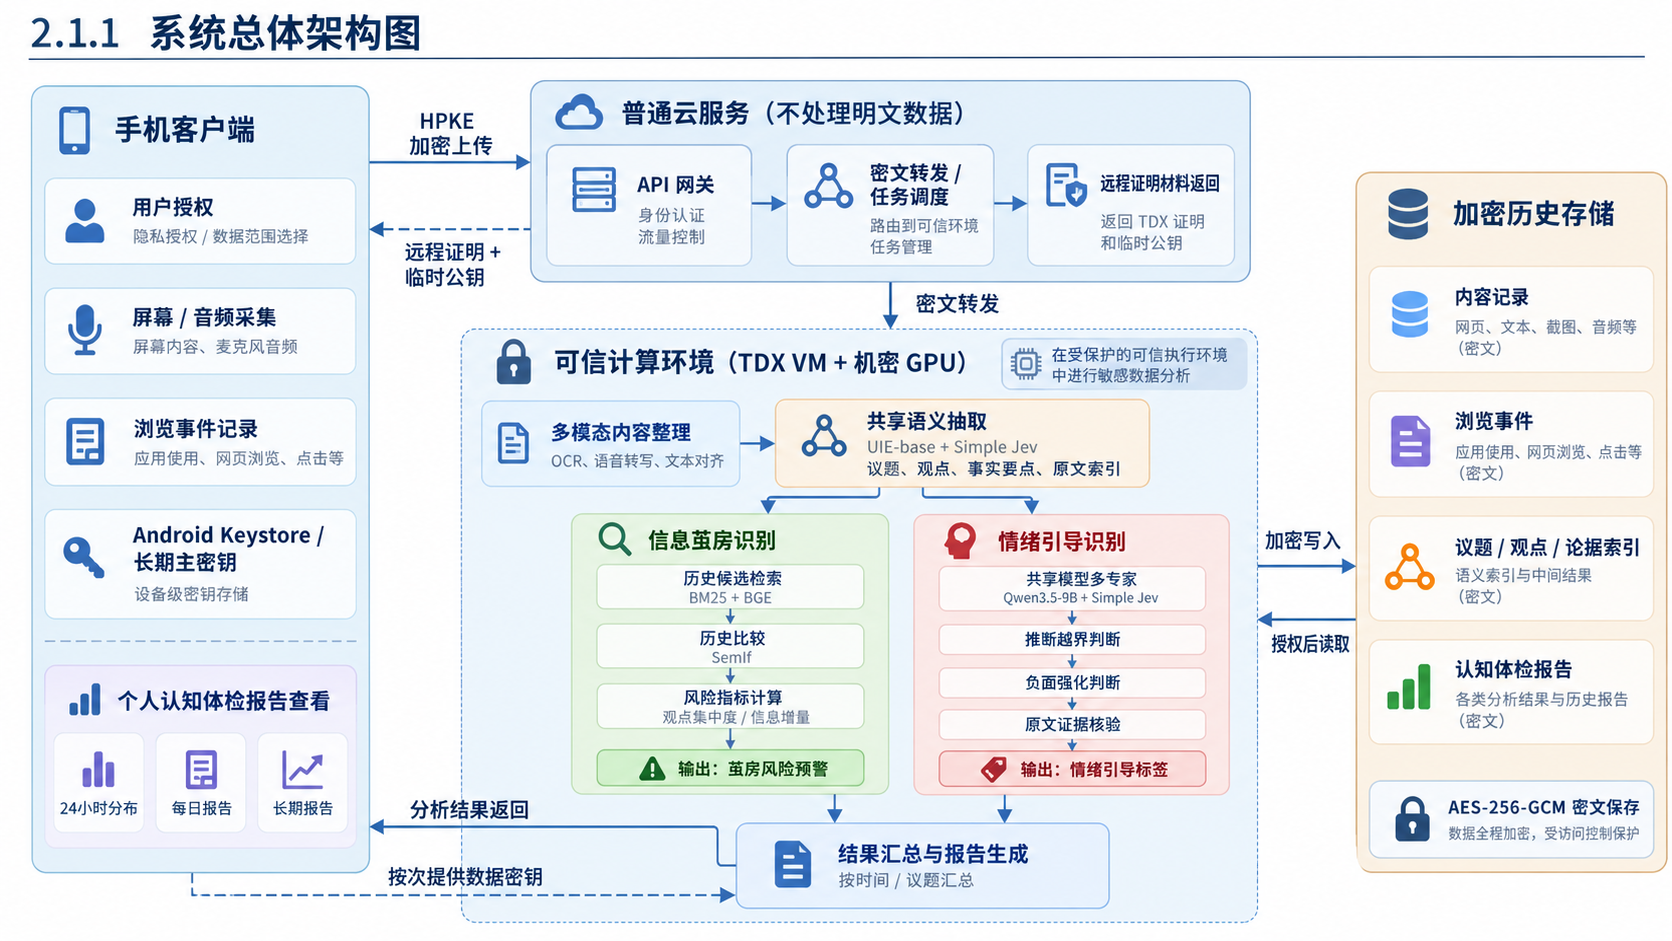
\includegraphics[width=\linewidth,height=0.72\textheight,keepaspectratio]{figures/chapter2/fig_2_1_system_architecture.png}
\caption{可信计算环境系统总体架构图}\label{fig:2-1}
\end{figure}

\subsubsection{多模态浏览内容采集与统一记录}\label{section:2.1.2}

网页、图文帖子和短视频的信息承载方式不同，同一观点可能出现在页面正文、视频字幕或口播中。若只采集某一种文本来源，便可能遗漏用户真正接触的事实与结论。针对这一问题，手机客户端在用户授权后通过Android MediaProjection获取屏幕内容，按照采样与区域裁剪规则保留可观察的信息，并在系统许可的条件下采集音频。同时记录相关内容的接触时间和有效浏览时长，为后续统计提供行为依据。

采集到的画面和音频经加密送入经过验证的可信计算环境，在其中完成OCR识别、语音转写以及文本顺序整理。系统依据页面结构、时间戳和可识别的内容来源，将文字、字幕与口播整理为具有上下文关系的文本片段，合并重复表达，并保留原文位置。这样，后续模型既能获得完整的语境，也能把识别结果追溯到具体页面区域、语句或视频时间点。

在数据组织上，系统区分\textbf{内容记录}与\textbf{浏览事件}。内容记录保存某条内容的可分析文本、来源和原文索引；浏览事件保存用户每次接触该内容的时间及有效停留信息。同一内容未发生变化而被反复观看时，系统可以复用既有的内容解析结果，但仍分别记录每次接触。由此，观点与论据分析以内容为对象，出现频率和浏览时长统计以事件为对象，避免把同一内容的重复观看误认为不同事实，也避免遗漏重复接触本身所反映的信息环境特征。

\subsubsection{共享语义抽取与双路径认知分析}\label{section:2.1.3}

完成多模态文本整理后，系统首先需要回答一条内容究竟讨论了什么问题，表达了哪些判断，以及使用了什么事实加以支持。只有将这些内容转化为稳定的语义记录，才能比较不同视频之间的信息差异，也才能检查负面结论是否超出了原有事实。为此，系统采用2.2节提出的轻量化观点论据提取方法：通过UIE-base定位议题、观点、事实片段及限定条件，再由基于Qwen3.5-0.8B的Simple Jev判别表达类型和观点---论据关系，并将复合论据整理为可独立比较的事实要点。提取结果保留原文位置，供后续两条分析路径共同使用。

\textbf{第一条路径面向信息茧房识别，重点判断当前内容相对于个人历史增加了什么。} 系统利用BM25与BGE-small-zh-v1.5检索相近议题及历史语义候选，再由基于Qwen3.5-4B的SemIf判断议题归属、观点关系和事实等价性。在确定所属议题后，当前论据与该议题下的历史事实要点进行比较，综合不同历史记录的覆盖情况，识别已出现的依据和新增信息。系统进一步按照议题及时间窗口计算观点集中度、有效观点数量、去重论据数量和信息增量率，在有效记录达到要求后，考察主导观点持续集中且新增依据持续不足的情况，并将相关浏览记录作为风险预警的依据。

\textbf{第二条路径面向过度推断型情绪引导识别，重点判断内容如何从事实推导出负面结论。} 系统复用前述事实、观点和论证关系，以整条内容为上下文、以具体评价性结论为判别单元。基于Qwen3.5-9B与Simple Jev的共享模型多专家方法，分别识别事实适用范围的不合理扩大、结论确定程度的提高，以及灾难化或无助化等负面情绪强化。只有推断越界与负面强化同时成立，且能够通过原文证据核验时，才将相应内容标记为过度推断型情绪引导。随后将识别结果与浏览事件关联，统计此类内容的接触次数和有效浏览时长。

两条路径共享内容解析结果和原文证据索引，但分别回答``是否持续获得新的判断依据''和``所接触的结论是否通过不合理推断强化负面情绪''两个问题。系统将它们的结果按照时间和议题汇总，生成24小时信息分布、每日报告和长期分析报告。用户不仅可以查看不同观点的接触比例、信息增量与情绪引导内容占比，还可以进入具体议题，回顾支持各类观点的已浏览内容及其主要论据。对于观点长期集中或依据持续重复的议题，报告提供风险提醒和信息覆盖局限提示，并保留相关原始来源，供用户进一步核查和补充资料。

\paragraph{端侧脱敏与云端结构化接口协同模式的工程边界}
复赛工程在现有服务端保留兼容路由，并增加端侧脱敏的结构化API协同路径。手机在上传前对手机号、身份证号、电子邮箱及识别到的通知前缀执行本地掩码，携带至多15条历史事实候选；模型单次输出观点、事实覆盖关系、情绪引导证据及信息盲区，程序再检查JSON类型、历史引用、事实计数和连续原文片段。有限候选下的历史覆盖不等同于全量历史穷尽核验，正则掩码也不等同于完全匿名化。

该路径采用固定Ed25519公钥验证应用代码度量声明，以X25519和HKDF-SHA256派生双向AES-256-GCM会话密钥，结合持久化版本、哈希及手机检查点检查状态连续性。这是应用层身份与完整性机制，不构成下文硬件TEE远程证明的等价实现。服务进程及所调用的商业模型能够处理脱敏明文，不能据此宣称云端全程不可见明文。本文原有本地模型与硬件隔离设计作为研究方案保留，其实验结论不直接迁移为此API路径的准确率、时延或机密性结论；新增路径的现场可用性需单独验收。

\subsubsection{高频处理与长期历史维护}\label{section:2.1.4}

短视频信息流的内容切换频繁，若每出现一条新内容都由大模型生成完整解释，再逐项扫描全部历史记录，分析任务便容易积压，影响连续体检的使用体验。破茧因此将高频处理拆分为\textbf{片段定位、固定类别判断、历史候选检索和指标计算}四类任务，让不同计算需求由适合的技术承担。

在当前内容处理阶段，UIE-base负责定位语义片段，Simple Jev通过候选类别评分完成结构化判断，减少长文本生成；情绪引导识别中的三个专家共享Qwen3.5-9B的内容上下文，降低重复输入带来的推理开销。在历史比较阶段，BM25与语义检索先缩小候选范围，SemIf只针对相关议题、观点和论据执行关系判别；观点分布、信息新颖度与风险条件则由确定性程序计算。对于内容未发生变化的重复接触，系统复用相应的抽取与判别结果，只为新的浏览事件增加接触记录。

计算提速还必须与历史结果的正确性相协调。不同内容的OCR、文本整理和初步语义抽取可以独立处理；同一用户的历史覆盖判断与语义状态更新则按照实际浏览顺序执行，或依据明确的历史版本完成计算。随着新内容增加，系统按议题持续维护观点簇、事实要点和检索索引；当后续比较确认两个议题或观点簇需要合并时，同步修正历史关联，并重新计算受影响的增量与统计结果。这样，系统能够利用并行处理和历史结果复用适应高频浏览需求，同时保持长期分析口径的一致性。

\subsubsection{贯穿全过程的隐私保护机制}\label{section:2.1.5}

持续认知体检必须长期比较用户浏览历史，而议题、观点、论据和情绪统计等记录本身也可能揭示个人关注的敏感问题。即使原始截图不作长期保存，如果历史索引或分析报告能够被普通服务器管理者读取，仍会带来隐私泄露风险。因此，破茧按照2.4节提出的可验证异构机密计算方案，围绕\textbf{采集端程序可信、上传对象可信、运行中明文受保护、历史解密权由用户控制}建立连续防护链路。

在手机端，系统通过公开安全关键代码、可复现构建及发布版本审核约束采集与对外通信行为。上传数据之前，客户端核验云端Intel TDX可信虚拟机、NVIDIA机密GPU及已批准程序版本的远程证明，并检查本次接收公钥与证明的绑定关系。核验通过后，手机才使用HPKE加密提交数据；普通业务网关仅负责转发密文。真正的解密发生在受保护的CPU内存中，随后的OCR、语音转写、语义模型推理及历史比较均位于经过验证的可信计算边界内，涉及GPU的处理使用受保护的显存与通信链路。

对于需要长期保存的浏览事件、语义索引和认知体检报告，系统使用AES-256-GCM加密存储，并将长期主密钥保留在受Android Keystore保护的手机端。每次需要读取个人历史时，客户端重新验证可信程序，只按次交付本次所需的数据密钥；可信程序在内部完成解密、分析、更新及重新加密，并通过历史版本标识检查状态连续性。分析报告以密文形式保存，或经受保护会话返回手机供用户查看。由此，普通服务器能够管理任务和密文存储，却不能仅凭运维权限获得浏览原文或长期分析结果的解密权。

通过上述设计，破茧形成以真实浏览事件为入口、以观点论据记录为共同基础、以长期历史比较和情绪引导判别为核心的认知体检系统。2.2节进一步介绍观点与论据增量识别及信息茧房风险判定，2.3节介绍共享模型多专家情绪引导识别，2.4节说明各处理阶段如何在可验证的可信计算条件下保护个人隐私。

\subsection{基于观点与论据历史增量的信息茧房识别方法}\label{section:2.2}

\subsubsection{研究问题与总体技术思路}\label{section:2.2.1}

仅凭用户浏览主题的集中程度，无法准确判断其是否陷入信息茧房。例如两名用户都在关注就业形势：一人持续阅读不同地区的招聘数据、行业报告和相互补充的分析；另一人则反复看到不同账号转述同一份报告，并不断重复阅读着相似的结论。两者的浏览主题同样集中，前者不断获得新的判断依据，后者接触的内容虽然数量增加，实际提供的信息却变化有限。因此，识别信息茧房需要考察同一\textbf{议题下的观点是否趋于单一，以及支撑这些观点的论据是否缺乏增量。}

针对这一问题，破茧采用\textbf{基于轻量化信息抽取的观点增量识别方法}。系统首先从用户实际浏览的网页、短视频和评论中提取议题、观点及其论据，再将当前语义内容与个人历史记录比较，识别重复依据和新增事实，最后依据一段时间内的观点分布与论据增量判断信息茧房风险。

为适应连续浏览场景中的高频分析需求，系统将原本由生成式大模型承担的语义处理拆分为两个阶段。在当前内容分析阶段，采用UIE-base定位观点与事实片段，利用基于Qwen3.5-0.8B的Simple Jev进行表达类型和论证关系判别；在历史比较阶段，利用BM25与BGE-small-zh-v1.5召回相关议题及历史语义候选，再由基于Qwen3.5-4B的SemIf完成议题匹配、观点归并与论据关系判别。两套本地决策框架均直接对预设选项评分，以降低单次判别的生成开销。事实覆盖、窗口指标和长期风险则由确定性程序计算，形成从当前内容理解到历史增量分析的连续处理链路。

流程图如图所示（后续改）：

\begin{figure}[htbp]
\centering
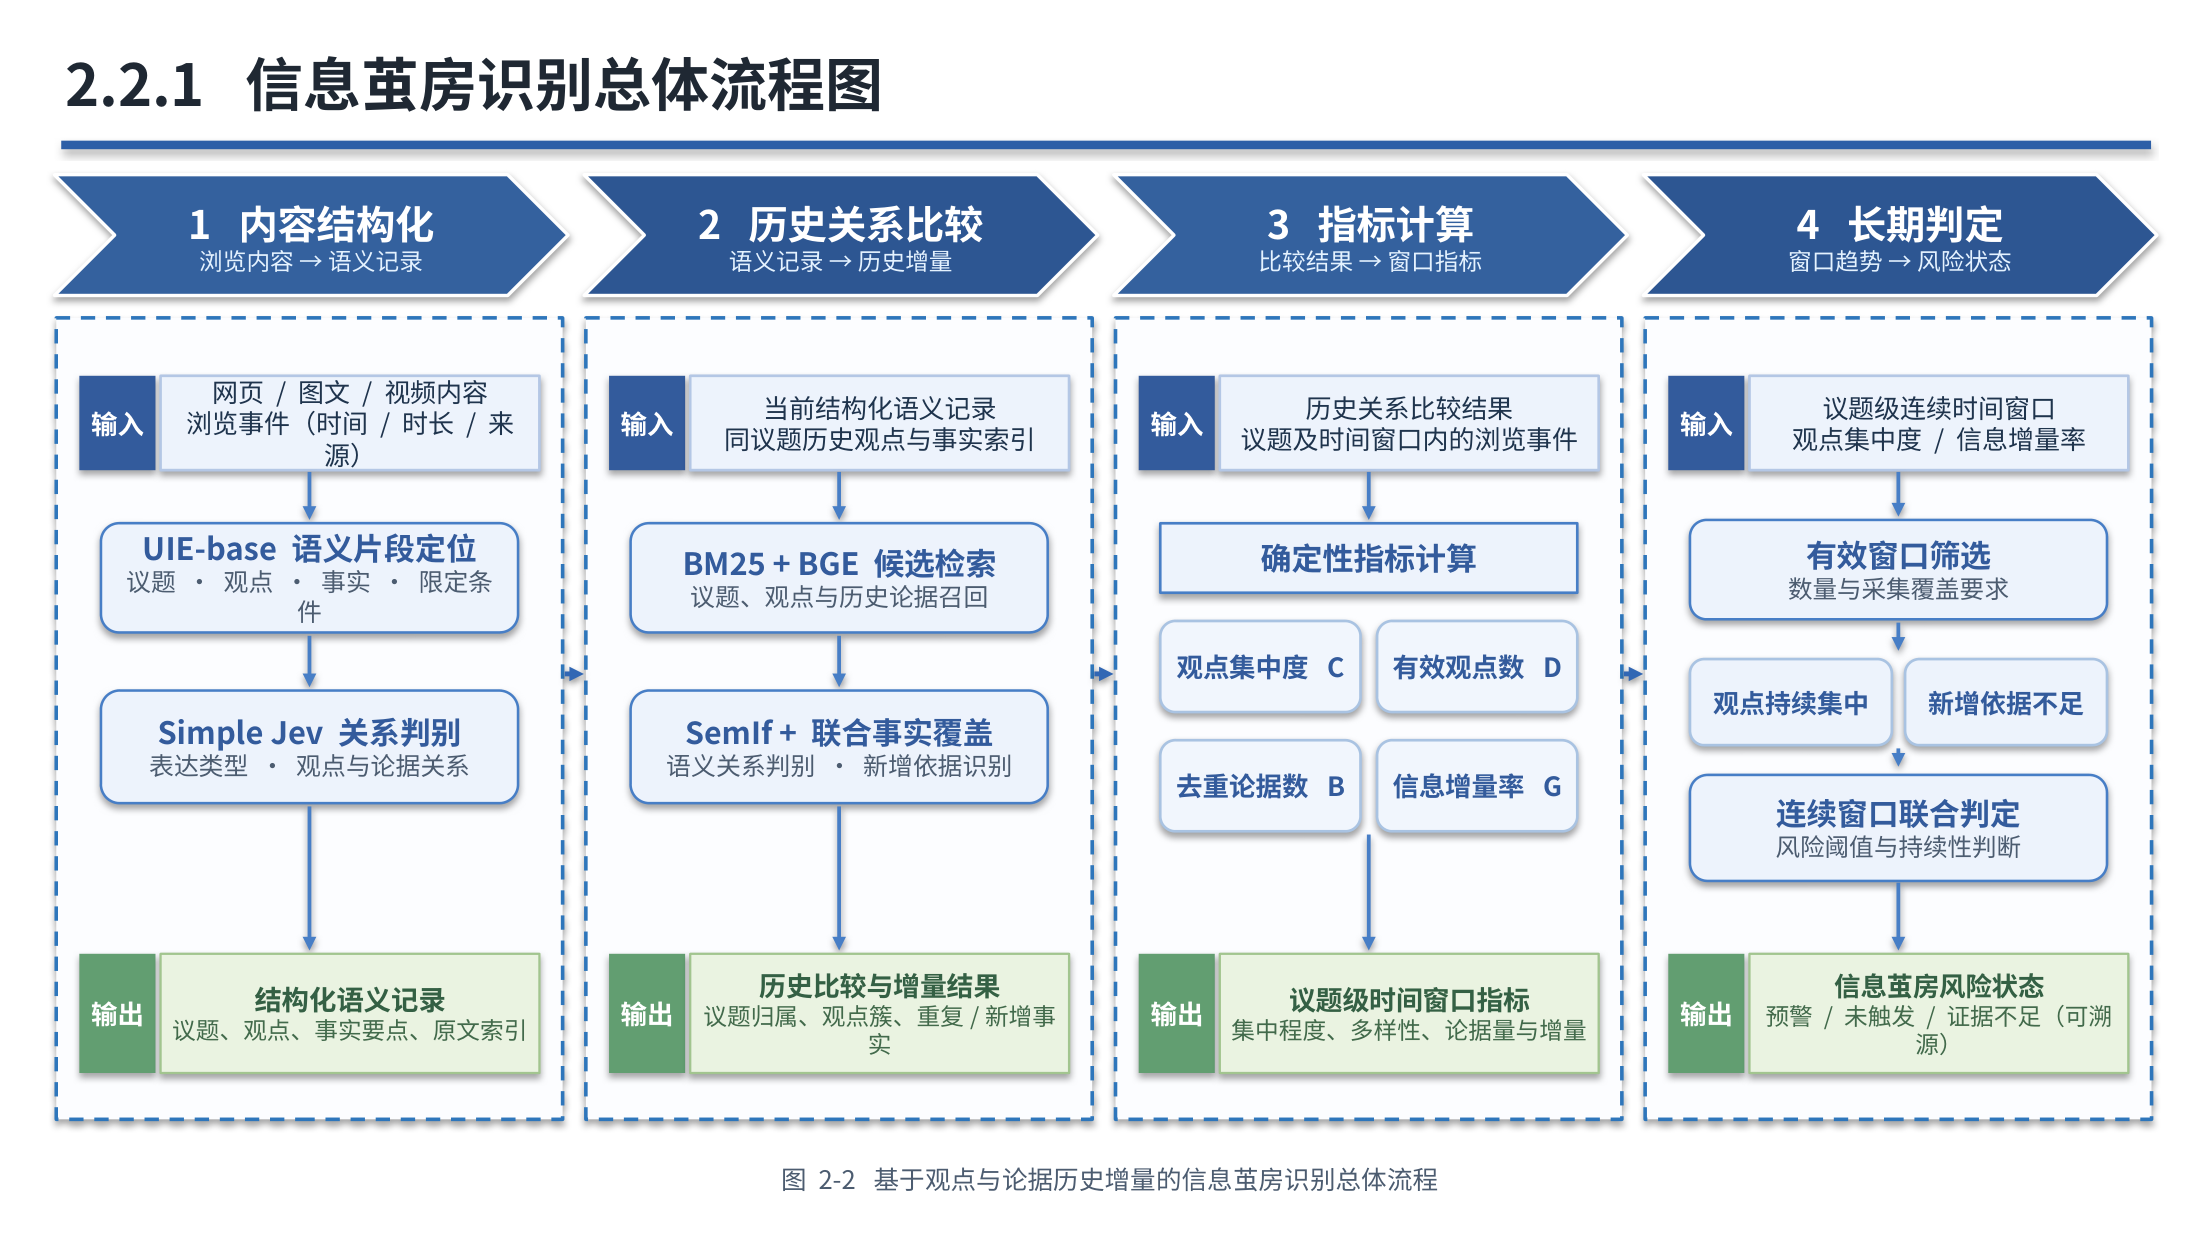
\includegraphics[width=\linewidth,height=0.72\textheight,keepaspectratio]{figures/chapter2/fig_2_2_cocoon_detection.png}
\caption{信息茧房识别总体流程图}\label{fig:2-2}
\end{figure}

\subsubsection{基于UIE与本地结构化决策的观点论据提取}\label{section:2.2.2}

判断信息是否重复，首先要明确一条内容实际表达了什么观点，又使用了哪些依据。网络文章和短视频常将事实、个人经历和主观判断交织在一起，同一段话还可能讨论多个问题。若直接比较整段内容，容易将观点相近但依据不同的材料判为重复，也可能忽略不同表达中反复引用的同一事实。因此，系统先定位原文中的语义片段，再识别片段类型及其论证关系。

系统将接收采集模块收集到的网页文字、OCR识别结果和语音转写文本，依据页面结构、时间戳和来源标识恢复可观察内容的顺序。预处理合并字幕与画面文字中的重复内容，按句子和段落组织文本，并保留必要的相邻上下文。对于较长的文章和视频，采用带重叠上下文的分段方式，每个片段均保存内容标识、原文位置、接触时间和可识别的表达主体，使后续抽取结果能够追溯到用户实际接触的内容。

在片段定位阶段，系统采用通用信息抽取模型UIE-base，按照预设的抽取模式识别议题表述、判断性语句、事实性片段，以及时间、地区、人群等限定条件。\textbf{观点}指针对某一问题提出的判断，例如``应届生求职竞争正在加剧''；\textbf{论据}指内容为支持或反驳某种判断而引用的事实、数据、案例或解释，例如``某地区互联网行业招聘岗位同比减少20\%''。UIE返回候选片段及其原文位置，为后续判断提供明确的文本对象。

语句片段在论证中的作用，需要结合上下文进一步判断。例如，文章可能先引用``就业形势正在好转''的说法，再提出反对意见；一项招聘数据也可能被作者用于支持多个判断。因此，系统将UIE提取的候选片段及局部上下文输入本地Simple Jev，由Qwen3.5-0.8B对预定义问题进行结构化决策。模型首先区分事实陈述、观点表达与引用内容，再针对候选观点---论据组合判断其关系属于支持、反驳、无关或不确定，并结合上下文确定表达主体。对于同一片段涉及的多个判别问题，采用共享上下文的批量决策方式返回类别及相应分值。

为支持后续的信息增量计算，系统进一步把包含多项独立事实的论据划分为事实要点。具体做法是利用句法边界、并列连接和UIE定位结果生成候选要点，再由Simple Jev判断其是否具有相对完整的事实含义，并确认主体、时间和适用范围。这样，一条同时讨论``招聘岗位减少''和``应聘人数增加''的论据可以保留两个独立要点。对于跨句表达，系统结合重叠上下文检查要点与原文的对应关系。

整理后的结果通过原文位置校验和字段一致性检查，写入统一的语义记录。对于第\(i\)次浏览涉及的议题\(q\)，记为\(z_i^q=(\mathcal V_i^q,\mathcal E_i^q,\mathcal R_i^q)\)，其中\(\mathcal V_i^q\)为观点集合，\(\mathcal E_i^q\)为带有事实条件和要点信息的论据集合，\(\mathcal R_i^q\)为观点与论据之间的论证关系。每项记录均保留原始来源和表达主体，作为后续历史比较及主题观点整理的共同输入。

\subsubsection{基于SemIf的历史语义比较与信息增量识别}\label{section:2.2.3}

一项事实是否属于新增信息，取决于用户此前已经接触过什么。系统将第\(i\)次接触记录为浏览事件\(b_i=(x_i,t_i,d_i)\)，分别表示浏览内容、接触时间和有效接触时长，并按议题维护历史观点与论据索引。新内容完成结构化提取后，依据实际浏览顺序与此前的历史进行比较，再写入本次记录。对于重复观看，系统复用已有的片段提取结果，同时保留新的接触事件，使内容计算与实际接触次数相互区分。

\begin{figure}[htbp]
\centering
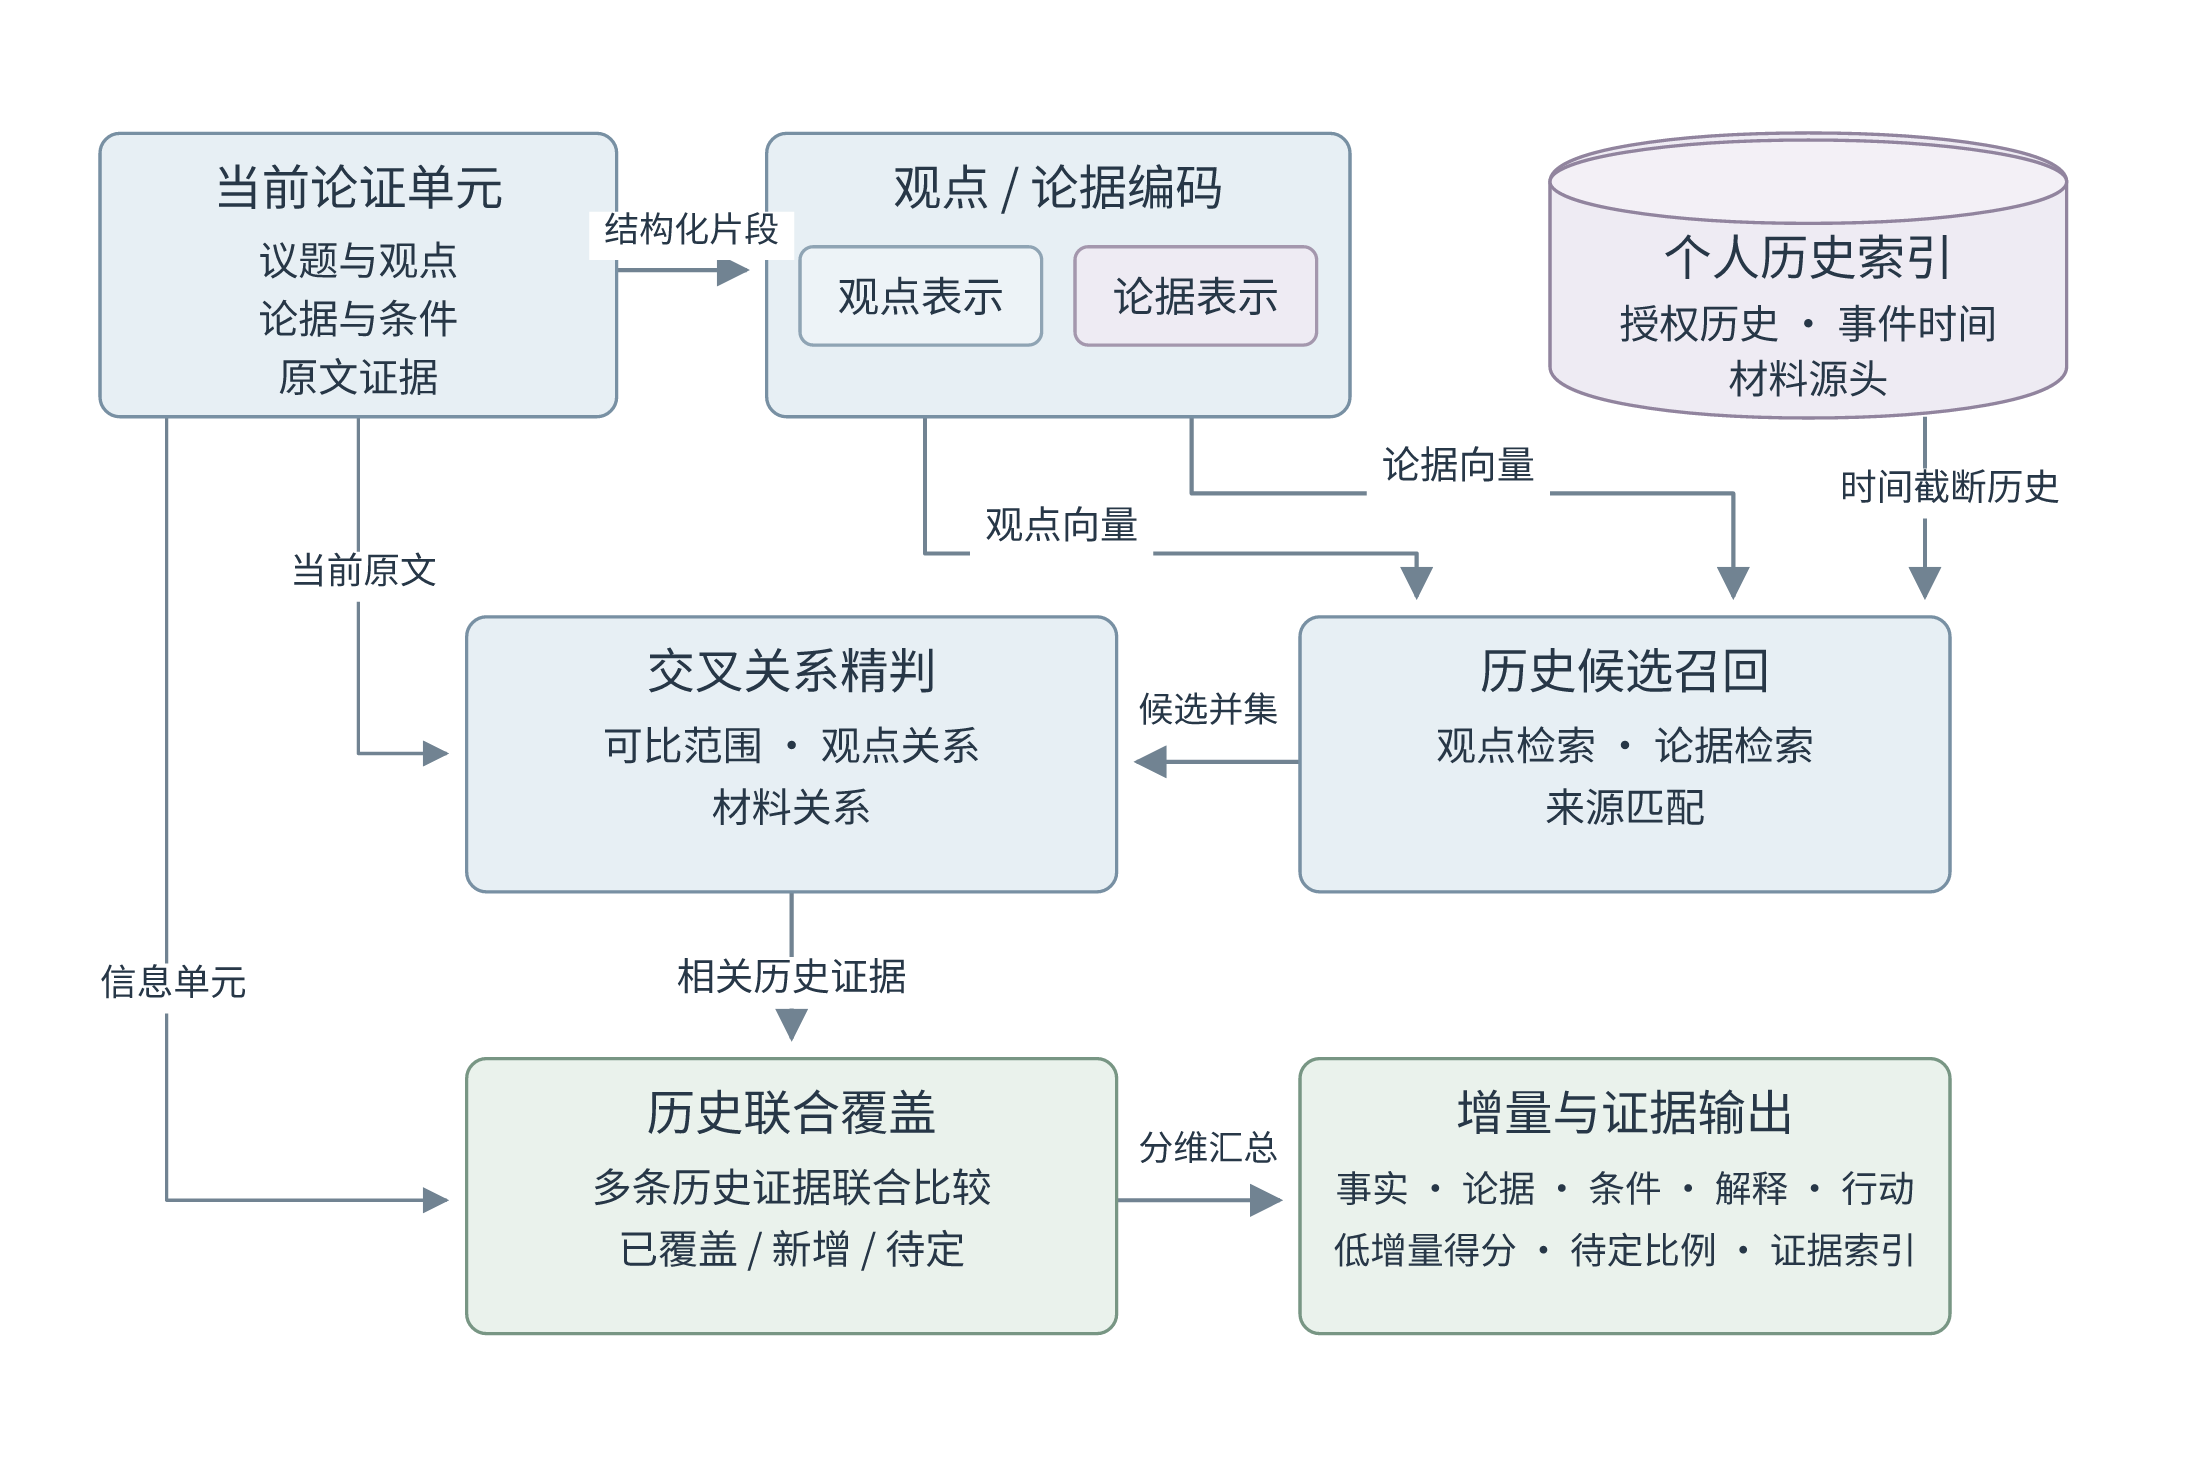
\includegraphics[width=\linewidth,height=0.72\textheight,keepaspectratio]{figures/chapter2/fig_2_3_history_increment.png}
\caption{分级匹配与历史更新流程图}\label{fig:2-3}
\end{figure}

在历史比较之前，系统先确定当前内容所属的议题。对于UIE提取的议题表述，利用BM25与BGE-small-zh-v1.5分别从词项和语义层面召回个人历史中的相近议题，再由SemIf判定同一议题、上下位相关或不同议题。判定为同一议题的内容归入已有档案，上下位议题保留关联；无法归入已有档案的内容建立新议题，并初始化观点簇与论据索引。

确定议题归属后，系统使用\textbf{观点与论据双路候选检索}：观点检索关注讨论对象与判断方向，结合BM25与BGE-small-zh-v1.5召回相近观点；论据检索关注事实主体、数据和适用条件，利用BM25召回候选，再依据结构化字段筛选和排序。由此将针对全部历史的比较，转化为当前语义单元与少量候选之间的关系判别。

对于检索得到的候选，系统采用\textbf{基于SemIf的本地语义关系决策方法}。SemIf以当前观点或论据、候选历史片段及其事实条件为共同输入，利用Qwen3.5-4B直接读取预设关系选项的模型分值。观点比较区分语义相近、相互反驳及不同判断；论据比较区分事实等价、部分重合、不同事实及无法确定，并重点检查主体、时间、地区等限定条件是否一致。对于同一当前语义单元召回的多项候选，复用共同输入上下文进行多项关系判断。

根据观点关系判别结果，系统将判断对象、方向及适用条件一致的观点归入已有簇，对无法归并的观点建立新簇，并保留不同观点簇之间的反驳关系。新议题和观点簇的展示名称优先采用UIE抽取的原文表述；缺少适合展示的名称时，复用Qwen3.5-4B的常规文本生成接口生成简明名称。议题和观点簇使用稳定标识存储，名称用于浏览报告中的展示。

单项候选比较仍无法完整反映历史信息的覆盖情况。一条新视频可能重新组合此前多条视频提供的事实，虽然没有任何一条历史材料与之完全一致，其中的事实却可能都已出现。因此，系统采用\textbf{基于事实要点的历史证据联合覆盖方法}：以2.2.2节形成的事实要点为单位，汇总来自不同历史记录的SemIf判别结果。只有当历史材料能够覆盖某一要点的事实内容及必要限定条件时，才将该要点认定为已出现；多个要点可以分别由不同历史来源覆盖。

设当前论据\(e\)包含\(J_e\)个事实要点，第\(j\)个要点的历史覆盖标记为\(c_j\)，已覆盖取1、新增取0。其历史覆盖程度定义为：

\begin{equation}
\operatorname{Cov}(e,\mathcal H_q^{<i})=\frac{\sum_{j=1}^{J_e}\omega_jc_j}{\sum_{j=1}^{J_e}\omega_j},\qquad c_j\in\{0,1\}
\label{eq:2-1}
\end{equation}

其中，\(\mathcal H_q^{<i}\)表示本次浏览发生前的同议题历史记录，\(\omega_j\)为事实要点权重，初始采用等权计算。在此基础上，定义当前论据相对于个人历史的信息新颖度：

\begin{equation}
\nu(e,\mathcal H_q^{<i})=1-\operatorname{Cov}(e,\mathcal H_q^{<i})
\label{eq:2-2}
\end{equation}

对于首次出现的议题，\(\mathcal H_q^{<i}\)为空，已识别的有效事实要点均计为新增；对于已有议题中新建的观点簇，论据仍与该议题的全部历史记录进行比较。

例如，一条视频同时提到``招聘岗位减少''\,``应聘人数增加''和一项新的毕业生调查结果。前两项分别出现在用户此前浏览过的不同视频中，第三项为首次接触的事实。在三个要点等权时，该论据的信息新颖度为\(1/3\)。系统保存每项覆盖判断所对应的历史片段和原始来源；对于尚不能确认覆盖关系的论据，先保留待核验状态，确认后再纳入有效增量统计。

随着浏览记录增加，系统复用候选检索与SemIf机制复核可能重合的议题和观点簇。确认属于同一议题或同一观点的簇进行合并，保留旧簇标识到目标簇的映射，并更新浏览事件关联及历史检索索引。对于议题归属发生变化的记录，按原始浏览顺序重新计算受影响的历史事实覆盖与窗口指标；观点簇合并则同步更新观点分布指标和相关风险结果。原文片段及其来源记录继续保留，供后续追溯。

由于不同内容的抽取可以独立执行，系统允许新浏览内容并行完成UIE与Simple Jev处理；涉及个人历史的语义比较和状态更新则按照浏览事件的实际顺序执行，或基于相应的历史版本进行计算。这样既能减少前端浏览对后台分析的等待，也能保证信息新颖度始终相对于正确的先前历史定义。

\subsubsection{观点分布与信息增量指标计算}\label{section:2.2.4}

完成观点归并和历史比较后，系统以\textbf{议题\(q\)和时间窗口\(W\)}为统计单位，将分散的浏览记录转化为四项指标。设\(\mathcal B_q(W)\)为窗口内与议题\(q\)相关的有效浏览事件集合，\(K_q\)为该窗口出现的观点簇数量。同一浏览事件对同一观点簇计一次，一条内容涉及不同观点时分别记录。四项指标分别反映观点接触的集中程度、分布多样性、依据数量和历史增量。

\textbf{（1）观点集中度。} 为衡量用户是否主要接触某一种判断，先计算第\(k\)个观点簇在窗口内的接触比例：

\begin{equation}
p_{qk}(W)=\frac{n_{qk}(W)}{\sum_{j=1}^{K_q}n_{qj}(W)}
\label{eq:2-3}
\end{equation}

其中，\(n_{qk}(W)\)为关联该观点簇的有效浏览事件数。在此基础上，以占比最高的观点衡量集中程度：

\begin{equation}
C_q(W)=\max_{1\leq k\leq K_q}p_{qk}(W)
\label{eq:2-4}
\end{equation}

\(C_q(W)\)越高，说明用户接触的内容越集中于某一主导观点。例如，围绕就业形势的有效观点接触中，若80\%表达``形势趋于严峻''，则观点集中度为0.8。

\textbf{（2）有效观点数量。} 观点集中度反映主导观点的优势。系统进一步采用基于信息熵的有效观点数量，刻画不同观点的整体分布：

\begin{equation}
D_q(W)=\exp\left(-\sum_{k=1}^{K_q}p_{qk}(W)\ln p_{qk}(W)\right)
\label{eq:2-5}
\end{equation}

当所有接触都集中于一个观点时，该指标为1；当多个观点的接触份额更加均衡时，指标相应增大。该指标与观点集中度共同呈现用户所接触观点的结构。

\textbf{（3）去重论据数量。} 同一事实可能被不同账号反复引用，仅统计论据出现次数会高估信息丰富度。系统依据SemIf得到的历史语义关系，对事实内容及适用条件一致的论据进行归并，计算窗口内实际涉及的不同依据数量：

\begin{equation}
B_q(W)=\left|\operatorname{Dedup}(\mathcal E_q(W))\right|
\label{eq:2-6}
\end{equation}

其中，\(\mathcal E_q(W)\)为窗口内的论据出现记录，\(\operatorname{Dedup}\)表示基于语义等价与事实条件的去重操作。例如，十条视频均引用同一项招聘调查时，该调查计为一项去重论据，各视频的出现次数与来源仍分别保留。

\textbf{（4）信息增量率。} 去重论据数量反映窗口内接触了多少种不同依据，信息增量率进一步衡量这些依据相对于此前历史增加了多少内容。设\(\mathcal E_{i,\mathrm{valid}}^q\)为第\(i\)次浏览中已完成历史覆盖判断的论据集合，则窗口信息增量率定义为：

\begin{equation}
G_q(W)=\frac{\displaystyle\sum_{b_i\in\mathcal B_q(W)}\sum_{e\in\mathcal E_{i,\mathrm{valid}}^q}\nu(e,\mathcal H_q^{<i})}{\displaystyle\sum_{b_i\in\mathcal B_q(W)}|\mathcal E_{i,\mathrm{valid}}^q|}
\label{eq:2-7}
\end{equation}

\(G_q(W)\)表示窗口内有效论据信息新颖度的平均值。数值较低说明当前浏览内容较多复用了已接触的事实，数值较高则说明用户持续获得新的判断依据。该指标与观点集中度结合，可以区分``观点相近但论据持续增加''和``观点相近且依据长期重复''两种不同的信息接触模式。没有有效论据的窗口不计算信息增量率，也不计入需要该指标的有效风险判定窗口。

\subsubsection{基于长期浏览记录的信息茧房风险判定}\label{section:2.2.5}

判断信息茧房的长期风险，需要考察观点集中与依据重复的持续性。例如，用户为准备求职面试连续观看多条相关视频，可能暂时形成较高的观点集中度。因此，系统按日或设定时长汇总观点分布与信息增量，重点考察\textbf{主导观点持续集中、同时新增论据持续不足}的接触模式。

设\(W_t\)为第\(t\)个时间窗口。当观点集中度达到阈值\(\theta_C\)，且信息增量率低于阈值\(\theta_G\)时，定义该窗口满足联合条件：

\begin{equation}
A_q(W_t)=\mathbb I\left[C_q(W_t)\geq\theta_C\ \land\ G_q(W_t)\leq\theta_G\right]
\label{eq:2-8}
\end{equation}

系统进一步记录联合条件连续成立的窗口数量。设\(U_q(W_t)\)为窗口有效性标记，\(\ell_q(t)\)为截至第\(t\)个窗口的连续长度，其更新规则为：

\begin{equation}
\ell_q(t)=\begin{cases}\ell_q(t-1)+1,&U_q(W_t)=1\ \land\ A_q(W_t)=1,\\0,&\text{其他情况。}\end{cases}\qquad \ell_q(0)=0
\label{eq:2-9}
\end{equation}

窗口有效性依据可用浏览数量、采集覆盖和已完成的语义分析结果确定。设观察期内的最大连续长度为\(L_q(T)=\max_{1\leq t\leq T}\ell_q(t)\)，有效窗口数量为\(n_q^{\mathrm{valid}}(T)\)。当有效记录达到最低数量要求，且联合条件持续达到设定长度时，系统输出信息茧房风险预警：

\begin{equation}
R_q(T)=\begin{cases}\bot,&n_q^{\mathrm{valid}}(T)<n_{\min},\\1,&L_q(T)\geq L_{\min},\\0,&\text{其他情况。}\end{cases}
\label{eq:2-10}
\end{equation}

其中，\(n_{\min}\)为最低有效窗口数，\(L_{\min}\)为持续性阈值；\(R_q(T)\)分别以1、0和\(\bot\)表示触发预警、未触发预警及证据不足。各阈值根据标注数据上的误报和漏报表现确定。预警结果同时关联对应的时间窗口、主导观点、重复论据及原始来源，使用户能够了解风险判断来自哪些实际浏览内容。

通过上述方法，破茧将浏览过程中的零散观点与论据转化为可追溯的长期信息接触特征。UIE与本地快速决策模型承担高频语义处理，SemIf完成个人历史关系判别，确定性程序计算观点结构和事实增量。\textbf{系统据此考察同一议题下观点的持续集中程度，以及支撑这些观点的事实依据是否仍在增加。}

\subsection{基于共享模型多专家判别的情绪引导识别方法}\label{section:2.3}

\subsubsection{研究问题与总体技术思路}\label{section:2.3.1}

在网络平台上，点击数量与用户互动往往直接影响内容的传播效果，部分内容创作者会刻意放大现实问题中的负面因素以博取更多互动与流量，例如通过制造焦虑、恐惧等情绪吸引用户持续评论与转发。这类内容通常并不直接编造虚假信息，而是通过个别的真实事件或有限数据为依据，将局部现象夸大为普遍趋势。例如，某家企业缩减招聘规模是真实事件，但据此断言``就业市场已经全面崩溃，普通人再努力也没有出路''，强化了受众对就业前景的焦虑。由于这类内容往往包含真实的事实依据，其引导性主要体现在从事实到结论的过度推断过程中存在逻辑问题，因此仅依靠虚假信息检测或情绪分类，难以准确识别其中的情绪引导。

针对这一问题，破茧重点识别\textbf{网络内容是否利用有限的事实依据，推导出夸大或绝对化的负面结论，从而强化受众的焦虑、恐惧等情绪}。判断过程需要同时回答三个相互关联的问题：原文提供了什么事实，事实能够支持多大范围的结论，以及评价性表达是否进一步强化了焦虑、恐惧或无助感。只有把这些判断与原文片段联系起来，系统才能给出可核查的情绪引导识别结果。

为完成这一判断，系统还需要解决网络内容中事实与结论分散的问题。一条短视频可能先介绍局部事件，再穿插其他材料，最后给出面向整体形势的评价；同一条内容也可能包含多个不同的结论。孤立分析某一句话，难以准确判断它与前文事实的关系。为此，系统复用2.2节抽取的事实、观点及论证关系，以\textbf{整条内容为分析上下文，以具体评价性结论为判别单元}，分别检验每项结论与其相关依据之间的关系。

日常信息流还具有内容出现频繁、浏览间隔短的特点。针对这一需求，破茧采用\textbf{Qwen3.5-9B与Simple Jev相结合的共享模型多专家判别方法}：由同一语言模型承担三个维度的语义判断，利用Simple Jev替代传统的LLM技术来加速该分析过程，先在共享上下文上完成预设类别的候选评分，然后再通过逻辑规则融合各项判断，最后在生成报告时利用2.2节保留的原文索引来还原原文内容。由此，系统将复杂的情绪引导分析转化为可复用的结构化判别过程，为连续浏览场景下的内容识别和接触统计提供基础。

\begin{figure}[htbp]
\centering
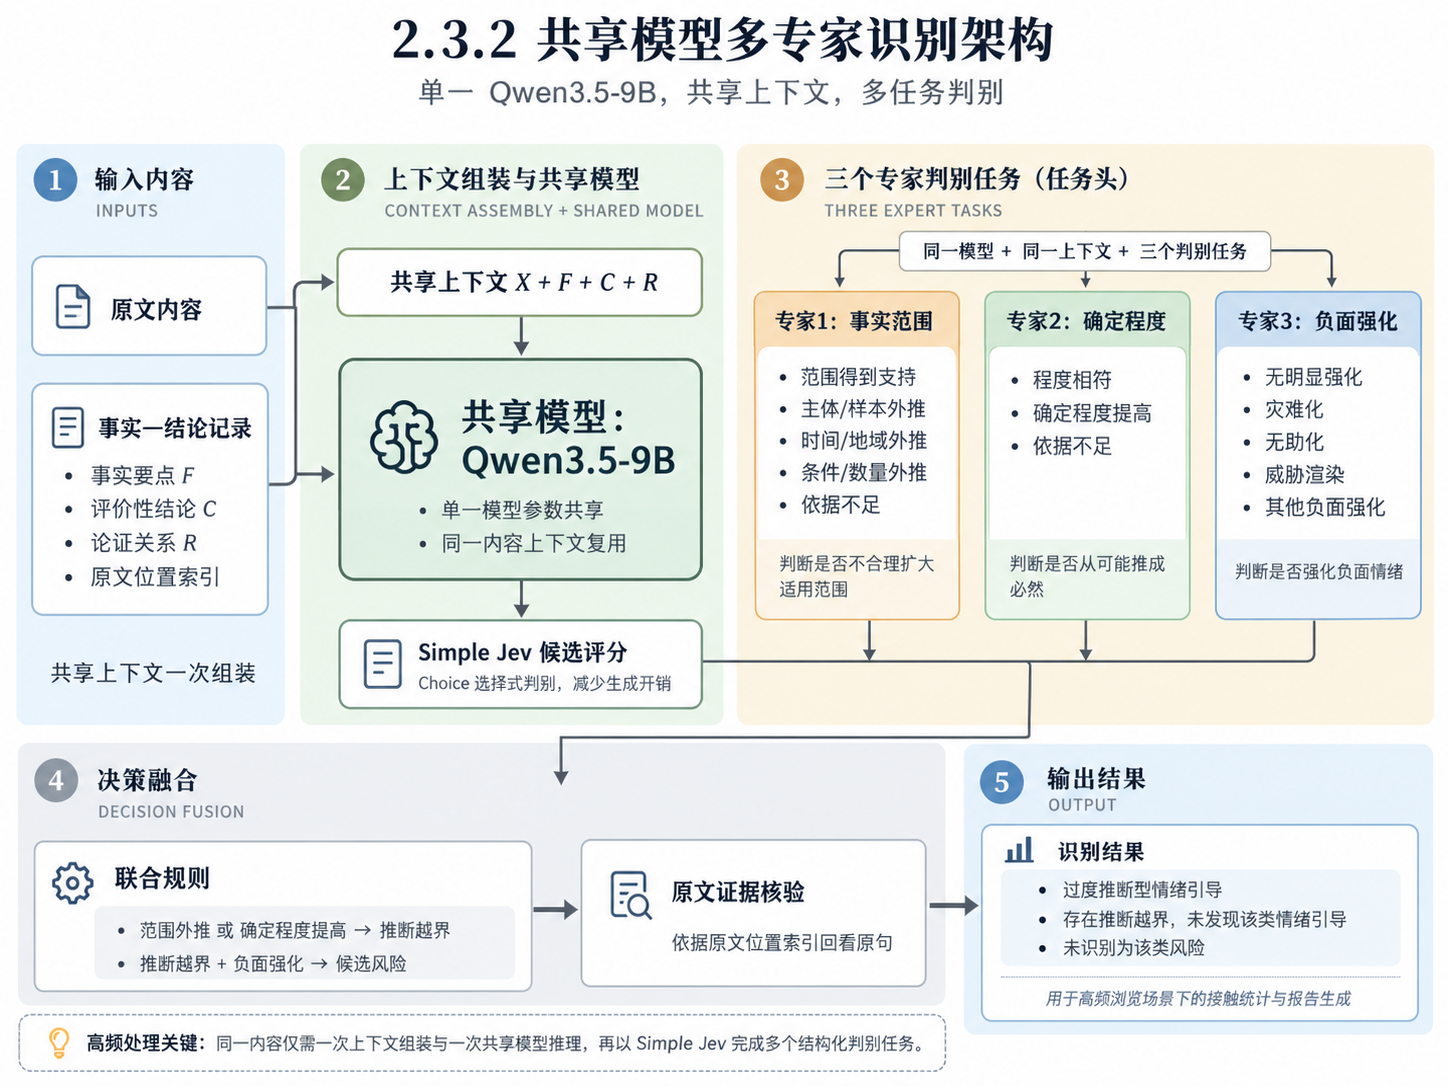
\includegraphics[width=\linewidth,height=0.72\textheight,keepaspectratio]{figures/chapter2/fig_2_4_emotional_guidance.png}
\caption{共享模型多专家识别架构流程图}\label{fig:2-4}
\end{figure}

\subsubsection{基于共享上下文的多专家语义判别}\label{section:2.3.2}

事实外推、确定性提高与负面情绪强化虽然可能同时出现在同一段表述中，但各自对应不同的判断标准。例如，``部分岗位减少''被推及``所有行业''属于事实适用范围的扩大；``岗位可能减少''被改写为``必然失业''则属于结论确定程度的提高。只有将这些差异区分开来，才能说明一条内容的引导性具体来自何处。

据此，系统在Qwen3.5-9B上设置事实范围、确定程度和情绪表达三个语义判别专家。三个专家共享模型参数和内容上下文，分别采用独立的判别问题与候选类别。其中，事实范围专家综合相关事实及其限定条件，识别结论对主体、时间、地域或适用条件的不合理外推；确定程度专家比较事实依据与结论的判断强度，识别从可能、局部到必然、普遍的推断变化；情绪表达专家结合语境，识别灾难化、无助化和威胁渲染等负面强化方式。具体分类设置如下表所示。

\begingroup
\small
\begin{longtable}{@{}
>{\RaggedRight\arraybackslash}p{(\linewidth - 4\tabcolsep) * \real{0.1600}}
>{\RaggedRight\arraybackslash}p{(\linewidth - 4\tabcolsep) * \real{0.2800}}
>{\RaggedRight\arraybackslash}p{(\linewidth - 4\tabcolsep) * \real{0.5600}}@{}}
\caption{三个语义判别专家的分类任务与候选类别}\label{tab:2-2}\tabularnewline
\toprule
判别专家 & 核心判断 & 候选类别 \\
\midrule
\endfirsthead
\toprule
判别专家 & 核心判断 & 候选类别 \\
\midrule
\endhead
\bottomrule
\endlastfoot
事实范围专家 & 结论的适用范围是否获得事实支持 & 范围得到支持；主体或样本外推；时间或地域外推；数量或条件外推；多维外推；依据不足 \\
确定程度专家 & 结论的确定程度是否超出事实依据 & 程度相符；确定程度提高；依据不足 \\
情绪表达专家 & 结论是否采用负面情绪强化表达 & 无明显强化；灾难化；无助化；威胁渲染；其他负面强化；语境不明 \\
\end{longtable}
\endgroup

对于一条包含多项评价性结论的内容，系统将原始文本与2.2节提取的事实、结论和论证关系组成共享上下文，再以结论编号指定各专家的判断对象。Simple Jev将每项判断组织为具有固定候选类别的Choice问题，利用公共输入的计算结果对候选答案进行评分。与逐项生成自然语言解释相比，这种方式将模型推理集中于类别选择，并减少同一内容在多个判断任务中的重复处理。第\(i\)条内容中第\(j\)项结论的专家判别表示为：

\begin{equation}
\hat y_{ij}^{(k)}=\underset{y\in\mathcal Y_k}{\arg\max}\;P_{\theta}\!\left(y\mid X_i,F_i,C_i,R_i,q_{ij}^{(k)}\right),\quad k\in\{\mathrm{scope},\mathrm{certainty},\mathrm{emotion}\}
\label{eq:2-11}
\end{equation}

其中，\(X_i\)为原始内容上下文，\(F_i\)、\(C_i\)和\(R_i\)分别表示事实集合、评价性结论集合及论证关系；\(q_{ij}^{(k)}\)为第\(k\)个专家针对第\(j\)项结论提出的判别问题，\(\mathcal Y_k\)为相应的候选类别集合。\(P_{\theta}\)表示Qwen3.5-9B经Simple Jev计算的候选类别相对得分分布，\(\hat y_{ij}^{(k)}\)为得分最高的类别。三个专家由此获得结构一致、含义互补的判断结果，为后续联合判定提供依据。

\subsubsection{基于逻辑约束的专家决策融合与原文证据核验}\label{section:2.3.3}

三个专家的输出分别描述推断依据与表达方式，仍需进一步确定它们是否共同构成情绪引导。单纯的负面表达可能只是对事实的合理评价；缺乏依据的外推也未必伴随情绪强化。因此，本模块将\textbf{推断越界与负面情绪强化同时出现}作为过度推断型情绪引导的核心判据，并要求相关判断能够对应到原文依据。

具体而言，事实范围专家识别出不合理外推，或确定程度专家识别出缺乏依据的确定性提高时，判定该结论存在推断越界；在此基础上，若情绪表达专家同时识别出负面强化，并通过原文证据核验，则将其归为过度推断型情绪引导。联合判定规则表示为：

\begin{equation}
G_{ij}=\mathbb I\!\left[(S_{ij}\lor D_{ij})\land E_{ij}\land V_{ij}\right]
\label{eq:2-12}
\end{equation}

其中，\(S_{ij}\)和\(D_{ij}\)分别表示事实范围外推与确定程度提高是否成立，\(E_{ij}\)表示是否存在负面情绪强化，\(V_{ij}\)表示原文证据核验是否通过，\(G_{ij}\)为最终判定结果。各类判断组合及其输出如下表所示。

\begingroup
\small
\begin{longtable}{@{}
>{\RaggedRight\arraybackslash}p{(\linewidth - 6\tabcolsep) * \real{0.3100}}
>{\RaggedRight\arraybackslash}p{(\linewidth - 6\tabcolsep) * \real{0.1600}}
>{\RaggedRight\arraybackslash}p{(\linewidth - 6\tabcolsep) * \real{0.1200}}
>{\RaggedRight\arraybackslash}p{(\linewidth - 6\tabcolsep) * \real{0.4100}}@{}}
\caption{多专家决策融合规则}\label{tab:2-3}\tabularnewline
\toprule
推断越界判断 & 负面情绪强化 & 原文核验 & 最终识别结果 \\
\midrule
\endfirsthead
\toprule
推断越界判断 & 负面情绪强化 & 原文核验 & 最终识别结果 \\
\midrule
\endhead
\bottomrule
\endlastfoot
存在范围外推或确定程度提高 & 存在 & 通过 & 过度推断型情绪引导 \\
存在范围外推或确定程度提高 & 未发现 & 通过 & 存在推断越界，未发现该类情绪引导 \\
未发现推断越界 & 存在 & 通过 & 存在负面情绪强化，未发现该类情绪引导 \\
未发现推断越界 & 未发现 & 通过 & 未发现该类情绪引导特征 \\
\end{longtable}
\endgroup

联合判定能否用于认知体检报告，还取决于判断依据是否真实对应用户接触的内容。为此，系统沿用2.2节保存的事实、结论及论据的原文索引，将专家判断关联到具体语句及其所在语境。对于图文内容，索引指向原始文本位置或OCR文字区域；对于视频内容，索引指向语音转写时间戳或画面文字位置。系统据此核对被引用事实的限定条件、事实与结论的论证关系，以及相关表述究竟属于作者自身判断还是对他人观点的转述。

当原文对应关系明确且各项判断一致时，系统形成包含引导类型、推断变化、情绪强化方式和原文位置的识别记录。对于依据不足、语境不明或存在冲突的情况，系统保留待核验状态，并围绕争议结论追加针对性的Jev分类判断。这样，情绪引导标签不仅具有明确的形成规则，也能落实到具体的事实、结论及其来源，为后续报告中的证据展示提供支持。

\subsubsection{用户接触情绪引导内容的统计与展示}\label{section:2.3.4}

对单条结论的判别只能说明某段内容具有什么表达特征，而认知体检还需要回答用户在日常浏览中实际接触了多少此类信息。为此，系统将结论级判断汇总为内容级结果，再与浏览事件中的接触时间、有效停留时长及所属议题关联。当一条内容包含多项结论时，只要其中一项被确认为过度推断型情绪引导，该内容即获得相应标记；同一次浏览始终作为一条事件统计，以保持内容识别和用户接触行为之间的对应关系。

在此基础上，系统计算情绪引导内容在已完成判定浏览事件中的数量占比，以及其有效浏览时长占比，分别反映用户接触此类内容的频率和注意力投入。进一步按照议题和时间窗口汇总，可以识别某一问题下的情绪化推断是否反复出现。例如，用户在一天内连续观看多条将个别裁员事件推断为整体就业危机的视频，报告能够展示这类内容在就业议题中的出现次数、累计浏览时长及主要引导方式。

持续浏览中，同一内容也可能被用户多次观看。系统依据内容标识与原文特征维护语义识别结果，并将其与每次浏览事件分别保存：对于内容未发生变化的重复接触，复用已有判定并记录新的停留信息；对于内容发生变化的情况，则更新相应的语义分析。由此，内容判别服务于信息特征识别，浏览事件记录服务于个人接触统计，两者共同形成长期观察所需的数据基础。

在破茧的个人认知体检报告中，用户既可以通过数量与时长分布了解整体接触情况，也可以进入具体议题查看典型记录。报告同时呈现事实范围变化、结论确定程度变化、负面情绪强化方式及对应的原文片段，使用户能够看到某类信息为何被识别，以及自己在多大程度上接触了这类表达。情绪引导识别由此从孤立的内容标签转化为具有事实依据的个人信息接触分析。

\subsection{基于可验证异构机密计算的全过程隐私保护方法}\label{section:2.4}

\subsubsection{隐私保护目标与泄露风险}\label{section:2.4.1}

破茧需要持续分析用户接触的屏幕内容、可采集音频及浏览行为，并由此形成议题、观点、论据和情绪引导等长期记录。这些信息不仅可能涉及某次浏览中的私人内容，还能反映用户长期的关注方向与信息接触习惯。因此，破茧将隐私保护目标明确为：\textbf{用户浏览内容及其敏感分析结果，只在用户手机和经过验证的可信计算环境内以明文出现；普通服务器可以管理任务和资源，却不能仅凭管理权限获得数据解密权。} 系统的隐私保护不依赖服务器被善意管理，而依赖可核验的技术约束。

实现这一目标的难点在于，OCR、语音转写和大模型推理必须读取明文。常规通信加密能保护上传途中的数据，数据库加密能保护静态文件，却不能阻止服务器在解密后读取内存，或把数据交给未经认可的程序。破茧因此采用\textbf{可验证异构机密计算}方案：``可验证''是指手机通过远程证明核验云端实际运行的环境和程序身份，验证成功后才交付解密权限；``异构''是指CPU和GPU共同处理敏感数据，两侧的内存及传输链路都纳入硬件保护范围。对应采用四项措施：通过开源审计与版本验证约束客户端的数据采集行为、验证云端可信程序后才允许加密上传、使用TDX与机密GPU保护运行中的明文，以及由用户保管长期密钥并加密保存历史。四项措施分别针对一条主要泄露途径，见表~\ref{tab:2-4}。

\begingroup
\small
\begin{longtable}{@{}
>{\RaggedRight\arraybackslash}p{(\linewidth - 6\tabcolsep) * \real{0.2200}}
>{\RaggedRight\arraybackslash}p{(\linewidth - 6\tabcolsep) * \real{0.3600}}
>{\RaggedRight\arraybackslash}p{(\linewidth - 6\tabcolsep) * \real{0.3000}}
>{\RaggedRight\arraybackslash}p{(\linewidth - 6\tabcolsep) * \real{0.1200}}@{}}
\caption{破茧全过程隐私泄露途径与防护措施}\label{tab:2-4}\tabularnewline
\toprule
可能的泄露途径 & 如何阻止泄露 & 关键技术 & 对应小节 \\
\midrule
\endfirsthead
\toprule
可能的泄露途径 & 如何阻止泄露 & 关键技术 & 对应小节 \\
\midrule
\endhead
\bottomrule
\endlastfoot
手机客户端超范围采集，或通过恶意程序外传原始内容 & 公开客户端的数据采集和通信代码，接受安全审计，并通过构建验证和版本审核确保实际发布的程序与审核版本一致 & 开源代码审计、可复现构建、多方签名、Android系统授权 & 2.4.2 \\
上传数据被截获，或被转交给替换后的解密程序 & 手机先核验实际运行的程序和本次接收公钥，确认后才加密发送；传输过程安全由机密计算服务器提供保障 & 可信版本清单、UKI、dm-verity、TDX与GPU远程证明、HPKE & 2.4.3 \\
OCR及模型推理期间，内存、显存或日志暴露明文 & 明文仅在受保护的CPU和GPU中处理，设备间传输加密，由机密计算服务器提供安全保障；可信程序限制调试、日志与对外通信 & Intel TDX、NVIDIA GPU机密计算、受保护的CPU---GPU通道 & 2.4.4 \\
数据库或备份中的历史索引、分析报告被下载并还原 & 手机保管长期主密钥，仅按次向可信程序提供本次所需的数据密钥；运营服务器存储端只保存密文，无法获取明文信息 & Android Keystore、AES-256-GCM、按次密钥授权与历史版本校验 & 2.4.5 \\
\end{longtable}
\endgroup

上述保护以用户手机及其运行的授权客户端、可信程序的审核与版本批准机制，以及CPU、GPU硬件和远程证明体系可信为前提。普通业务服务器仍可获知任务发生时间、密文大小等必要通信元数据，但不能据此直接读取浏览正文或个人语义记录。

\begin{figure}[htbp]
\centering
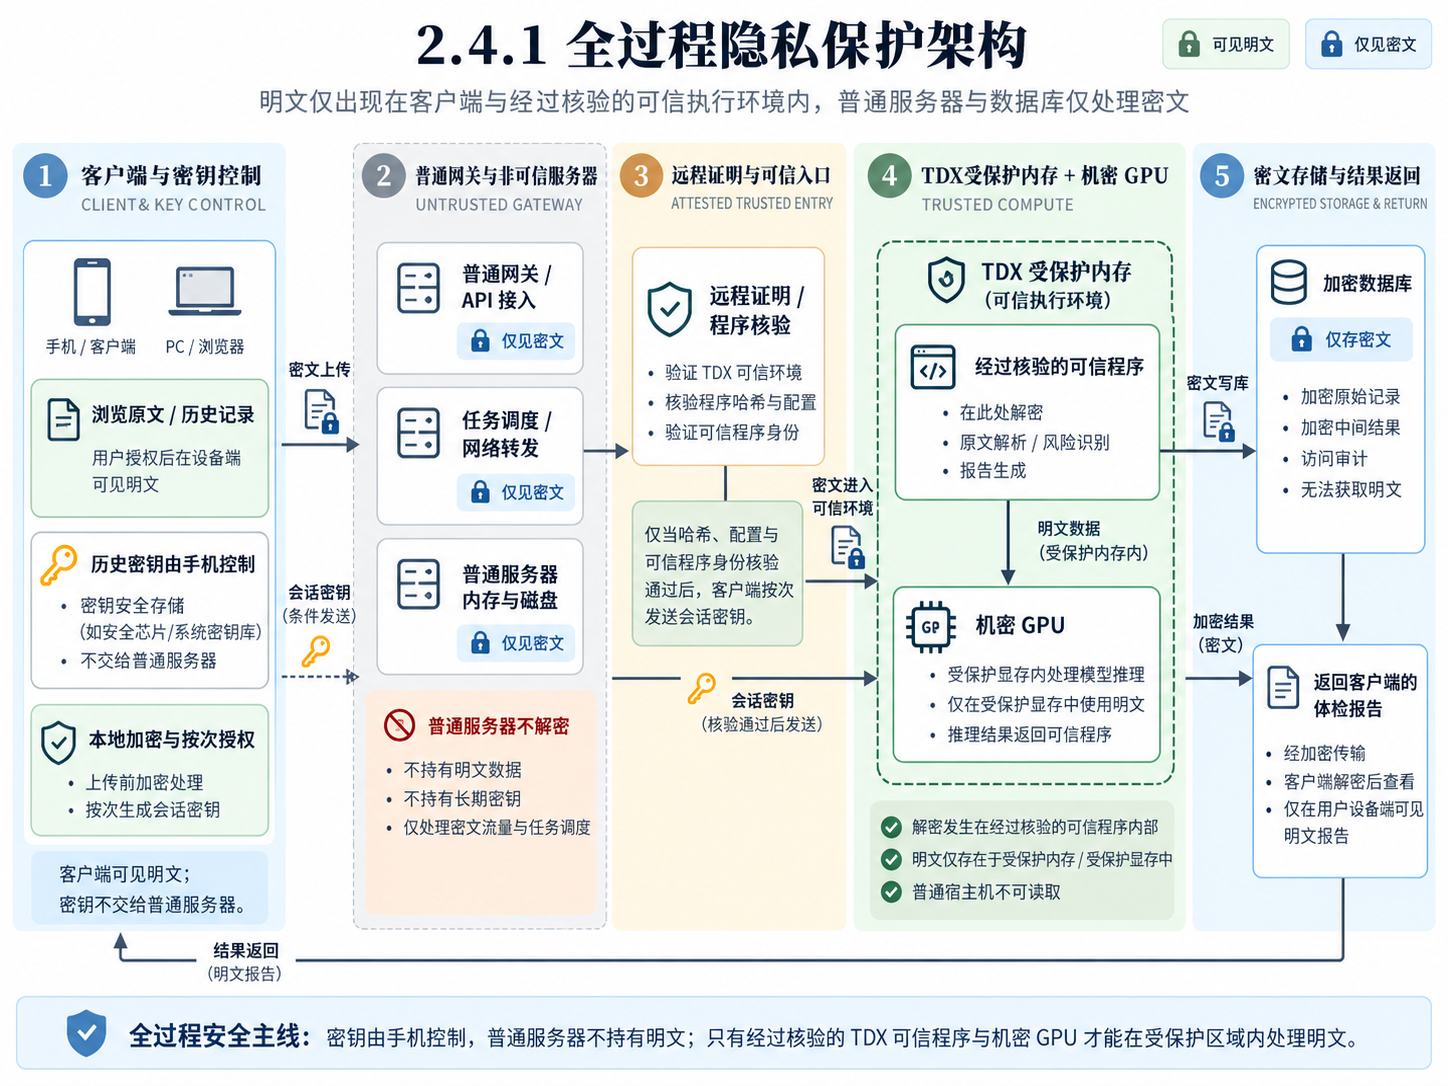
\includegraphics[width=\linewidth,height=0.72\textheight,keepaspectratio]{figures/chapter2/fig_2_5_privacy_protection.png}
\caption{全流程隐私保护架构}\label{fig:2-5}
\end{figure}

\subsubsection{防止原始内容在手机采集阶段泄露}\label{section:2.4.2}

用户的截图、音频及浏览行为首先由手机客户端采集，因此客户端本身构成隐私保护的第一道关口。即使用户已通过系统权限弹窗授权采集，也无法据此判断软件是否存在超范围记录、私自保存或向外部服务器发送数据的逻辑。一旦客户端程序存在恶意行为，后续的传输加密与云端机密计算都无法阻止原始数据泄露。因此，\textbf{手机端隐私保护的关键不仅是限制采集权限，更要保证客户端执行的是经过审查的可信程序。}

针对这一风险，破茧采用开源与安全审计相结合的程序验证机制。系统公开屏幕采集、音频处理、数据暂存及网络通信等安全关键代码，使用户及第三方能够检查数据获取范围与对外传输行为。同时，系统提供可复现构建信息，将公开源代码与实际发布的安装包建立对应关系。正式版本采用多方签名批准策略，并预留独立审核方参与审计的机制，防止未经认可的代码修改直接进入受信任的客户端版本。通过代码行为审查与发布版本验证，降低客户端利用采集权限私自获取或外传用户信息的风险。

在实际采集过程中，破茧通过Android MediaProjection获取用户授权的屏幕画面，按照端侧采样和区域裁剪规则保留必要内容，并仅在系统允许时获取音频。采集结果在应用受控内存中处理，不写入公共相册或明文日志；需要本地暂存时，采用由Android Keystore保护的密钥进行加密。由此，开源审计与版本控制约束客户端程序行为，操作系统授权限定数据获取权限，本地加密则保护必要的暂存记录。

\subsubsection{防止数据被交给未经认可的程序}\label{section:2.4.3}

上传阶段存在两条直接的泄露路径：一是通信中间节点截获数据，二是接收方被冒充。例如，服务器可以返回一把由自己掌握的公钥，让手机误以为它属于可信程序。即使云端启用了可信执行环境（TEE，即受硬件隔离的计算区域），未经审查的程序仍可能在其中解密数据并主动外传。因此，破茧需要同时验证\textbf{程序版本是否获准}与\textbf{本次加密公钥是否确实属于该程序所在的可信环境}。

与手机端的程序审核相对应，系统公开服务端的解密、模型调用、历史读写和通信等安全关键代码，固定正式版本的依赖、模型文件和安全配置，并提供可复现构建信息，使公开源码与发布产物能够对应。受认可的版本写入可信版本清单。清单采用多方签名批准策略，并预留独立审核方参与审核和签名的接口，普通业务后台不能自行增加可信版本。云端使用统一内核映像（UKI）将内核和启动配置纳入完整性测量，使用\texttt{dm-verity}校验只读系统文件，进而把允许执行的工作负载与可信启动状态对应起来。手机检查的不是服务器自行声称的代码哈希，而是硬件远程证明中记录的实际运行度量是否符合已批准清单。

在此基础上，破茧按以下步骤建立数据传输会话：

\begin{enumerate}
\def\labelenumi{\arabic{enumi}.}
\setlength{\itemsep}{0pt}\setlength{\parskip}{0pt}
\item
  \textbf{手机发出核验请求。} 客户端生成一次性随机数，要求云端提供本次运行环境的证明。可信程序在受保护的CPU内存中生成临时公私钥，私钥不交给普通网关。
\item
  \textbf{云端出具硬件证明。} Intel TDX提供可信虚拟机的启动状态和运行度量证明，NVIDIA提供GPU机密计算状态的证明。可信程序把手机随机数、临时公钥和GPU证明摘要组合成绑定值，写入TDX证明中的\texttt{REPORTDATA}字段。该字段用于证明这份材料对应的是\textbf{本次请求和本次公钥}。
\item
  \textbf{手机独立核验。} 客户端验证两类硬件证明的真实性与安全状态，核对可信虚拟机的度量值是否符合已批准版本，并检查随机数、公钥及GPU证明的绑定关系。可信程序还核对被证明的GPU就是实际承担推理的设备。任何一项不符合要求，客户端都不发送浏览内容或解密密钥。
\item
  \textbf{验证成功后加密上传。} 客户端采用HPKE（一种基于接收方公钥建立加密会话的标准机制）加密截图、音频及浏览事件。普通API网关只负责转发密文，无法凭转发权限还原数据。
\item
  \textbf{可信程序在内部解密。} 密文到达可信虚拟机后，由持有临时私钥的破茧接收程序在受保护的CPU内存中解密，再交给后续模型处理。解密不经过普通业务服务器，也不由云平台管理控制台执行。
\end{enumerate}

TDX远程证明直接反映的是虚拟机状态，并不会自动证明任意应用进程都可信。因此，系统将固定工作负载、受验证启动、程序访问权限和会话密钥绑定共同纳入准入条件，使获得解密权限的对象对应到批准的接收程序。这样，运营方即使能够转发请求、管理实例，也不能仅靠更换程序或公钥取得用户明文。

\subsubsection{防止明文在CPU与GPU计算期间泄露}\label{section:2.4.4}

数据进入可信程序后必须暂时解密，否则OCR无法读取像素，语义模型也无法理解文本。此时的风险不再是网络窃听，而是计算设备本身：普通云服务器的管理权限可能触及进程内存，模型推理还会使数据进入GPU显存。如果只保护CPU而不保护GPU，明文仍可能在显卡或两者之间的传输过程中暴露。

破茧采用阿里云\texttt{ecs.gn8v-tee.4xlarge}异构机密计算实例。Intel TDX为可信虚拟机提供CPU内存隔离，限制宿主机及虚拟化管理层对受保护数据的访问；NVIDIA GPU机密计算保护GPU中的敏感数据。可信虚拟机内的GPU驱动与显卡建立受保护的通信通道，使CPU与GPU之间传递的模型输入和中间结果在设备传输链路上保持加密状态。云平台提供上述硬件能力，破茧负责把自身的解密、OCR、语音转写和语义分析程序放入同一受保护的工作负载中。

解密后的截图和音频先在受保护的CPU内存中完成解码与时间对齐，再送入可信GPU进行OCR、语音转写和模型推理。2.2节的议题、观点和论据分析，以及2.3节的情绪引导识别，都在该计算边界内部进行；BM25检索、历史比较、指标统计和加密写回等操作由可信虚拟机内的CPU程序处理。用户原文、语义向量和提示词不交给外部在线模型接口，也不返回普通业务服务进行二次处理。

硬件隔离还需要与程序输出限制配合。正式可信工作负载不开放用于读取明文的远程登录与调试接口，关闭明文业务日志和内存转储，并限制未经批准的网络出口及运行时程序加载。这些限制作为可信版本配置的一部分接受完整性验证，避免程序把受保护环境内的内容通过正常输出通道带出。由此，\textbf{明文只为必要的OCR和模型推理在可信CPU内存与GPU显存中短暂存在，不因服务器的日常管理操作而对外暴露。}

\subsubsection{防止历史数据与报告在长期存储中泄露}\label{section:2.4.5}

单次计算结束后，破茧还需保存用户接触过的议题、观点、事实要点和情绪统计，以支持后续比较与认知体检。即使删除原始截图，BM25索引、语义向量和分析报告仍可能反推出用户关注的具体内容。如果数据库存储着可直接解密这些记录的密钥，前面建立的计算保护便会在长期存储阶段失效。

破茧将长期主密钥保留在用户手机，并通过Android Keystore进行本地保护。用户的浏览事件、议题和观点簇、事实要点、检索索引及认知体检报告，均使用用户控制的数据密钥进行AES-256-GCM认证加密，再写入普通数据库。数据库只保存密文与必要的记录标识，不保存长期主密钥。数据库管理者可以备份、迁移或删除记录，但不能仅凭数据库权限恢复其中的浏览内容。

当新内容需要与历史比较时，手机再次核验可信程序，\textbf{按次交付完成本次分析所需的数据密钥，用后销毁，长期主密钥始终留在手机}。可信程序在受保护内存中解密所需的历史索引，完成候选检索、全局或相关历史比较以及索引更新，并将更新结果重新加密写回。是否需要检索全部历史由2.2节的分析任务决定；无论读取范围如何，解密与检索均在可信环境内执行，而不是要求普通数据库直接查询明文。分析报告同样以密文存储，或经过本次受保护会话返回手机供用户查看。

AES-256-GCM能够检测密文被篡改，但单靠它无法识别数据库故意返回一个完整的旧版本。因此，系统还为历史状态维护版本号和完整性摘要，并由客户端保存最近确认的状态标识，核对后续读取与更新结果的连续性。会话结束时，可信程序清除临时密钥与可访问的明文缓存；没有新的用户授权，服务器不能自行恢复历史记录开展额外计算。

至此，破茧沿数据处理过程封闭了四类主要泄露途径：在手机端通过代码审核与版本验证约束采集行为，在上传前核验解密接收方，在CPU与GPU运行期间隔离明文，并在长期存储时把解密权保留给用户。\textbf{保护机制的核心不是要求服务器管理者始终可信，而是使其管理权限不足以直接取得用户的浏览明文和长期分析结果。}

\subsection{认知体检报告生成与主动反馈机制}\label{section:2.5}

前述信息茧房识别与情绪引导识别方法，已经能够对单条浏览内容及其历史关系作出判断，但用户最终需要了解的并非某条记录的分类结果，而是自己在一段时间内接触了哪些信息、哪些判断依据不断重复，以及是否存在值得进一步查证的内容。为此，破茧将浏览事件与议题、观点、论据和情绪引导记录关联，在已有分析结果的基础上生成分时段认知体检报告，并通过主题整理、信息盲区提示和主动提醒，将识别结果转化为用户可以理解和自主使用的信息。

\subsubsection{多维认知指标的汇总与报告生成}\label{section:2.5.1}

认知体检报告首先需要解决不同分析结果难以直接比较的问题。浏览时长描述用户的注意力投入，观点分布反映所接触的判断结构，信息增量说明新增了多少事实依据，情绪引导识别则刻画部分内容的推断与表达特征。如果将这些结果分别展示，用户仍然难以判断某个时段究竟因何形成较高的信息重复或情绪引导接触比例。因此，系统以浏览事件为共同时间索引，将2.2节和2.3节的分析结果统一组织到``时间窗口---议题---具体内容''的统计层次中。

系统分别维护浏览事件、浏览内容和事实依据三种统计口径。接触次数与有效浏览时长依据浏览事件计算，同一视频被反复观看时保留每次接触；已浏览内容数量依据内容标识去重，反映用户实际看过多少条不同材料；去重论据数量则根据2.2.3节的事实等价与联合覆盖结果计算，避免将多条视频重复引用的同一事实视为多项独立依据。每条记录通过内容标识、议题标识、观点簇及原文索引建立关联。一条内容涉及多个议题时，可以分别进入相应议题的分析，但总体浏览次数仍按原始事件计算，避免跨议题重复累加。

在时间组织上，系统形成小时、每日和长期三个层次的认知体检报告。小时报告以24小时浏览分布图展示一天内各时段的有效浏览时长及主要议题，用户进入某个时段后，可以查看该时段涉及的观点和内容构成。浏览事件按实际接触时间归属，跨越小时边界的有效浏览时长按对应时段分配。每日报告进一步汇总各议题的浏览内容数量、有效接触时长、观点分布、去重论据数量和信息增量率，并展示过度推断型情绪引导内容的接触次数及其时长占比，使浏览投入与实际获得的信息能够在同一议题下对照查看。

对于用户持续关注的议题，系统直接复用2.2.4节定义的观点集中度、有效观点数量、去重论据数量和信息增量率，形成可比较的时间序列。长期报告按连续有效窗口观察这些指标的变化，并呈现2.2.5节的信息茧房风险判定结果。例如，某议题的浏览时长连续增加，但主要观点始终集中于同一判断，信息增量率持续较低，报告便能够同时展示``投入时间增加''和``新增依据不足''两个现象及其历史变化。情绪引导统计则采用2.3.4节的内容级识别结果，以已完成判定的浏览事件为分母计算接触比例，避免将待核验内容直接计入已确认的情绪引导记录。

报告采用基于结构化记录的增量汇总方式。每次授权分析完成后，系统将新的浏览事件及其判别结果写入相应时间和议题的统计记录，无需为生成报告重复执行全文观点抽取或情绪识别。当历史议题归并、观点簇调整或论据覆盖关系得到修正时，系统依据原有事件关联重新计算受影响的统计结果。对于采集覆盖不足、有效记录过少或判断尚未完成的窗口，报告标明相应的数据范围，并保留风险判定中的证据不足状态。最终形成的统计结果按2.4节的机制加密保存，在用户授权的可信会话中更新，并返回手机供其查看。

\subsubsection{基于原文溯源的主题观点整理}\label{section:2.5.2}

时间分布与风险指标能够说明用户近期的信息接触特征，却无法代替对具体内容的回顾。尤其在短视频和社交平台中，同一问题的相关材料常常分散在不连续的浏览时段，中间穿插大量无关内容。用户即使接触过不同观点，也很难回忆它们分别来自哪些视频，又获得了什么事实支持。为此，破茧利用2.2节已经建立的议题档案、观点簇和论据关系，将分散的浏览内容整理为可追溯的主题观点卡片。

观点卡片以议题为入口，以已归并的观点簇为整理单位。系统首先按照用户选择的日期或历史范围，检索该议题下已经接触的观点记录，再依据2.2.2节确定的表达主体和支持、反驳关系，将真正支持某一观点的内容关联到对应卡片。被作者引用后加以反驳的观点，不计入作者支持该观点的内容数量。卡片使用2.2.3节维护的观点簇名称，展示观点的主要判断、支持它的已浏览内容数量，以及与其他观点存在的分歧关系，使用户能够直接比较同一问题下实际接触到的不同说法。

在每张卡片内部，系统进一步按照事实要点及其适用条件整理关联论据，并合并语义等价的重复依据。每项论据保留支持或反驳关系，同时展示它被多少条不同的已浏览内容引用，以及这些内容对应的原始来源。例如，十条就业视频都支持``招聘形势严峻''，但其中八条引用同一份裁员报道，卡片将分别呈现支持该观点的内容数量与去重后的论据，避免用户将多次传播误认为多项独立证据。对于能够由不同历史材料共同覆盖的复合论据，系统沿用已有事实要点关联，而不把重新组合的表述直接认定为新增事实。

观点及论据的展示内容均与原文索引建立对应关系。用户点击具体论据后，可以查看被引用的事实片段、相关观点语句及其上下文，并根据已保存的来源标识定位原网页位置或视频转写时间点。对于能够重新访问的原始内容，系统提供来源入口；对于暂时无法打开的来源，仍可查看授权分析过程中保存的相关文本片段及其出处信息。这样，主题总结不仅说明``用户看到了哪些观点''，还能够回答``这些观点由哪些材料支持''，使其成为可以反复核查的个人信息整理结果。

随着后续浏览增加，新的内容继续归入对应议题和观点簇，卡片中的关联内容、论据数量与来源记录同步更新。若历史比较确认议题或观点簇需要合并，系统按照2.2.3节的标识映射调整卡片关联，而不丢失原始来源。用户由此可以跨越不同日期持续回顾同一个问题，也能够根据卡片中呈现的观点分布与证据重复关系，发现已有信息尚未充分覆盖的部分。

\subsubsection{信息盲区提示与信息补全}\label{section:2.5.3}

观点整理让用户看到已经获得的材料，但当某一议题长期由少数观点主导时，用户更关心的是还需要了解什么。仅给出``观点集中度较高''的数值，并不能指出下一步应补充哪些信息。另一方面，个人浏览记录只能反映用户实际接触的内容，不能直接证明未出现的观点一定存在，或判定某种相反说法必然正确。因此，破茧将信息盲区提示建立在\textbf{已有浏览材料的覆盖范围}之上，重点指出当前认识所依赖的观点、事实条件及来源可能存在哪些局限。

系统首先利用2.2节形成的议题历史，比较近期窗口与较长历史范围内的观点簇和论据记录。如果某种观点曾在历史中出现、近期却很少接触，系统可以提示用户回顾该观点及原有依据；如果近期大量内容表达相似判断，而去重论据数量有限、信息增量率持续较低，则提示用户当前接触的材料主要重复了哪些事实。系统还利用事实要点中的主体、时间和地域等限定条件，归纳浏览材料实际覆盖的范围。例如，用户近期关于就业的内容主要涉及互联网企业裁员，提示便指出当前材料集中于该行业和相关事件，而不据此推断整个就业市场均呈现相同情况。

这些提示优先利用已经保存的历史记录完成。对于历史中存在的不同观点或尚未在近期出现的事实依据，系统直接关联对应的观点卡片与原文来源，帮助用户重新查看已有信息；对于历史中尚未出现的观点或事实，系统只说明``当前已浏览材料尚未覆盖''，并给出可进一步查证的方向。信息盲区由此表现为个人接触记录中的覆盖不足，而不是系统凭空生成的相反立场。

当个人历史无法提供足够的补充材料时，用户可以自主发起外部资料检索。系统根据当前议题名称及需要补充的事实维度，形成不包含个人浏览原文和行为记录的通用检索词，由用户确认后通过手机端发起查询。对于就业议题，补充方向可以是其他行业的招聘数据、不同地区的就业统计，或相关调查报告的原始出处。检索结果按照发布时间、来源及事实适用条件展示，重点寻找能够增加独立依据或扩展观察范围的材料，而不是机械推荐与现有观点相反的内容。

用户选择进一步分析外部资料时，候选文本可以经重新核验的加密会话进入可信计算环境，复用2.2节的议题匹配与论据比较方法，检查它相对于个人历史是否提供了新的事实要点。外部检索结果在用户实际阅读前，仅作为待查看的补充资料，不计入已浏览内容数量及信息增量率。该功能采用用户按需发起的方式，不依赖持续的外部网络检索；客户端同时向用户说明，外部检索服务可能获知其主动提交的查询词，用户可以修改关键词或完全不使用此功能。通过区分已有历史回顾与外部资料补充，系统既能够指出信息覆盖不足，也将是否扩展信息来源的决定权交给用户。

\subsubsection{风险提醒与用户自主交互}\label{section:2.5.4}

认知体检报告主要支持用户主动回顾，但观点长期集中或过度推断型情绪引导反复出现时，用户未必会及时打开报告。为使长期分析结果能够在需要时发挥作用，破茧将已经完成核验的风险记录转换为可查看依据的提醒，并通过用户设置控制提醒时机与频率。提醒的目标是提示当前浏览材料值得复核，而不是替代用户判断内容是否真实，或推断用户已经产生了某种情绪变化。

信息茧房提醒直接以2.2.5节的长期风险判定为依据。当某个议题在足够数量的有效窗口中持续满足观点集中与信息增量不足的联合条件，且风险状态为触发预警时，系统生成对应提示；处于证据不足状态的议题不触发该类预警。情绪引导提醒则使用2.3节已经完成原文核验的内容级结果：当预设时间窗口内此类内容达到最低接触次数，且其数量占比或有效浏览时长占比达到提醒阈值时，系统才生成相应提示。两类提醒分别依据长期信息重复模式和已确认的过度推断型情绪引导接触情况，不将单次浏览或普通负面信息直接视为风险。

提醒内容由可信计算环境依据风险类型及关联原文记录形成，通过受保护会话交付手机客户端，由手机本地展示通知。通知首页仅使用简要、非敏感的提示文字，具体议题、观点和浏览内容在用户打开应用后展示，避免通过普通推送服务暴露个人关注的问题。由于2.4节的历史解密机制依赖用户按次授权，系统只针对已获授权并完成分析的记录更新提醒；没有有效授权会话时，云端不自行解密历史数据进行后台扫描，后续提醒在客户端下一次获得相应分析结果时合并呈现。

为减少持续信息流中的重复打扰，系统按照议题和提醒类型维护通知状态。同一议题的相同风险在设定的间隔内只提示一次；若风险条件仍然持续，但没有出现新的实质性依据，则合并进入每日报告，不反复推送。多个相关记录在短时间内触发时，系统优先合并为一条汇总提醒。用户可以选择仅接收每日摘要、设置免打扰时段、调整提醒频率，也可以关闭特定议题或某类风险的通知，使认知安全提示服从实际使用需要。

用户打开提醒后，系统提供从结论返回依据的查看路径。对于信息茧房提醒，页面展示对应时间窗口的主导观点比例、信息增量变化，以及反复出现的事实要点与来源；对于情绪引导提醒，页面展示原文中被引用的事实、相关结论及识别出的范围外推或确定程度提高，并标明负面强化方式。用户可以进入相应观点卡片查看完整上下文，也可以对议题归属、观点归并或原文对应关系提出纠正。涉及分析记录的修正由后续授权的可信程序重新核验，并更新受影响的统计结果与提醒状态。

通过以上机制，破茧将连续浏览产生的内容分析结果组织为可回顾、可追溯的认知体检报告，再由报告中的观点与论据关系发现信息覆盖局限，并在长期风险成立时提供适度提醒。用户能够据此回顾实际获得的判断依据，自主选择是否查阅补充资料，以及如何接收和使用提示，使个人认知安全防护与日常信息管理形成连续的使用过程。

% 第三章正文，直接编辑本文件。
\FloatBarrier\clearpage

\section{作品测试与分析}\label{chapter:3}

本章对破茧系统的功能、分析效果、运行性能与安全性进行测试，重点评价浏览记录、观点与论据识别、个人历史比较及长期接触模式分析的准确性，并验证可信执行环境中的数据保护机制。测试既检查浏览作品能否被正确记录，也检查观点与论据能否回到已观察证据、历史比较是否遵循事件时间、持续接触模式是否得到合理解释，以及个人数据是否在授权的可信边界内处理。评价对象为系统在明确观察范围内的工程行为与分析能力，不将内容接触解释为用户认同，不以单一主题集中或内容焦虑表达代替信息茧房及个人心理状态判断。

\subsection{测试目标与总体方案}\label{section:3.1}

\subsubsection{测试目标}\label{section:3.1.1}

测试覆盖内容采集、语义分析、历史检索、状态维护和报告展示等环节。采集层验证作品身份、观看事件和观察片段的区分，避免将采样次数当作作品数量；语义层验证对象条件化的跨模态对齐、主体归属、论证结构和证据定位；历史层验证双路检索、联合覆盖和五维增量；时序层验证低增量重复的持续性及与正常专题学习的区分；安全层验证证明绑定、密钥释放、加密消息与历史检查点；报告层验证统计守恒、未知状态、证据追溯与用户更正。

验收采用功能约束和统计指标相结合的方法。用户隔离、事件幂等、历史时间边界和无效证明拒绝属于必须满足的工程约束；作品识别、论证抽取和接触模式识别使用精确率、召回率、F1 及校准误差评价。各项指标仅对其有效输入范围作出结论，未观察区域及不具备分析依据的样本分别列示。

\subsubsection{测试范围与方法}\label{section:3.1.2}

\begin{longtable}[]{@{}
  >{\RaggedRight\arraybackslash}p{(\linewidth - 8\tabcolsep) * \real{0.1600}}
  >{\RaggedRight\arraybackslash}p{(\linewidth - 8\tabcolsep) * \real{0.2500}}
  >{\RaggedRight\arraybackslash}p{(\linewidth - 8\tabcolsep) * \real{0.2500}}
  >{\RaggedRight\arraybackslash}p{(\linewidth - 8\tabcolsep) * \real{0.2500}}
  >{\RaggedRight\arraybackslash}p{(\linewidth - 8\tabcolsep) * \real{0.0900}}@{}}
\caption{测试范围、目标与评价指标}\label{tab:3-1}\tabularnewline
\toprule\noalign{}
测试模块 & 测试对象及主要输入 & 预期行为 & 主要评价指标 & 结果状态 \\
\midrule\noalign{}
\endfirsthead
\toprule\noalign{}
测试模块 & 测试对象及主要输入 & 预期行为 & 主要评价指标 & 结果状态 \\
\midrule\noalign{}
\endhead
\bottomrule\noalign{}
\endlastfoot
内容对象、事件、语义结果 & 同作品多次打开及同事件多版本 & 三类标识独立，修订不新增观看事件 & 身份一致性、修订一致性 & 通过 \\
增量采集 & 页面变化、图文翻页、关键帧、字幕及音频片段 & 只处理授权可见片段，标记缺口 & 作品计数 P/R、采样去重、覆盖率 & 达标 \\
阅读投入估计 & 正文与评论共屏、滚动、触控、未定位区间 & 时间分配守恒，弱线索不等于实际阅读 & 可见区间 MAE、分配误差、未定位率 & 达标 \\
联合论证理解 & 文字、图像与音频观察版本 & 正确归属主体、条件和论据，输出可定位证据 & 字段 macro-F1、主体准确率、证据定位 & 达标 \\
个人历史增量 & 当前论证及严格过去的多条历史 & 区分复述与新增事实、论据、条件、解释、行动 & Recall@50、五维 macro-F1、联合覆盖 F1 & 达标 \\
时序论证图 & 多日事件、异构关系、缺失掩码及阅读权重 & 识别接触模式，避免专题学习误报 & macro-F1、误报率、ECE & 达标 \\
机密计算 & 证明、报文、加密对象、检查点与删除事务 & 未经放行不释放密钥，拒绝篡改和旧状态 & 拒绝率、状态一致性、恢复开销 & 通过 \\
情绪联合建模 & 情绪---原因候选对、角色及自愿反馈 & 分开呈现内容表达与个人反馈 & 配对 F1、角色 F1、有序误差 & 达标 \\
异步分析 & 突发输入、迟到事件、超时、重连 & 阶段结果可用、队列稳定、最终一致 & 接收 P95、完成 P95、积压及恢复时间 & 达标 \\
聚合展示 & 小时、自然日、滚动窗口及多设备重叠 & 分母明确、时间守恒、证据可回看 & 聚合一致性、追溯完整性 & 通过 \\
\end{longtable}

单元测试验证字段、区间和密码接口；服务测试验证事件状态与授权；端到端测试对照人工操作轨迹；离线模型评价使用隔离测试集；性能测试按固定负载回放；安全测试按协议状态注入异常。训练超参数、判定阈值和置信校准仅使用训练与验证数据，测试集在模型与配置冻结后一次性评价。模型实验使用 3 个随机种子，表中报告均值；置信区间按原始作品或用户整组重采样，而不是按同作品的观察版本独立重采样。

\subsection{测试环境搭建与设备}\label{section:3.2}

\subsubsection{端侧与浏览器环境}\label{section:3.2.1}

手机测试覆盖 OPPO/ColorOS、vivo/OriginOS、小米/HyperOS、荣耀/MagicOS、三星/One UI 及 Pixel/原生 Android 六类终端，每类设置 2 台设备，共 12 台物理设备。测试涵盖 Android 12 至 14、8 至 12 GB 内存及 60 Hz 和 120 Hz 显示模式，重点检查无障碍节点差异、后台运行限制、屏幕采集授权和作品切换时的状态保持。受控测试应用提供可核验的作品标识、固定操作脚本和显示时间；真实平台测试采用授权操作轨迹，平台版本随测试批次固定。Android 模拟器用于异常流程复现，不替代真机前台流畅度与页面识别评价。

浏览器端使用 Chromium 环境，通过具有明确内容标识的受控网页核对 DOM 增量、正文与评论分离、鼠标悬停线索和窗口可见性。手机和浏览器均使用单调时钟测量持续时长，设备时钟用于事件时间与时区归档，服务器接收时间独立记录。网络条件包括稳定 Wi-Fi、蜂窝网络和受控弱网；弱网注入 100 毫秒附加往返时延、1\%丢包及 60 秒断网，分开评价网络开销与服务计算开销。

\subsubsection{云端计算与可信环境}\label{section:3.2.2}

\begin{longtable}[]{@{}
  >{\RaggedRight\arraybackslash}p{(\linewidth - 6\tabcolsep) * \real{0.1600}}
  >{\RaggedRight\arraybackslash}p{(\linewidth - 6\tabcolsep) * \real{0.2800}}
  >{\RaggedRight\arraybackslash}p{(\linewidth - 6\tabcolsep) * \real{0.2800}}
  >{\RaggedRight\arraybackslash}p{(\linewidth - 6\tabcolsep) * \real{0.2800}}@{}}
\caption{云端测试设备与用途}\label{tab:3-2}\tabularnewline
\toprule\noalign{}
环境 & 公开云实例及配置 & 使用范围 & 可信边界 \\
\midrule\noalign{}
\endfirsthead
\toprule\noalign{}
环境 & 公开云实例及配置 & 使用范围 & 可信边界 \\
\midrule\noalign{}
\endhead
\bottomrule\noalign{}
\endlastfoot
普通 GPU 环境 & AWS EC2 g5.2xlarge；8 vCPU、32 GiB 内存、1 张 NVIDIA A10G，产品页标称 24 GB GPU 内存 & 脱敏数据基线、负载发生与轻量组件对照 & 不作为本项目机密 GPU 证明环境 \\
CPU 机密环境 & Azure Standard\_\allowbreak{}DC8as\_\allowbreak{}v5；8 vCPU、32 GiB 内存、AMD SEV-SNP，无 GPU & CPU 可信处理、检索、状态事务及协议验证 & 客体操作系统与获准服务属于可信计算基 \\
GPU 机密环境 & Azure Standard\_\allowbreak{}NCC40ads\_\allowbreak{}H100\_\allowbreak{}v5；40 vCPU、320 GiB 内存、1 张 H100 NVL，94 GB GPU 内存 & 多模态联合模型、异步推理、真实机密 GPU 测试 & 经验证的 CPU、GPU 及其受保护通信链路 \\
\end{longtable}

测试采用表~\ref{tab:3-2}所列云端环境，普通 GPU 用于基线对照，CPU 机密环境用于受保护检索与状态事务，机密 GPU 环境用于多模态推理及性能评价。

\begin{longtable}[]{@{}
  >{\RaggedRight\arraybackslash}p{(\linewidth - 4\tabcolsep) * \real{0.2000}}
  >{\RaggedRight\arraybackslash}p{(\linewidth - 4\tabcolsep) * \real{0.4000}}
  >{\RaggedRight\arraybackslash}p{(\linewidth - 4\tabcolsep) * \real{0.4000}}@{}}
\caption{软件测试配置}\label{tab:3-3}\tabularnewline
\toprule\noalign{}
组件 & 实验配置 & 用途与约束 \\
\midrule\noalign{}
\endfirsthead
\toprule\noalign{}
组件 & 实验配置 & 用途与约束 \\
\midrule\noalign{}
\endhead
\bottomrule\noalign{}
\endlastfoot
客体系统 & Ubuntu 22.04 LTS，机密实例使用厂商兼容镜像 & 常规/机密对照分别记录镜像摘要 \\
Python 与训练 & Python 3.11、PyTorch 2.5、CUDA 12.4 兼容运行时 & LoRA、任务头训练和推理 \\
OCR 与 ASR & PaddleOCR 2.9、Whisper large-v3-turbo & 固定识别器权重与预处理配置 \\
移动客户端 & Kotlin、Android SDK 34、Compose、Room & 事件、区间与版本管理 \\
密码与证明 & OpenSSL 3.0 系列、厂商证明 SDK & 固定安全补丁与验证材料，不自行实现密码原语 \\
浏览器 & Chromium 128 兼容测试环境 & 受控 DOM、可见性与交互轨迹 \\
\end{longtable}

各组实验采用一致的软件版本、模型权重与预处理配置。服务采用 Linux 客体系统，固定组件和模型版本。镜像、模型权重、提示模板、工具权限和分析配置组成版本清单，加载器验证摘要后锁定会话版本。日志只保留不透明任务编号、阶段状态及资源指标，原文、向量和诊断详情保存在用户授权的受保护对象内。

协议联调使用明确标识的 Mock 证明；CPU 与 GPU 机密执行使用硬件证明和相应验证链。GPU 配置核验参考 Azure 机密 GPU 说明\cite{ref33}。只有 CPU 隔离不能证明 GPU 张量及设备内存受到相同保护，普通 GPU 结果不计入机密 GPU 安全结论。

\subsubsection{实验控制与测量方法}\label{section:3.2.3}

模型评价固定输入版本和观察范围。精细理解采用不超过 2,048 个文本 token、最多 8 张关键帧及 30 秒已授权音频片段的单任务上限，长视频按片段处理并保留关联。训练在 GPU 环境中使用 LoRA 及任务头联合学习，公共语料仅承担其已具备字段的迁移监督，中文目标域负责本项目字段与置信校准。任务掩码跳过缺失标签，不将未标注字段作为负例。

性能测试固定 50\%纯文字、30\%图文和 20\%视频片段的事件混合比例，每事件平均触发 1 次初步理解、0.5 次 OCR、0.2 次 ASR、0.3 次跨模态精细理解、1 次历史比较及 1 次图更新。批处理上限为 8，模型和版本策略固定，比较机密与常规执行时使用相同硬件规格及输入序列。A10G 与 H100 跨硬件差异不用于推导机密计算开销。

\subsection{测试数据与标注规范}\label{section:3.3}

\subsubsection{数据集构成}\label{section:3.3.1}

\begin{longtable}[]{@{}
  >{\RaggedRight\arraybackslash}p{(\linewidth - 6\tabcolsep) * \real{0.2500}}
  >{\RaggedRight\arraybackslash}p{(\linewidth - 6\tabcolsep) * \real{0.2500}}
  >{\RaggedRight\arraybackslash}p{(\linewidth - 6\tabcolsep) * \real{0.2500}}
  >{\RaggedRight\arraybackslash}p{(\linewidth - 6\tabcolsep) * \real{0.2500}}@{}}
\caption{自建数据集及评价用途}\label{tab:3-4}\tabularnewline
\toprule\noalign{}
数据集 & 规模与组成 & 核心标注 & 评价用途 \\
\midrule\noalign{}
\endfirsthead
\toprule\noalign{}
数据集 & 规模与组成 & 核心标注 & 评价用途 \\
\midrule\noalign{}
\endhead
\bottomrule\noalign{}
\endlastfoot
跨平台多模态作品与论证 & 6,000 个作品；小红书图文、小红书短视频、抖音短视频各 2,000 个；每作品 3 个观察版本，共 18,000 个版本 & 对象、主体、观点短语、立场、条件、论据、引用/反驳及证据索引 & 多模态理解与部分观察修订 \\
个人历史信息增量 & 12,000 组当前材料---过去历史样本，每组允许多条历史 & 五维增量、联合覆盖、同源关系、证据不足 & 检索、关系判断与信息增量 \\
长期接触序列 & 200 名自愿参与者，每人 14 天，共 2,800 个用户日 & 有效观察、接触模式、阅读目的、回顾依据 & 时序图、校准及长期解释 \\
情绪---原因---角色 & 8,000 个上下文片段，来自上述作品 & 情绪与原因跨度、持有者、对象、归属、认知评价、处境、表达方式 & 联合情绪模型及反馈分离 \\
页面与安全回归 & 240 条操作轨迹，两平台各 120 条；120 个协议与状态场景 & 真实作品边界、可见区间、状态转移及拒绝条件 & 计数、停留估计及安全一致性 \\
\end{longtable}

作品采样覆盖就业与教育、性别与家庭、科技与产品、经济与消费、健康与生活、公共议题六类领域，每类 1,000 个作品。领域用于采样分层，实际观点使用``当前招聘困难''\,``职业能力需要持续提升''等可回到原文的短语，并保留对象、时态和条件，不将``经济与消费''等领域名称作为观点结论。

数据记录包括平台内标识、匿名作者标识、时间、可见正文、授权媒体、OCR/ASR 片段、评论线程及覆盖范围。授权按参与者、应用和媒体类型分别管理，授权撤回与删除操作均进入测试流程；私人聊天、未授权后台内容与隐藏页面不进入语料。数据获取不绕过平台权限和访问限制，身份映射与分析材料分开保存。模型训练使用经过单独授权和脱敏处理的材料，不将参与者全部个人历史默认用于训练。

样本来源、授权范围和撤回状态分别记录，数据使用限定在参与者同意的研究范围内。

\subsubsection{数据划分与泄漏防范}\label{section:3.3.2}

原始作品按作者、作品身份及同源近重复组统一划分，训练/验证/测试分别为 4,200/900/900 个作品，相应观察版本为 12,600/2,700/2,700 个。依赖作品的增量样本和情绪样本继承同一划分：增量样本为 8,400/1,800/1,800 组，情绪片段为 5,600/1,200/1,200 条。分层组分配在构建样本之前完成，跨组依赖样本不纳入本轮划分；同一作品的早期与完整版本不会分别进入训练和测试。

测试集作品在六个领域各 150 个，三种平台/媒体组合各 300 个。增量测试集覆盖八类情形，每类 225 组，共 1,800 组：同观点新论据、同义改写重复、条件扩展、解释变化、行动变化、引用后反驳、同源转载和证据不足。这些情形用于分层抽样而非互斥的五维增量标签，一个样本可以同时包含多种增量。

长期评价设置两套独立协议。用户隔离协议采用 140/30/30 名用户，分别对应 1,960/420/420 个用户日；测试用户的个性化反馈不能用于训练。时间隔离协议在全部 200 名用户内按前 8 天、随后 3 天、最后 3 天划分，分别为 1,600/600/600 个用户日，只有早期反馈参与个体适配。两套协议的结果分别报告，不相加为独立样本总量。测试期历史可作为当时已观察上下文，但其测试标签不参与参数更新或调阈值。

用户日表示安排的观察单位，不代表全天完整采集。缺失区间按原因和持续时间保存，没有观测的日期标为缺失。历史比较对每次当前观察采用严格小于该观察时点的材料，并读取当时已可用版本；后续补充、未来评论及后来取得的完整视频不进入早期历史判断。

\subsubsection{标注与一致性}\label{section:3.3.3}

语义样本由两名标注者独立标注，第三人裁决分歧。观点、立场和条件标签一致性使用 Cohen's κ，论证与情绪跨度使用标注者间 F1，有序评价使用加权κ。实验中立场κ为 0.84，增量标签平均κ为 0.79，论证证据跨度 F1 为 0.88，情绪---原因配对 F1 为 0.85，有序认知评价加权κ为 0.76。裁决后保留争议类型及支持片段，而不将一致性数值解释为标注完全正确。

认知评价采用目标受阻、威胁或损失、结果不确定性、自身控制可能、应对资源五个维度。每维使用五级强度，缺乏材料或未提及单独记录适用性。内容人物的表达、引述人物的表达与参与者自报分别标注，不能用页面停留时间自动生成个人情绪标签。

\subsection{功能、采集与统计一致性测试}\label{section:3.4}

\subsubsection{作品计数及可见停留}\label{section:3.4.1}

240 条轨迹共包含 2,920 次进入作品的观看事件。对每条轨迹按平台和人工核验作品标识去重后，累计为 2,540 个轨迹内作品；同作品再次打开增加观看事件，不增加该轨迹内去重作品数。单次观看中的文案展开、图像翻页和评论开关增加片段或修订，不增加作品数。

计数识别输出 2,900 次候选事件，与人工边界匹配得到 TP=2,856、FP=44、FN=64，精确率为 98.48\%，召回率为 97.81\%，F1 为 98.14\%，达到两项均不低于 95\%的验收要求。匹配使用作品身份和时间重叠联合约束，每个预测与真值至多匹配一次。错误集中在极快切换、遮挡过渡与平台页面结构变化，说明系统减少了重复计数，但未达到任意页面下完全不重不漏。

按区间端点计算的可见停留 MAE 为 1.12 秒，P95 绝对误差为 2.80 秒；验收约束作用于 MAE 而非所有样本最大误差。正文与评论阅读投入以人工回顾定位作为参考，平均时长绝对误差为 1.65 秒，未定位时长占有效观察时长的 8.6\%。该项衡量估计与参考的一致性，不等同于眼动测量或认知投入真值。

\subsubsection{状态、恢复与报告验证}\label{section:3.4.2}

\begin{longtable}[]{@{}
  >{\RaggedRight\arraybackslash}p{(\linewidth - 10\tabcolsep) * \real{0.0800}}
  >{\RaggedRight\arraybackslash}p{(\linewidth - 10\tabcolsep) * \real{0.1300}}
  >{\RaggedRight\arraybackslash}p{(\linewidth - 10\tabcolsep) * \real{0.2200}}
  >{\RaggedRight\arraybackslash}p{(\linewidth - 10\tabcolsep) * \real{0.2300}}
  >{\RaggedRight\arraybackslash}p{(\linewidth - 10\tabcolsep) * \real{0.2600}}
  >{\RaggedRight\arraybackslash}p{(\linewidth - 10\tabcolsep) * \real{0.0800}}@{}}
\caption{功能及一致性用例}\label{tab:3-5}\tabularnewline
\toprule\noalign{}
用例编号 & 测试对象 & 输入或步骤 & 预期结果 & 评价指标与结果 & 状态 \\
\midrule\noalign{}
\endfirsthead
\toprule\noalign{}
用例编号 & 测试对象 & 输入或步骤 & 预期结果 & 评价指标与结果 & 状态 \\
\midrule\noalign{}
\endhead
\bottomrule\noalign{}
\endlastfoot
TC-01 & 同作品增量 & 翻页、字幕新增、文案展开及评论开关 & 原事件修订，作品身份稳定 & 与人工计数联合核验，P=98.48\%、R=97.81\% & 达标 \\
TC-02 & 事件幂等 & 相同事件与修订重复发送，重复与并发混合 & 返回已有状态，统计贡献一次 & 10,000 次提交的贡献一致性 100\% & 通过 \\
TC-03 & 修订替换 & 修改观点或补充媒体片段 & 先撤销旧贡献再应用新贡献 & 1,000 组序列无重复贡献 & 通过 \\
TC-04 & 迟到及时间边界 & 断网补传、乱序、未来版本与同时间事件 & 严格过去历史，重算受影响范围 & 600 组时间用例全部符合预期 & 通过 \\
TC-05 & 中断恢复 & 阶段任务重启与 60 秒断网 & 重试不新增事件，阶段可恢复 & 300 次恢复后版本及摘要一致 & 通过 \\
TC-06 & 多用户隔离 & 相同标识、不同凭据，跨用户检索和删除 & 拒绝越权，缓存和记忆隔离 & 500 组隔离请求无跨用户对象返回 & 通过 \\
TC-07 & 多设备重叠 & 两设备同时间浏览与跨小时事件 & 单设备分别展示，个人时间取并集 & 500 组区间用例守恒 & 通过 \\
TC-08 & 时区聚合 & 自然日、滚动 24 小时、7 天及夏令时切换 & 真实时长按时区偏移分桶 & 240 组窗口用例分子分母一致 & 通过 \\
TC-09 & 证据回看 & 点击小时、观点及历史关系 & 返回对应修订与原文/媒体位置 & 900 个测试作品的索引结构完整 & 通过 \\
TC-10 & 用户更正及删除 & 修改归属、删除原事件及派生依赖 & 新报告不引用已删除对象 & 300 组依赖重算与报告检查通过 & 通过 \\
\end{longtable}

上述功能用例与 240 条轨迹及 120 个安全场景是不同计数单位：功能用例由场景参数化生成，不另充当自然作品或独立模型样本。工程约束用例全部通过只说明约定输入满足规则，不代表语义模型准确率为 100\%。

日报按自然日展示，过去 24 小时按查询截止点回溯，最近 7 天同时标明观察有效日数。未知观点、证据不足、等待处理与采集失败分别统计。观点采用多标签，比例以同一窗口内可分析去重作品为分母，允许合计超过 100\%；未知作品另列，不把多标签比例画成互斥饼图。需要饼图时仅展示主观点分配，并显式保留混合及未定位类别。

\subsubsection{同一作品多片段的端到端验证}\label{section:3.4.3}

本项测试验证页面变化是否被错误当成作品切换。小红书图文作品 W-A 的观看事件 E-A 于 10:59:42 开始、11:00:18 结束，共 36 秒。操作依次为阅读正文 12 秒、翻阅图片 8 秒、打开评论 10 秒、返回正文 6 秒。系统生成 4 次内容修订，保持作品数 1、观看次数 1，正文与图片分配 26 秒、评论 10 秒，合计不超过可见区间。案例内容依据本章数据集设定构造，不冒充真实个人记录或平台截图。

作品讨论``就业需要结合行业差异''。正文写有``不同岗位不能一概而论''，第二张图提供行业分组，评论中出现被反驳的``所有行业都没有机会''。理解模块保留作者观点、图片论据及评论引用/反驳关系，不把评论表达归给正文作者。图片翻页使论据由未定位修订为已定位，不产生新作品。

小时聚合分别计入 10 时段 18 秒和 11 时段 18 秒，两小时各包含 1 个作品，但日去重作品仍为 1。小时作品数不能简单相加为日作品数；跨小时的同一事件在详情中明确标识。点击任一小时能够回看同一事件及对应片段，修订替换旧贡献而不重复累加。

\begin{figure}[htbp]
\centering
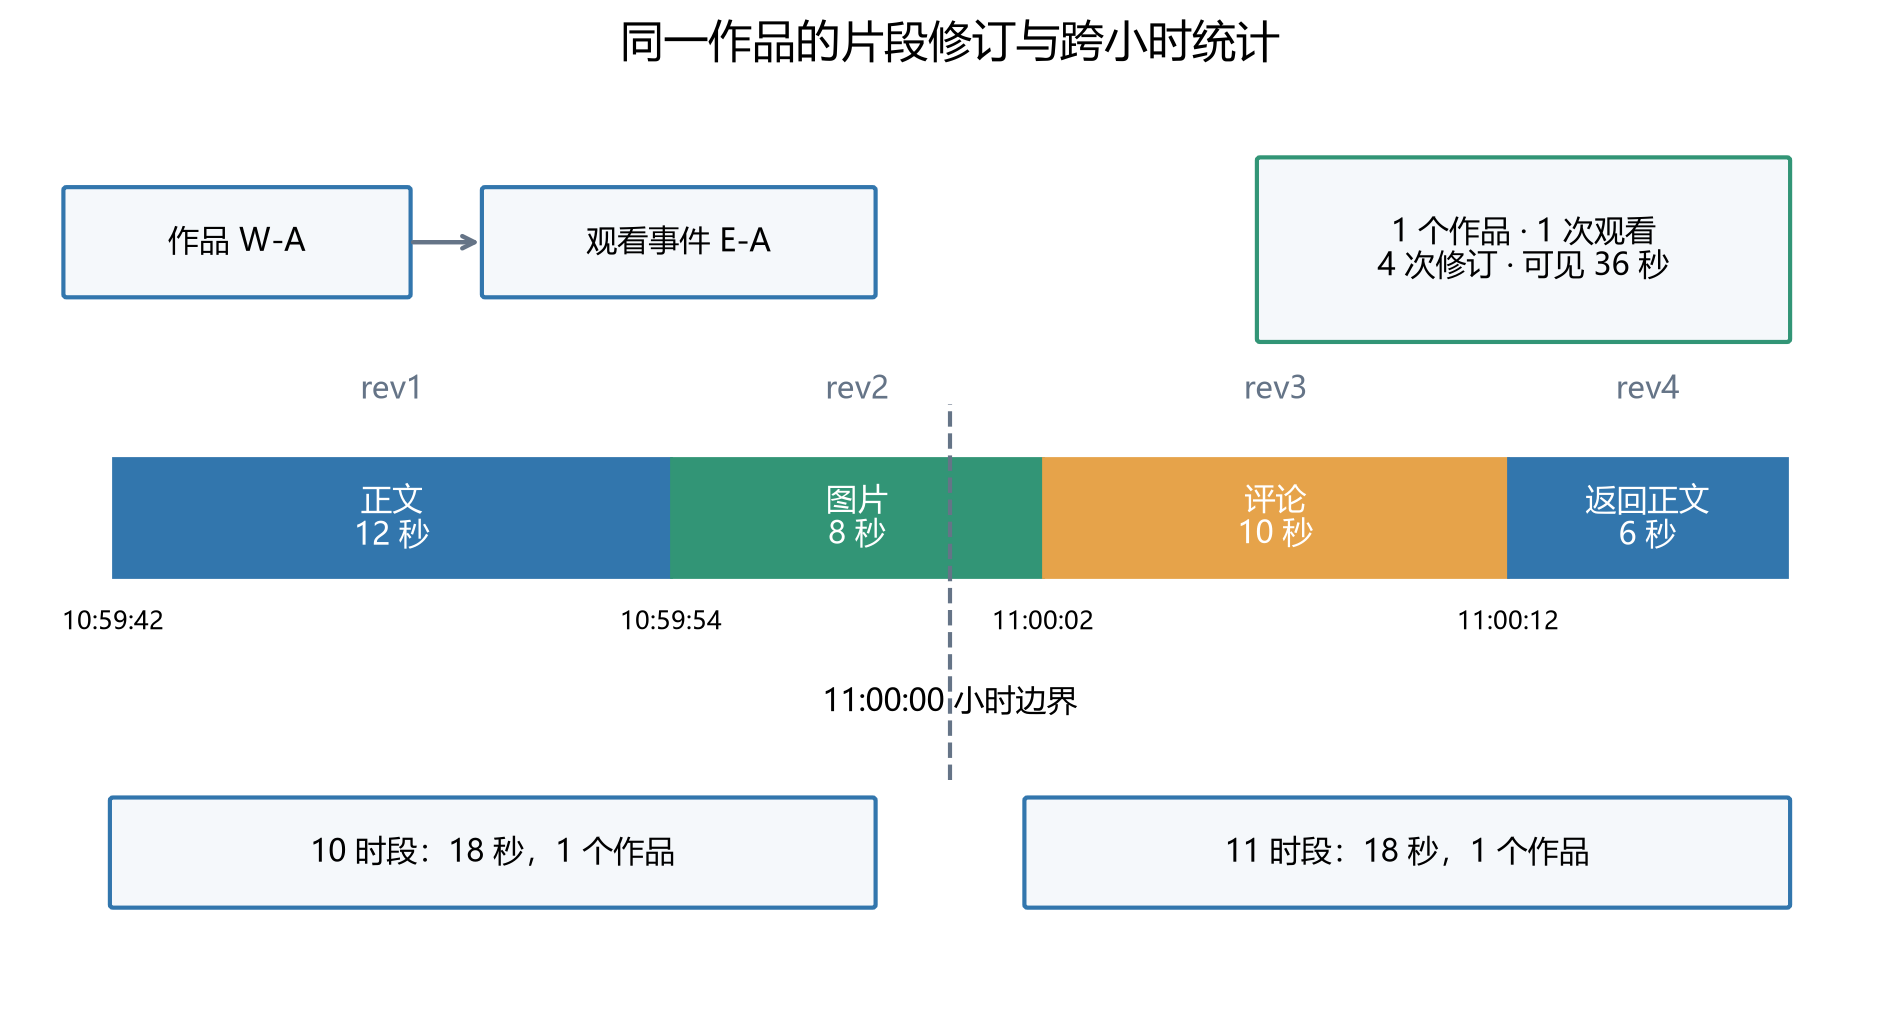
\includegraphics[width=\linewidth,height=0.66\textheight,keepaspectratio]{figures/chapter3/图3-1.png}
\caption{同一作品的片段修订与跨小时统计}\label{fig:3-1}
\end{figure}

\begin{figure}[htbp]
\centering
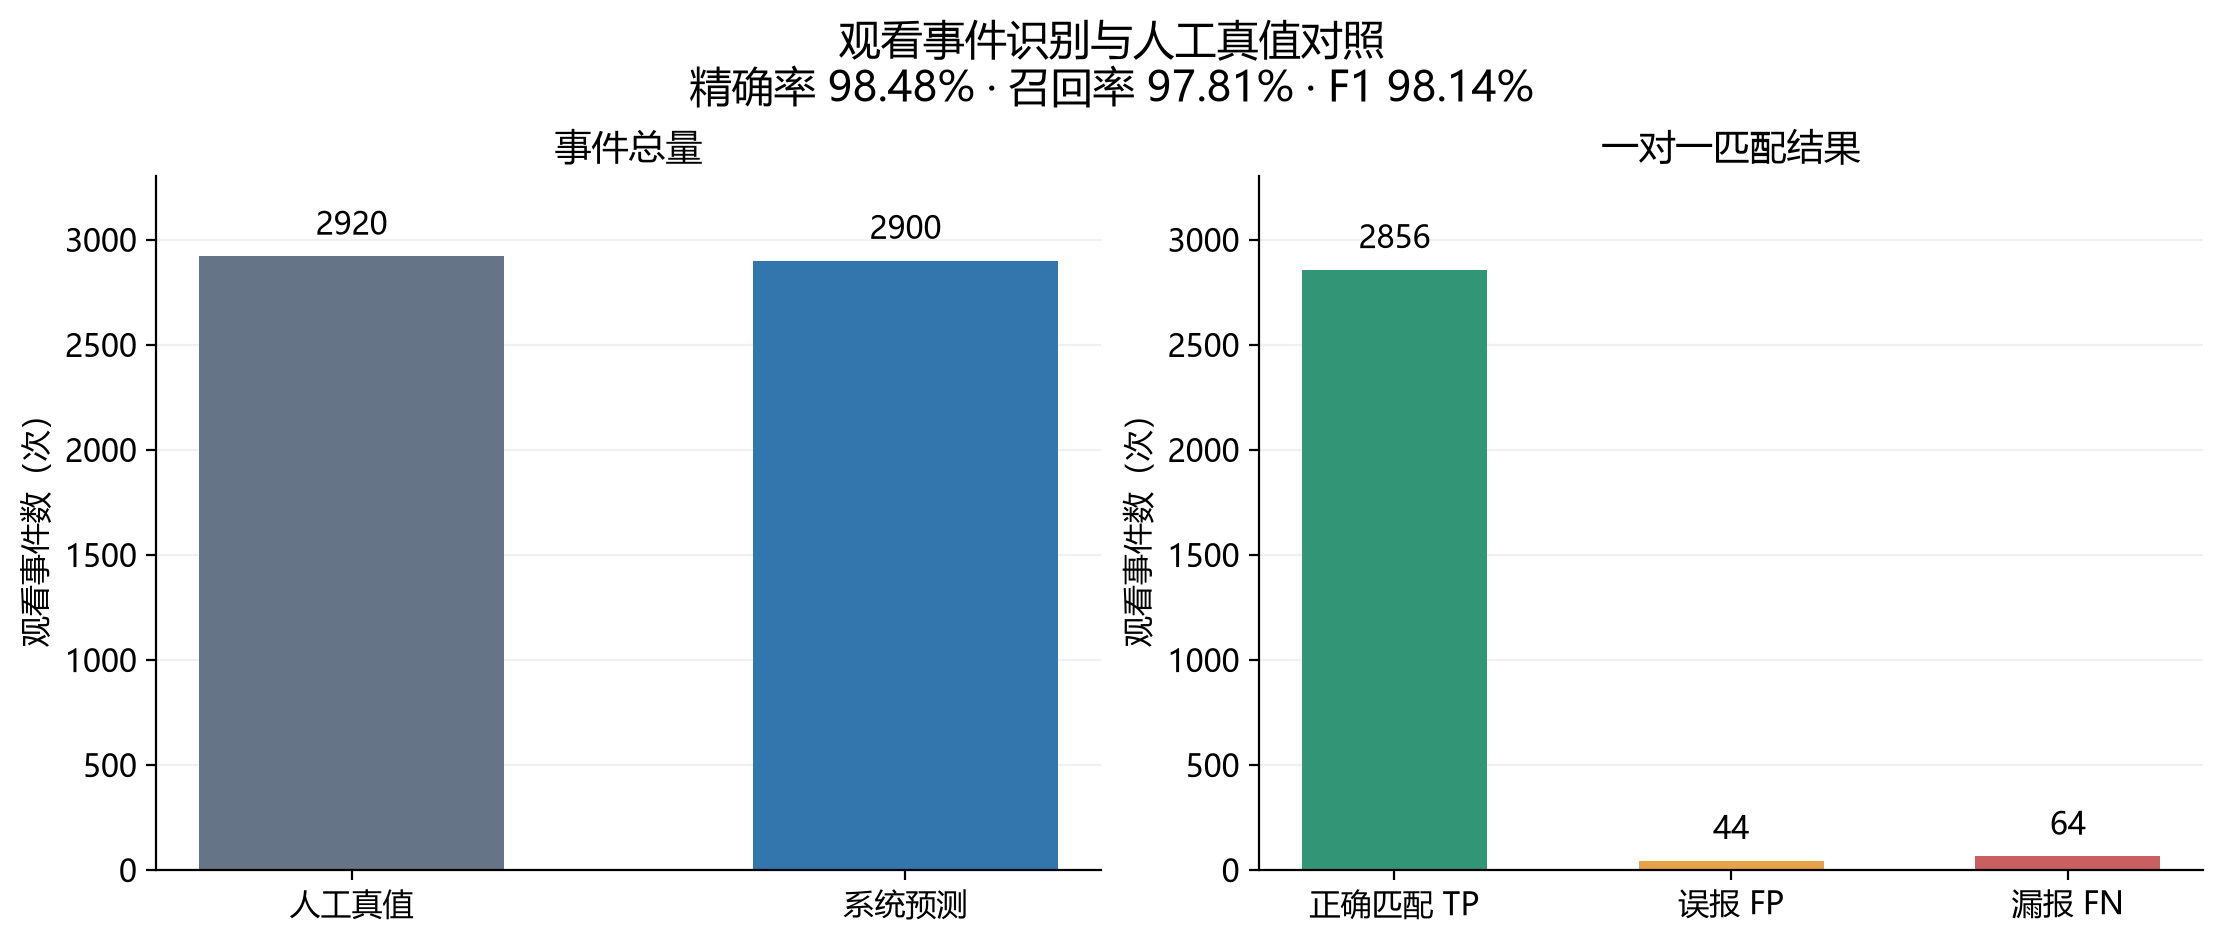
\includegraphics[width=\linewidth,height=0.66\textheight,keepaspectratio]{figures/chapter3/图3-2.png}
\caption{观看事件识别与人工真值对照}\label{fig:3-2}
\end{figure}

\subsubsection{相近观点与不同论据的端到端验证}\label{section:3.4.4}

第二个案例检验相同观点是否掩盖新增依据。用户在 09:10、09:18 及 10:05 依次接触 W-B/C/D，均围绕``当前招聘困难''。展示短语之外保留对象、时态、条件和论据，主题相似并非完全可比的充分条件。

W-B 正文呈现``某行业本月招聘岗位减少''，配图限定某城市应届岗位。W-C 字幕转述相同数据，画面显示同一匿名统计出处。双路检索召回 W-B，交叉判别确认范围相容，联合覆盖命中旧数据。W-C 与 W-B 归入同一观点并建立论据复用关系，但仍是两个实际浏览作品，不能因观点相同删除作品计数。

W-D 增加``部分岗位提高经验门槛''的材料，补充另一个行业条件及``区分岗位类型再投递''的建议。五维结果为事实新增、论据新增、条件新增、解释待定、行动新增。因片段不足以说明门槛变化的因果机制，解释维度保持待定。新增数据不自动转化为新增因果解释。

三条材料按同一观点展示时，作品数为 3、观点组为 1；其中 W-B 为首份材料，W-C 复用旧论据，W-D 包含新增依据。小时详情分别链接正文、关键帧或音频位置及过去历史。在 7 天案例序列中，20 个可分析作品有 16 个表达相近观点，占 80\%；其中 6 个包含新增论据，10 个为低增量重复。长期解释结合持续性、来源关系和阅读目的，不根据 80\%的集中度单独断言信息茧房。

\begin{figure}[htbp]
\centering
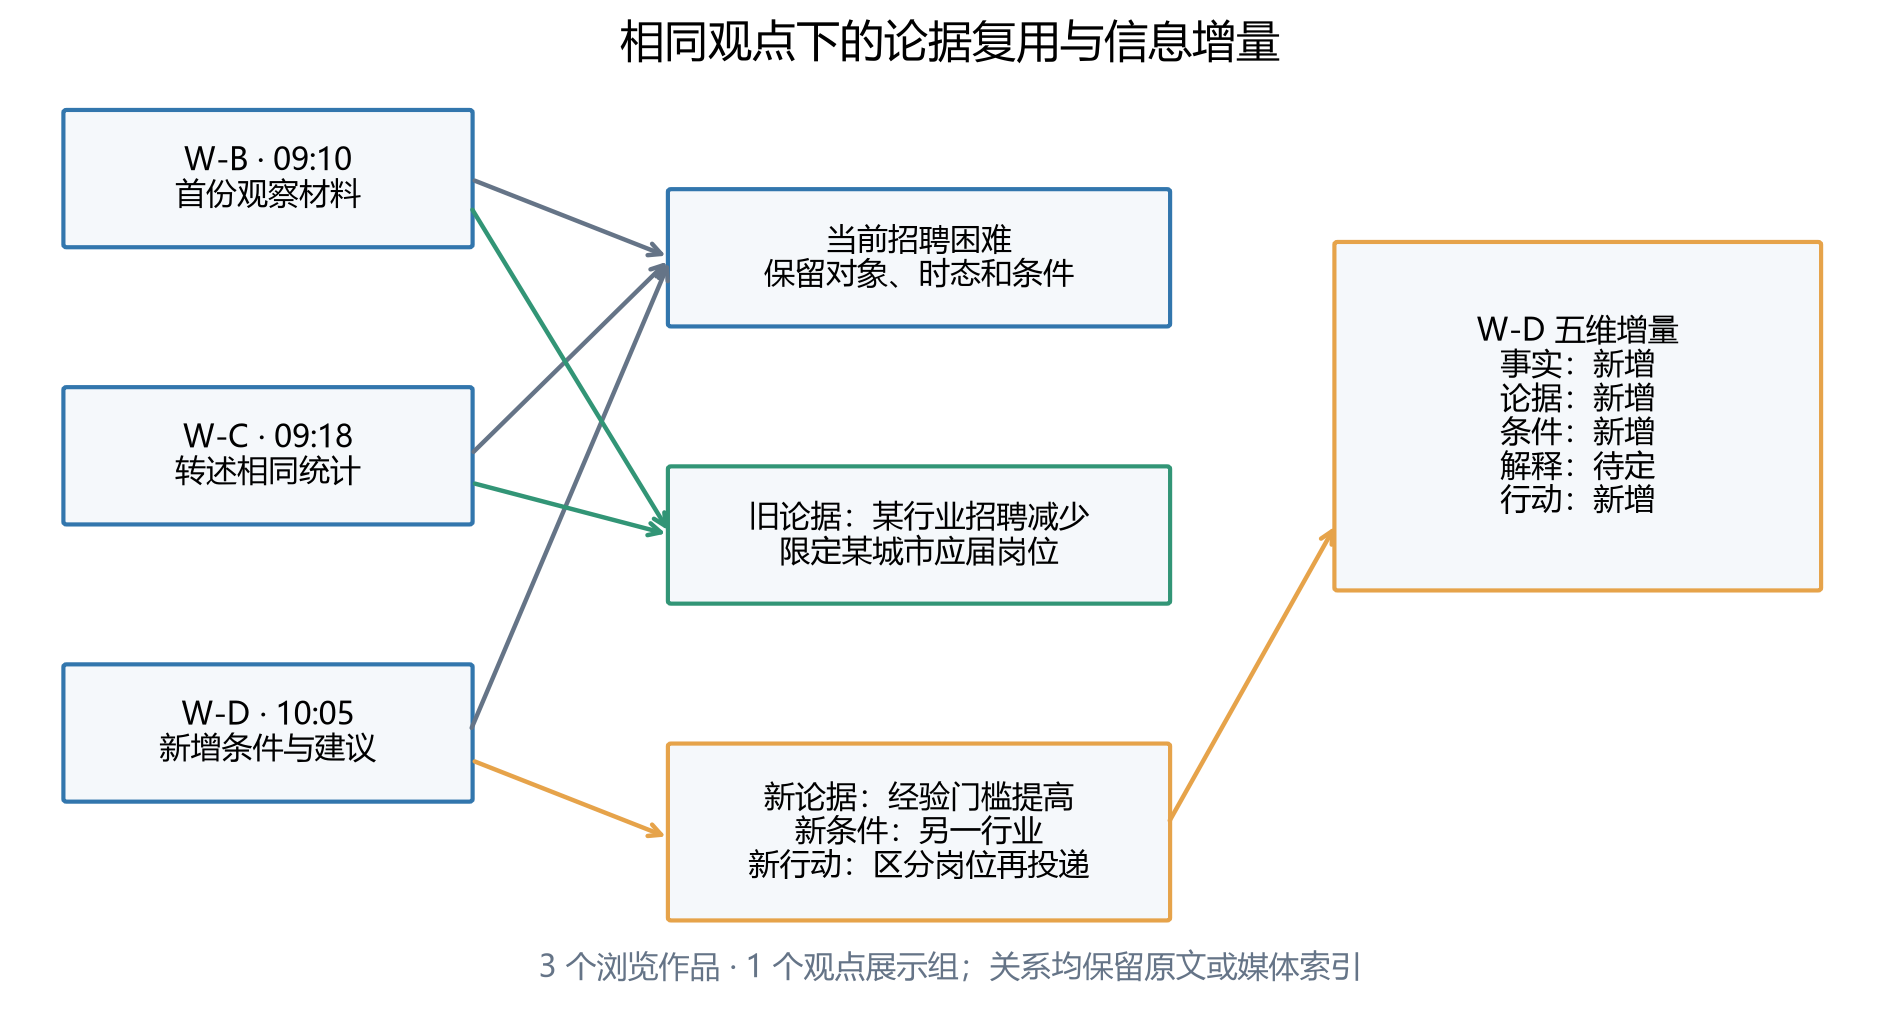
\includegraphics[width=\linewidth,height=0.66\textheight,keepaspectratio]{figures/chapter3/图3-3.png}
\caption{相同观点下的论据复用与信息增量}\label{fig:3-3}
\end{figure}

\subsection{多模态论证与个人历史增量评价}\label{section:3.5}

\subsubsection{论证联合理解}\label{section:3.5.1}

论证字段 macro-F1 分别计算主张、对象、立场、条件、论据与关系，再进行等权平均。实体跨度采用精确匹配，并另报告证据位置容差指标；主体归属在可判定样本上计算准确率，不用拒识样本扩大正确数。拒识覆盖率和已接受样本错误率共同报告。

\begin{longtable}[]{@{}
  >{\RaggedRight\arraybackslash}p{(\linewidth - 8\tabcolsep) * \real{0.1800}}
  >{\RaggedRight\arraybackslash}p{(\linewidth - 8\tabcolsep) * \real{0.2000}}
  >{\RaggedRight\arraybackslash}p{(\linewidth - 8\tabcolsep) * \real{0.2000}}
  >{\RaggedRight\arraybackslash}p{(\linewidth - 8\tabcolsep) * \real{0.2200}}
  >{\RaggedRight\arraybackslash}p{(\linewidth - 8\tabcolsep) * \real{0.2000}}@{}}
\caption{论证模型及消融结果}\label{tab:3-6}\tabularnewline
\toprule\noalign{}
方法 & 字段 macro-F1 & 主体归属准确率 & 证据定位 F1 & 已接受样本错误率 \\
\midrule\noalign{}
\endfirsthead
\toprule\noalign{}
方法 & 字段 macro-F1 & 主体归属准确率 & 证据定位 F1 & 已接受样本错误率 \\
\midrule\noalign{}
\endhead
\bottomrule\noalign{}
\endlastfoot
纯文字理解 & 0.752 & 0.854 & 0.731 & 12.8\% \\
文本、图像、音频直接拼接 & 0.787 & 0.881 & 0.768 & 11.3\% \\
移除对象条件化对齐 & 0.814 & 0.902 & 0.801 & 9.4\% \\
移除质量门控 & 0.819 & 0.910 & 0.805 & 10.6\% \\
移除证据定位监督 & 0.811 & 0.906 & 0.763 & 9.8\% \\
完整联合模型 & 0.846 & 0.934 & 0.862 & 7.1\% \\
\end{longtable}

完整模型字段 macro-F1 的 95\%整组自助法置信区间为{[}0.832,0.860{]}，主体归属准确率为{[}0.920,0.947{]}，均达到内部验收要求。已接受样本覆盖率为 88.4\%，其余保留证据不足或冲突状态；不能用仅接受高置信样本的指标代表全部输入准确率。

早期、中期、完整观察版本的字段 macro-F1 分别为 0.718、0.791 和 0.846。新增片段通过修订提高可判定程度，而没有把完整作品中的信息回填为早期已经观察的事实。跨模态对齐改善图中说明与语音转述的对象归属，质量门控主要减少低清图像和噪声音频引入的错误。残余错误包括反讽、多个主体同屏、隐含条件及 OCR 误识别。

\subsubsection{历史召回、关系判别与联合覆盖}\label{section:3.5.2}

历史评价先检索再判别，Recall@50 按每个当前材料所需的人工标注历史集合计算并宏平均；关系 F1 区分支持、矛盾、引用后反驳、条件变化和不可比状态。五维增量分别评价，不用主题相似度代替增量。

\begin{longtable}[]{@{}
  >{\RaggedRight\arraybackslash}p{(\linewidth - 6\tabcolsep) * \real{0.2500}}
  >{\RaggedRight\arraybackslash}p{(\linewidth - 6\tabcolsep) * \real{0.2500}}
  >{\RaggedRight\arraybackslash}p{(\linewidth - 6\tabcolsep) * \real{0.2500}}
  >{\RaggedRight\arraybackslash}p{(\linewidth - 6\tabcolsep) * \real{0.2500}}@{}}
\caption{历史比较方法对照}\label{tab:3-7}\tabularnewline
\toprule\noalign{}
方法 & Recall@50 & 五维增量 macro-F1 & 联合覆盖 F1 \\
\midrule\noalign{}
\endfirsthead
\toprule\noalign{}
方法 & Recall@50 & 五维增量 macro-F1 & 联合覆盖 F1 \\
\midrule\noalign{}
\endhead
\bottomrule\noalign{}
\endlastfoot
字面匹配与主题过滤 & 0.704 & 0.611 & 0.587 \\
单路语义向量 & 0.853 & 0.744 & 0.718 \\
双路召回、不使用交叉判别 & 0.927 & 0.776 & 0.751 \\
双路与交叉判别、仅单条历史覆盖 & 0.927 & 0.802 & 0.768 \\
完整双路与联合覆盖 & 0.941 & 0.837 & 0.858 \\
\end{longtable}

完整模型五维 F1 分别为事实 0.856、论据 0.872、条件 0.811、解释 0.824、行动 0.822，等权平均为 0.837。召回 Recall@50 为 0.941，达到 0.90 要求；五维 macro-F1 达到 0.80 要求。条件扩展和解释变化仍是主要误差来源，涉及省略语境时系统保留不确定状态。

联合覆盖将当前论据拆为可定位单元，并允许多个历史共同覆盖。完整方法较单条历史方法提高联合覆盖 F1 共 0.090，减少``旧论据分散在不同作品中，因此被当成新内容''的错误。对同观点新论据样本，模型保留观点重复与论据新增两个不同结果；对引用后反驳样本，引用命中不自动生成支持关系。

时间边界压力样本中，未来版本、同时间观察和后来补充的完整媒体均未进入早期历史候选；这是独立的工程约束，不由语义 F1 证明。信息增量只描述相对于已接触材料的新颖程度，不承担外部事实核查职责。

\subsubsection{误差案例与处置}\label{section:3.5.3}

案例一为快速切换中的过渡遮挡。用户在 0.8 秒内从视频 A 滑到 B，过渡帧仅有``关注''\,``评论''等公共控件，作者与标题暂不可见。按全文变化切分的方法会产生第三个作品。完整方法将其保留为未确认片段，取得稳定锚点后归入 B；如果未能取得，则不冒充已确认作品。计数仍有 44 次误报和 64 次漏报，主要说明极快切换与结构变化未完全解决。用户更正会撤销旧贡献并重算，不只修改列表文字。

案例二为引用后反讽。前半句为``大家都说`学历越高越没用'\,''，后半句为``那为什么不少岗位仍设置学历门槛''。早期片段仅有引用时，模型保留主体及立场不确定；后续音频抵达后，将引用归给被转述群体，作者表达修订为质疑。如果字幕漏识别否定词，质量门控保留模态冲突，不用一个模态的高置信掩盖冲突。该例展示迟到修订，不能替代测试集准确率。

案例三为隐含条件。相同``招聘困难''表达分别讨论应届生与有经验者，条件被截断时容易误判完全重复。补充片段后分别保存条件，撤销早期关系及其统计贡献，重放受影响图记忆；观察不足时不输出确定的零增量判断。

\begin{figure}[htbp]
\centering
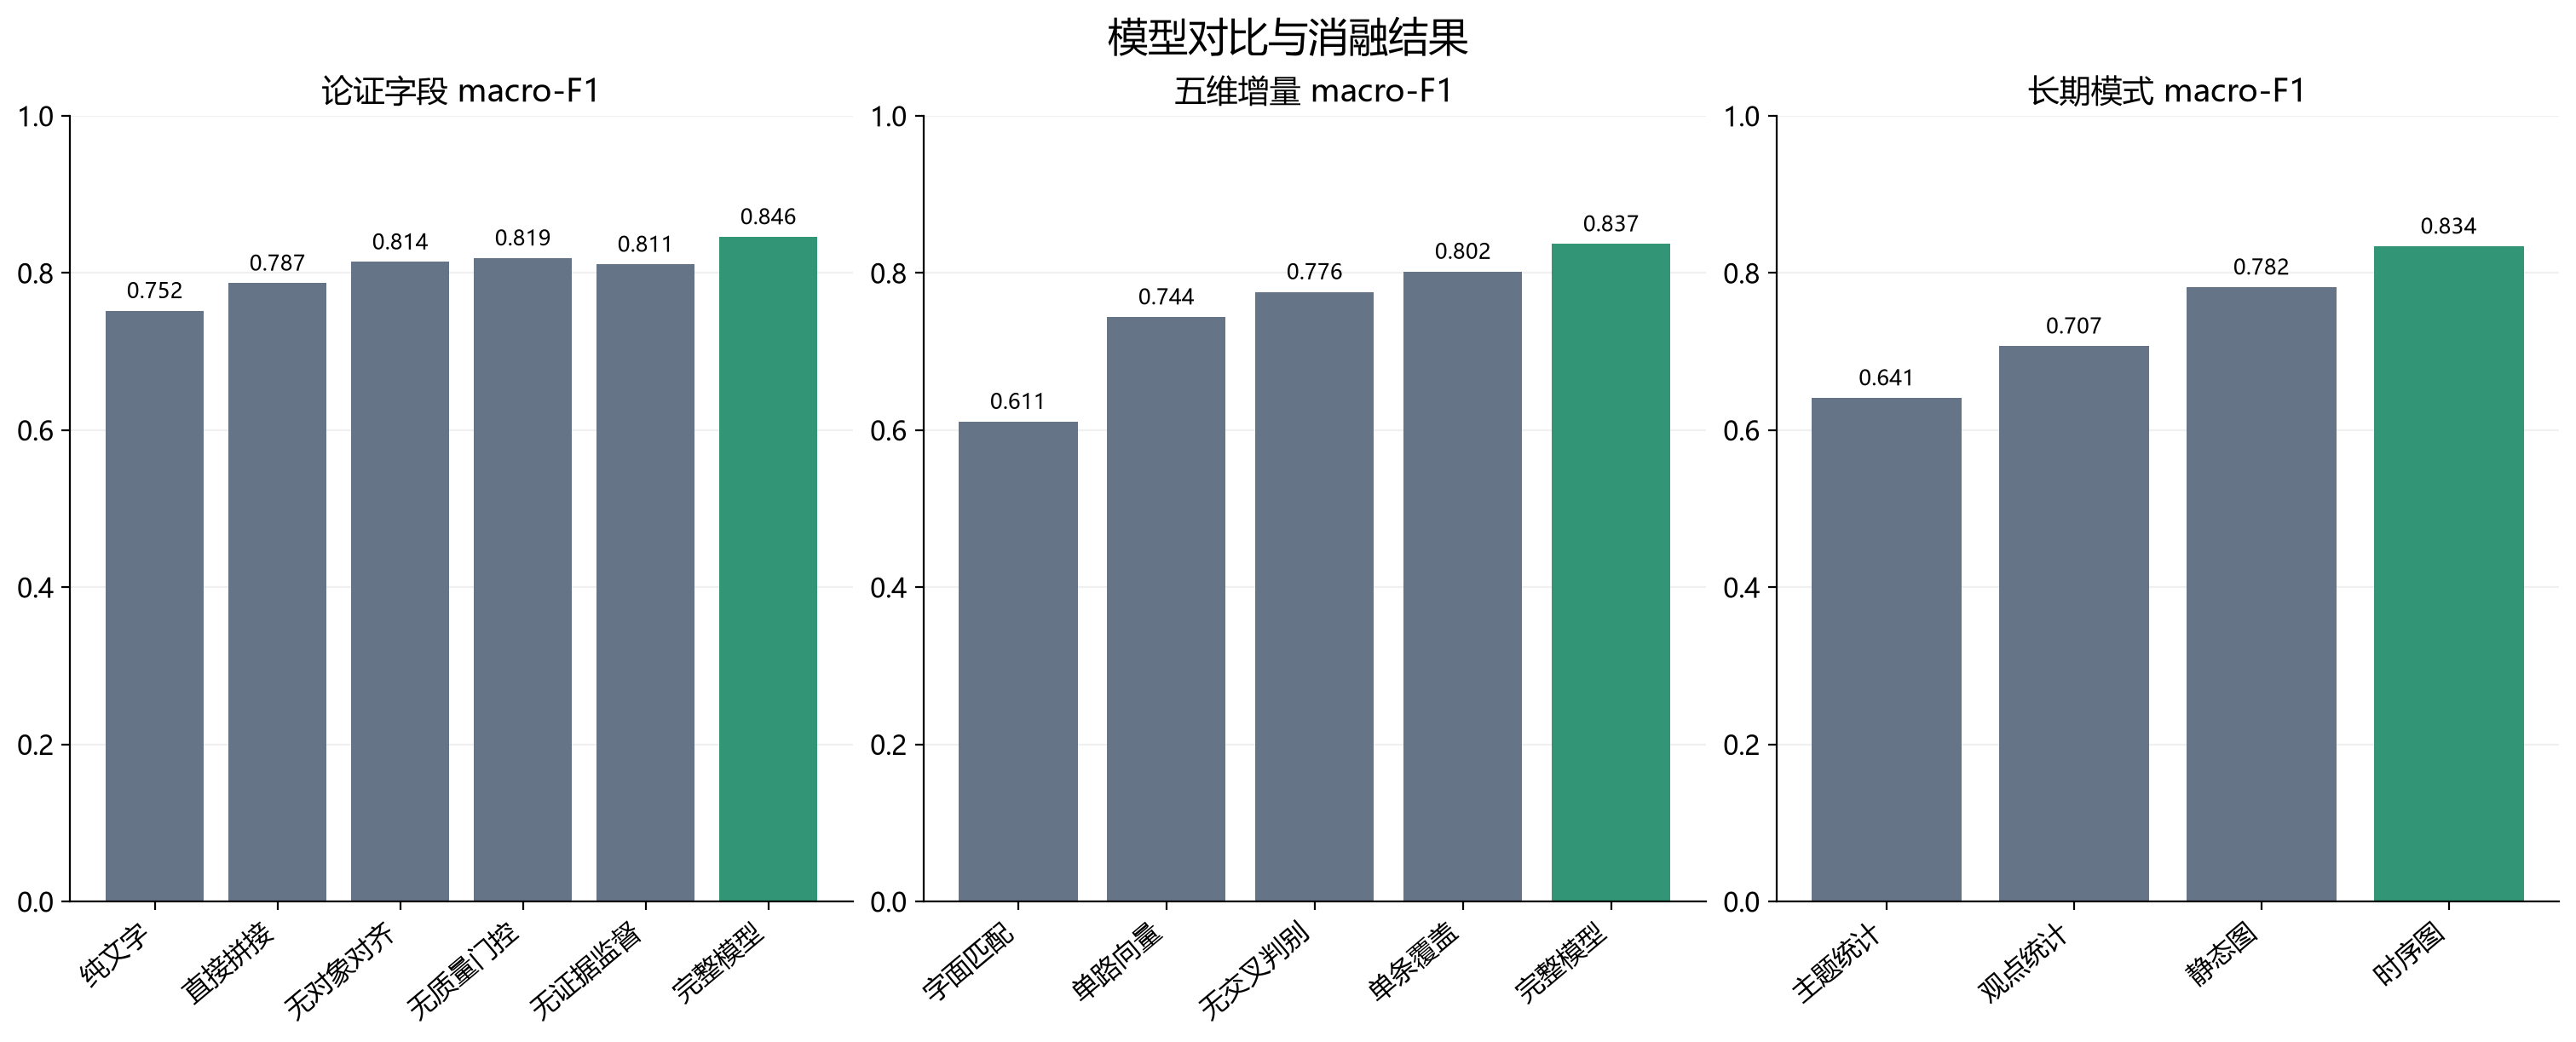
\includegraphics[width=\linewidth,height=0.66\textheight,keepaspectratio]{figures/chapter3/图3-4.png}
\caption{模型对比与消融结果}\label{fig:3-4}
\end{figure}

\subsection{时序论证图与长期接触模式分析}\label{section:3.6}

\subsubsection{对照设置及校准}\label{section:3.6.1}

长期评价采用主题统计、观点统计、静态图特征和带关系消息、时间编码与 GRU 记忆的时序论证图四种方法。测试标签覆盖持续低增量重复、正常专题学习、同源转载、不同立场接触和观察不足。误报率专门在正常专题学习窗口上计算，缺失窗口不作为低风险负例。

\begin{longtable}[]{@{}
  >{\RaggedRight\arraybackslash}p{(\linewidth - 8\tabcolsep) * \real{0.1800}}
  >{\RaggedRight\arraybackslash}p{(\linewidth - 8\tabcolsep) * \real{0.2000}}
  >{\RaggedRight\arraybackslash}p{(\linewidth - 8\tabcolsep) * \real{0.2000}}
  >{\RaggedRight\arraybackslash}p{(\linewidth - 8\tabcolsep) * \real{0.2200}}
  >{\RaggedRight\arraybackslash}p{(\linewidth - 8\tabcolsep) * \real{0.2000}}@{}}
\caption{长期接触模式对照结果}\label{tab:3-8}\tabularnewline
\toprule\noalign{}
方法 & 用户隔离 macro-F1 & 同用户未来 macro-F1 & 专题学习误报率 & 用户隔离 ECE \\
\midrule\noalign{}
\endfirsthead
\toprule\noalign{}
方法 & 用户隔离 macro-F1 & 同用户未来 macro-F1 & 专题学习误报率 & 用户隔离 ECE \\
\midrule\noalign{}
\endhead
\bottomrule\noalign{}
\endlastfoot
主题集中统计 & 0.641 & 0.662 & 23.8\% & 0.112 \\
观点分布统计 & 0.707 & 0.725 & 18.4\% & 0.086 \\
静态论证图及解释特征 & 0.782 & 0.805 & 10.7\% & 0.061 \\
完整时序论证图 & 0.834 & 0.858 & 6.4\% & 0.034 \\
\end{longtable}

ECE 采用 15 个等频置信桶，按桶内预测准确率与置信均值差的绝对值加权计算；温度校准在验证集完成，测试期不重新拟合。用户隔离 macro-F1 达到 0.80，ECE 低于 0.05；同用户未来结果单独反映早期个体背景的作用，不能替代新用户泛化能力。

在用户隔离协议中，移除历史增量、移除来源关系、移除时间编码与记忆后的 macro-F1 分别为 0.766、0.805 和 0.789，完整模型为 0.834。结果说明持续性和论据复用能够补充观点集中统计，跨平台不意味着来源必然独立，正常专题学习也不等于持续低增量重复。

\subsubsection{观察窗口与解释}\label{section:3.6.2}

3 天、7 天和 14 天窗口在用户隔离协议中的 macro-F1 分别为 0.758、0.812 和 0.834。短窗口能迅速定位集中浏览，但更容易混淆阶段性任务与持续重复；长窗口提供较稳定的历史依据，同时提高缺失记录管理要求。系统对有效覆盖不足的窗口输出观察不足状态，而不是依据低数据量生成确定风险分数。

面向用户的解释展示观点集中、低增量重复、旧论据复用、来源关系与持续天数，并连接相关作品和原文。模型估计是接触模式的校准概率，不是``认知受影响程度''的直接测量。专题学习误报仍有 6.4\%，因此报告结合用户阅读目的与阶段性任务说明，不采用单次高分强制干预。

\subsection{情绪诱因、角色与个人反馈评价}\label{section:3.7}

情绪模型围绕候选对矩阵、行列交互和角色链接开展评价；认知评价分支保留适用性与五级强度，生活处境和表达方式使用相应标签。个人反应校准仅使用自愿反馈，内容表达结果与自报结果分开存储和展示。

\begin{longtable}[]{@{}
  >{\RaggedRight\arraybackslash}p{(\linewidth - 8\tabcolsep) * \real{0.1800}}
  >{\RaggedRight\arraybackslash}p{(\linewidth - 8\tabcolsep) * \real{0.2000}}
  >{\RaggedRight\arraybackslash}p{(\linewidth - 8\tabcolsep) * \real{0.2000}}
  >{\RaggedRight\arraybackslash}p{(\linewidth - 8\tabcolsep) * \real{0.2200}}
  >{\RaggedRight\arraybackslash}p{(\linewidth - 8\tabcolsep) * \real{0.2000}}@{}}
\caption{情绪联合模型评价}\label{tab:3-9}\tabularnewline
\toprule\noalign{}
方法 & 情绪---原因配对 F1 & 角色跨度 F1 & 归属准确率 & 认知评价等级 MAE \\
\midrule\noalign{}
\endfirsthead
\toprule\noalign{}
方法 & 情绪---原因配对 F1 & 角色跨度 F1 & 归属准确率 & 认知评价等级 MAE \\
\midrule\noalign{}
\endhead
\bottomrule\noalign{}
\endlastfoot
共享编码、独立配对 & 0.704 & 0.731 & 0.827 & 0.83 \\
二维交互、不使用角色链接 & 0.757 & 0.768 & 0.866 & 0.72 \\
移除认知评价条件化 & 0.774 & 0.807 & 0.900 & 0.69 \\
完整联合模型 & 0.802 & 0.829 & 0.923 & 0.58 \\
\end{longtable}

完整模型配对 F1 超过 0.75。认知评价适用性 F1 为 0.871，生活处境 macro-F1 为 0.816，表达方式 macro-F1 为 0.834；等级 MAE 仅在维度适用且具备金标的样本上计算，未提及状态不编码为最低强度。隐含诱因、多持有者及讽刺表达仍产生错误，空诱因节点保留为未定位而不补造原因。

参与者回顾任务共安排每人每天 1 次、2,800 次，收到 2,240 次反馈，回应率 80.0\%，其中 2,100 次具备完整有效标签、140 次字段不完整，其余 560 次未回应。缺失反馈不作为``无焦虑''。在用户隔离测试的 360 次有效反馈上，内容表达直接映射个人反应的等级 MAE 为 0.92，经过独立校准为 0.74；时间隔离测试使用 420 次有效反馈，早期反馈个体适配后的 MAE 为 0.62。两个协议样本来自不同划分，指标不能拼接为总体效果。

该结果衡量模型与参与者自报的一致性，不是临床效度，也不证明浏览内容导致某种情绪。反馈可以撤回，撤回后重建受影响的校准状态和报告。

\subsection{异步处理与系统性能}\label{section:3.8}

\subsubsection{负载与统计范围}\label{section:3.8.1}

基础负载为 30 台逻辑在线设备，每台每分钟 20 个新事件，合计 10 个事件/秒。每轮预热 10 分钟后连续运行 60 分钟，共 36,000 个事件，重复 5 轮共 180,000 个事件。采用固定数据集片段回放，回放次数只用于负载测量，不增加自然作品样本规模。端到端时延从客户端发送起点测量，服务器排队与计算分别记录；公网不确定波动不纳入受控网络下的服务容量结论。

每轮测量接收确认、首个可用语义结果、完整分析、报告更新、GPU 利用率与各阶段队列。P95 先在每轮事件上计算，表中报告 5 轮 P95 的均值；吞吐按完成数量除以测量时长计算。模型完成时延包含队列、OCR/ASR 及后续历史和图更新，不能以快速接收确认替代。

\begin{longtable}[]{@{}
  >{\RaggedRight\arraybackslash}p{(\linewidth - 6\tabcolsep) * \real{0.2500}}
  >{\RaggedRight\arraybackslash}p{(\linewidth - 6\tabcolsep) * \real{0.2500}}
  >{\RaggedRight\arraybackslash}p{(\linewidth - 6\tabcolsep) * \real{0.2500}}
  >{\RaggedRight\arraybackslash}p{(\linewidth - 6\tabcolsep) * \real{0.2500}}@{}}
\caption{10 事件/秒基础负载结果}\label{tab:3-10}\tabularnewline
\toprule\noalign{}
指标 & 测量值 & 内部验收依据或解释 & 状态 \\
\midrule\noalign{}
\endfirsthead
\toprule\noalign{}
指标 & 测量值 & 内部验收依据或解释 & 状态 \\
\midrule\noalign{}
\endhead
\bottomrule\noalign{}
\endlastfoot
接收确认 P50/P95 & 118/286 毫秒 & P95≤500 毫秒，使快速浏览先得到记录状态 & 达标 \\
首个可用语义结果 P50/P95 & 0.91/2.18 秒 & 阶段结果与浏览并行，不阻塞客户端 & 通过 \\
完整模型分析 P50/P95 & 3.82/8.74 秒 & 独立报告精细理解尾延迟 & 通过 \\
完成后报告更新 P95 & 420 毫秒 & 统计更新不等待下一次浏览 & 通过 \\
事件级最终完成吞吐 & 10.00 事件/秒 & 到达与长期完成相匹配 & 达标 \\
待完成队列 P95 & 72 个事件 & 包含正在处理及排队的多阶段事件 & 通过 \\
每轮最后 10 分钟净积压变化 & −3 至+4 个事件 & 无持续增长，有限波动 & 达标 \\
单 GPU 平均利用率 & 72\% & 体现基础负载下的资源余量 & 通过 \\
\end{longtable}

各阶段饱和能力分别为初步理解 24、OCR 13、ASR 4.1、精细理解 5.4、历史比较 19、图更新 42 个任务/秒；相应基础到达率为 10、5、2、3、10、10 个任务/秒。OCR/ASR 等能力按各自任务定义测量，不能直接相加为系统作品吞吐。

\begin{figure}[htbp]
\centering
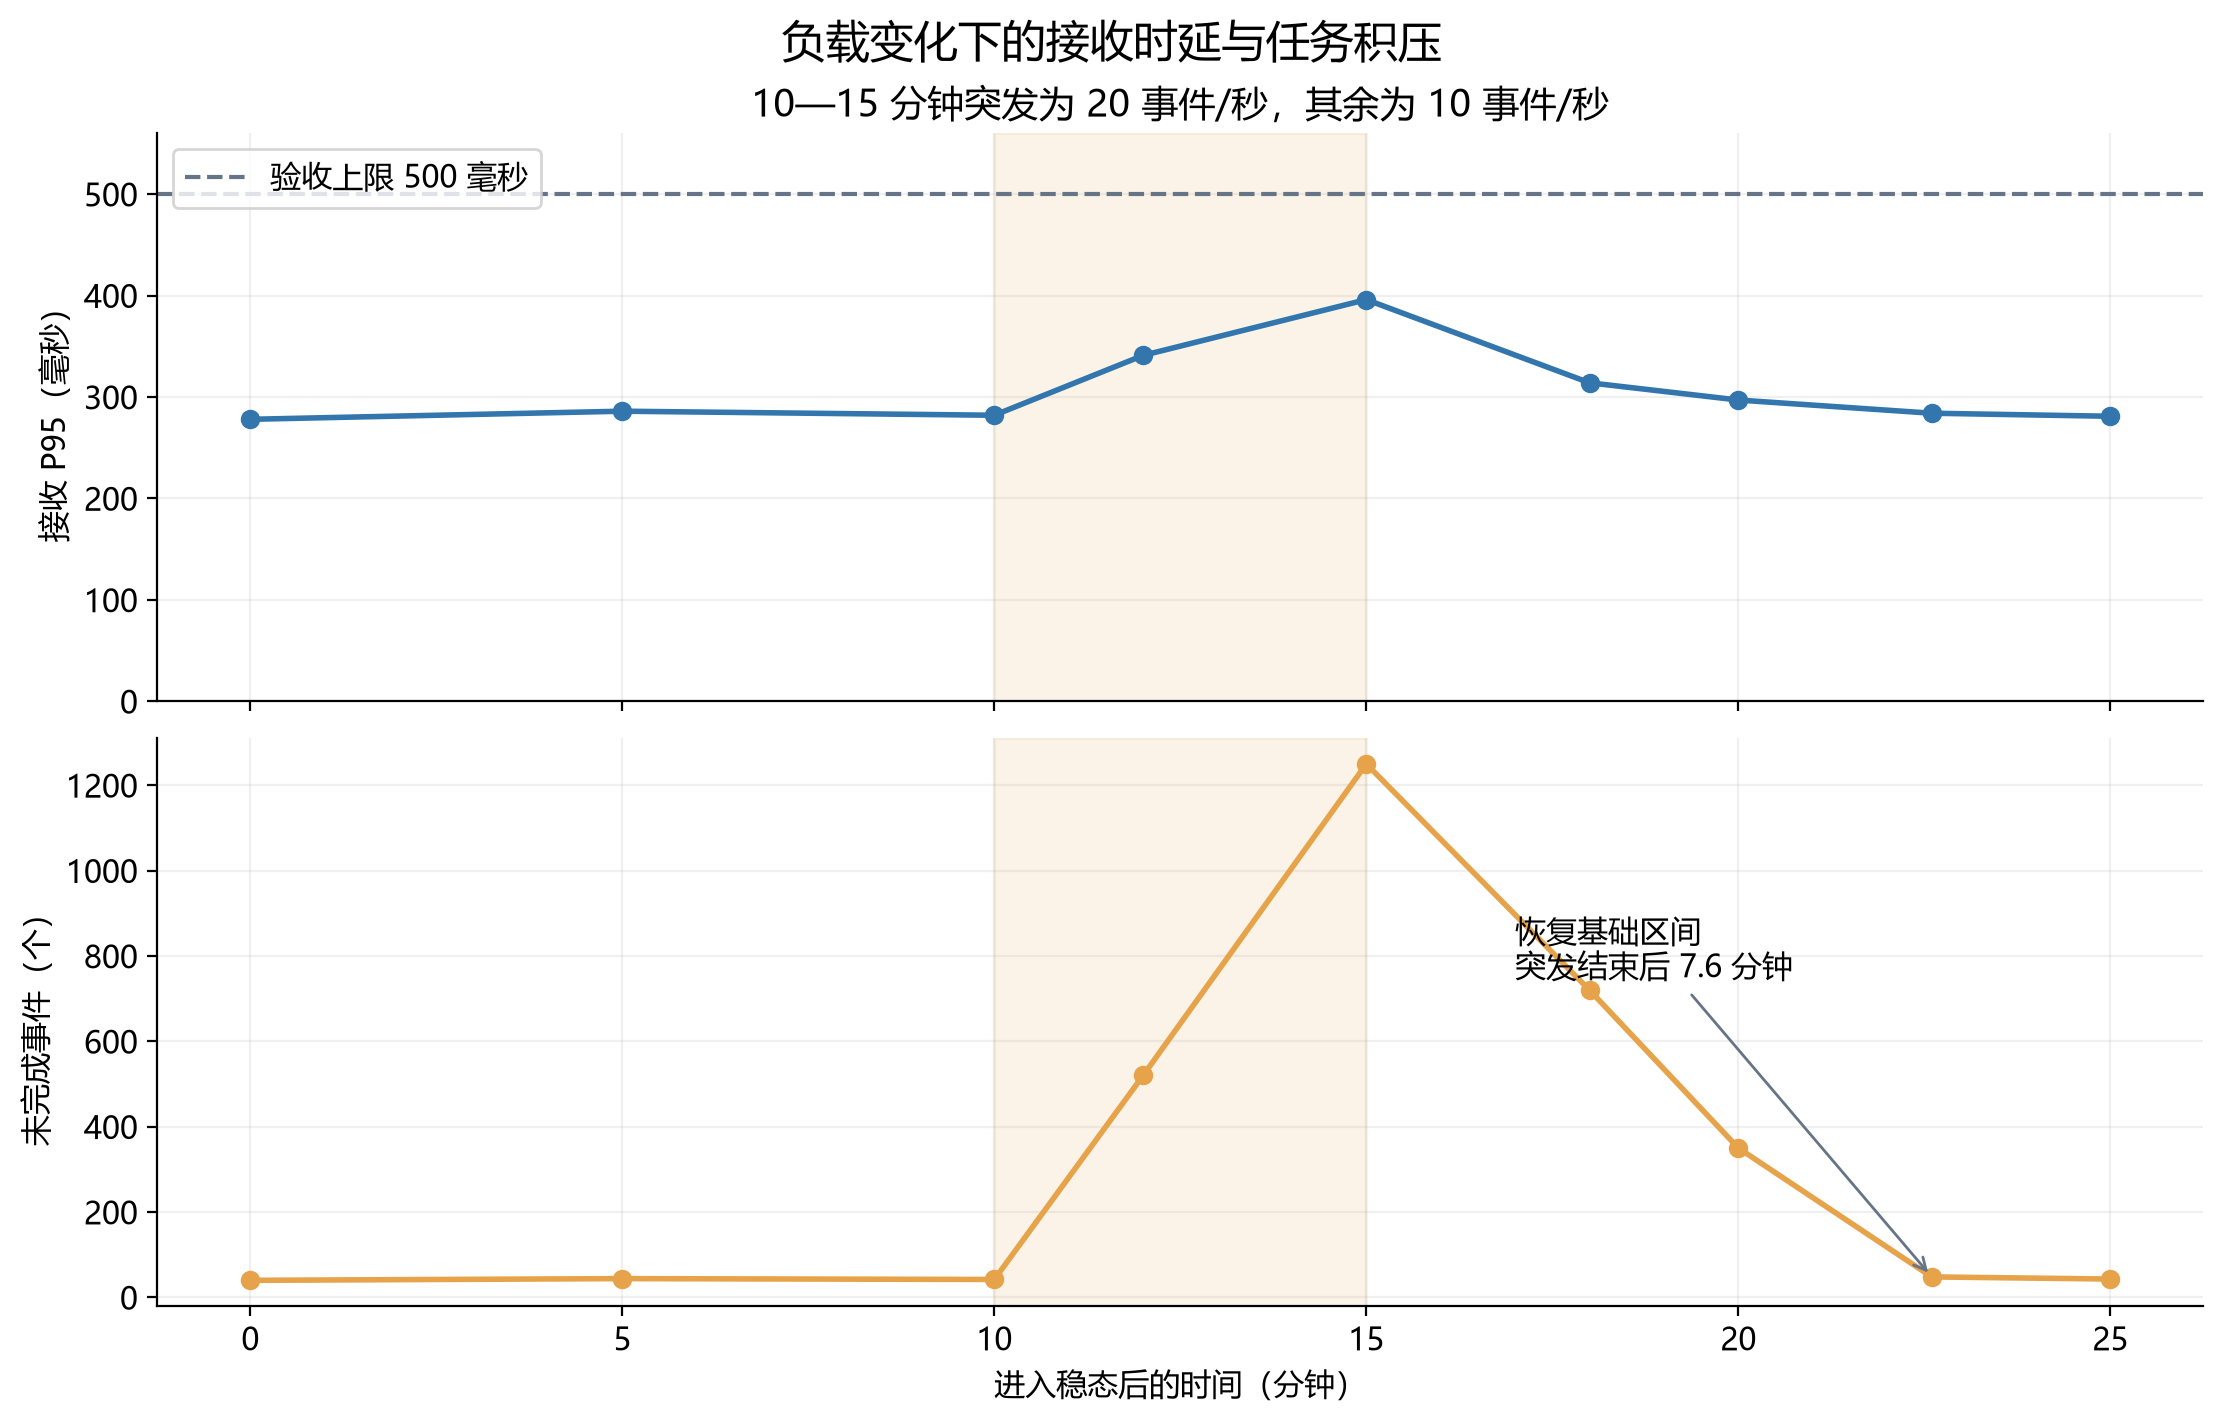
\includegraphics[width=\linewidth,height=0.66\textheight,keepaspectratio]{figures/chapter3/图3-5.png}
\caption{负载变化下的接收时延与任务积压}\label{fig:3-5}
\end{figure}

\begin{longtable}[]{@{}
  >{\RaggedRight\arraybackslash}p{(\linewidth - 6\tabcolsep) * \real{0.2500}}
  >{\RaggedRight\arraybackslash}p{(\linewidth - 6\tabcolsep) * \real{0.2500}}
  >{\RaggedRight\arraybackslash}p{(\linewidth - 6\tabcolsep) * \real{0.2500}}
  >{\RaggedRight\arraybackslash}p{(\linewidth - 6\tabcolsep) * \real{0.2500}}@{}}
\caption{突发负载及队列恢复过程}\label{tab:3-11}\tabularnewline
\toprule\noalign{}
时间（分钟） & 输入事件/秒 & 最近一分钟接收 P95（毫秒） & 未完成事件 \\
\midrule\noalign{}
\endfirsthead
\toprule\noalign{}
时间（分钟） & 输入事件/秒 & 最近一分钟接收 P95（毫秒） & 未完成事件 \\
\midrule\noalign{}
\endhead
\bottomrule\noalign{}
\endlastfoot
0 & 10 & 278 & 40 \\
5 & 10 & 286 & 44 \\
10，突发前 & 10 & 282 & 42 \\
12 & 20 & 341 & 520 \\
15，突发结束前 & 20 & 396 & 1,250 \\
18 & 10 & 314 & 720 \\
20 & 10 & 297 & 350 \\
22.6 & 10 & 284 & 48 \\
25 & 10 & 281 & 43 \\
\end{longtable}

图~\ref{fig:3-5}显示，突发负载结束后 7.6 分钟，未完成任务数量恢复至基础负载区间。曲线中的瞬时积压量与 5 轮基础负载测试的队列 P95（72）分别统计；较短的接收时延不代表精细分析无需排队。

\subsubsection{突发、恢复与端侧开销}\label{section:3.8.2}

持续 5 分钟输入 20 事件/秒时，资源受限阶段积压增加；恢复 10 事件/秒后，队列在 7.6 分钟内回到基础区间。系统未丢弃已经确认接收的事件，低质量或重复片段的跳过均记录原因。断网 60 秒后的端侧重传不重复计数，服务器重启后的未完成任务根据阶段与版本重入队列，恢复不依赖明文日志。

真机连续观察 30 分钟时，相对同内容浏览基线，新增电量消耗为 2.1 个百分点，设备表面温升增量为 1.8 ℃，前台丢帧率由 2.4\%升至 3.2\%。测试固定屏幕亮度、刷新率和网络，采用同设备配对实验，不能把两款不同手机的电量差作为采集服务开销。授权上传量在该混合负载下平均为 0.62 MB/事件，视频片段贡献较高，用户可以关闭媒体采集以减少流量，但报告同步降低相应观察覆盖。

\subsection{可验证机密计算与安全测试}\label{section:3.9}

\subsubsection{威胁模型及用例分类}\label{section:3.9.1}

外部服务域的攻击能力包括读取外部存储、修改报文、替换镜像、恢复旧快照和干扰消息顺序。客户端密钥管理、硬件隔离、证明信任根及获准服务构成可信计算基；客户端最新检查点有效保存是历史新鲜度判断的前提。终端完全失陷、未知硬件漏洞、访问时序完全隐藏和拒绝服务消除不属于已证明性质。

120 个场景按 12 类组织，每类 10 个参数化场景。Mock 模式运行全部状态机用例；其中 90 个证明、链路与状态场景另在真实 CPU 机密环境重复，60 个包含 GPU 设备与通信边界的相关场景再于 GPU 机密环境重复。场景重复执行不新增场景种类，也不以 Mock 结果替代硬件证明。

\begin{longtable}[]{@{}
  >{\RaggedRight\arraybackslash}p{(\linewidth - 6\tabcolsep) * \real{0.1600}}
  >{\RaggedRight\arraybackslash}p{(\linewidth - 6\tabcolsep) * \real{0.2800}}
  >{\RaggedRight\arraybackslash}p{(\linewidth - 6\tabcolsep) * \real{0.2800}}
  >{\RaggedRight\arraybackslash}p{(\linewidth - 6\tabcolsep) * \real{0.2800}}@{}}
\caption{安全测试结果与证明范围}\label{tab:3-12}\tabularnewline
\toprule\noalign{}
场景类型 & 注入输入或步骤 & 预期结果 & 结果及证明范围 \\
\midrule\noalign{}
\endfirsthead
\toprule\noalign{}
场景类型 & 注入输入或步骤 & 预期结果 & 结果及证明范围 \\
\midrule\noalign{}
\endhead
\bottomrule\noalign{}
\endlastfoot
正常握手 & 正确挑战、公钥、清单与证明链 & 建链、密钥确认、授权后执行 & 10/10 通过；证明允许流程可用 \\
挑战重用 & 使用旧挑战或重放证明 & 放行谓词拒绝，存储密钥不释放 & 10/10 拒绝；验证本次会话新鲜度 \\
公钥替换 & 替换任一临时公钥 & 转录绑定或密钥确认失败 & 10/10 拒绝；验证端点绑定 \\
测量与清单不符 & 修改镜像、模型摘要、工具权限或调试策略 & 策略不匹配，不进入授权阶段 & 10/10 拒绝；依赖加载器正确校验 \\
密文与对象篡改 & 修改密文、关联数据、对象结构版本 & AEAD 或对象校验失败 & 10/10 拒绝；不证明语义内容真实 \\
序号重放 & 旧 seq 报文再次发送 & 重放拒绝，事件状态不重复推进 & 10/10 拒绝；业务重试另用幂等标识 \\
用途与方向混用 & 交换上传/下载或数据/控制密钥上下文 & 认证失败 & 10/10 拒绝；验证四类密钥分离 \\
旧快照恢复 & 宿主机提供旧版本及旧对象根 & 与最新客户端锚点不符，转入重同步 & 10/10 拒绝；要求最新锚点未丢失 \\
确认前后掉线 & 在两阶段提交各边界切断连接 & 待提交不冒充已提交，凭锚点续传 & 10/10 状态一致；不承诺网络可用性 \\
越权与缓存串用 & 用户交叉请求、标识复用及会话切换 & 拒绝跨用户对象与图记忆访问 & 10/10 拒绝；检查内存、索引与队列 \\
删除及依赖重放 & 删除旧事件、论据或反馈 & 清理依赖闭包，重建报告与记忆 & 10/10 通过；密码销毁另核验密钥副本 \\
授权撤回及 GPU 边界 & 会话撤权、GPU 证明无效或链路不合策略 & 停止对应任务、清理缓存或禁止 GPU 执行 & 10/10 通过预期拒绝/清理行为 \\
\end{longtable}

恶意页面中的指令性文字只进入分析数据层。附加 200 条指令注入探针覆盖诱导外联、修改工具权限与跨用户查询，均未产生未授权工具调用；该结果只覆盖探针集合，不能推导模型对任何新型注入都免疫。

\subsubsection{历史提交、删除与可追溯性}\label{section:3.9.2}

客户端检查点包含用户标识、密钥代次、提交版本、Merkle 根及前驱摘要。服务器准备状态后回读对象，客户端原子保存检查点再确认；恢复先核对根和最新确认版本，再在可信边界内解密。客户端已保存而服务端未收到确认的事务能够凭检查点完成；尚未保存的候选版本保持待提交。恢复用例未出现旧快照被误当作最新已确认状态。

删除沿依赖闭包移除转写、向量、关系和缓存，并按固定模型版本从有效检查点重放保留事件。日报、历史比较和时序记忆同步修订，多来源摘要按保留材料重建。涉及密码学销毁时回收对应密钥代次及受管理备份，已经导出到用户终端或第三方位置的报告不宣称能够被远程撤回。

日志检查未发现原文、提示模板输入、向量或报告明文落入外部日志。宿主机可见任务大小与访问时间等元数据仍存在，合并请求及分级填充降低粒度但不实现完全不可观察。硬件与客体运行时均属于需要持续维护的安全前提，证明有效不等于分析结论必然正确。

\subsubsection{机密执行开销}\label{section:3.9.3}

在同一 NCC40ads H100 v5 硬件、同一模型和同一回放序列上比较常规与机密模式，不采用跨云 A10G 与 H100 的时间差。完整分析平均时延分别为 3.40 秒与 3.78 秒，增量为 11.18\%；接收确认 P95 由 254 毫秒增至 286 毫秒，增量为 12.60\%。单次会话证明与建链 P95 为 1.34 秒，不计入已建链事件接收时延；增量状态提交 P95 为 168 毫秒，1 GB 历史恢复 P95 为 2.84 秒。

开销来自证明、受保护传输、加密对象与检查点提交。会话复用摊薄证明成本，但会话过期、版本切换及重启均重新证明。上述相对开销只适用于本章规定输入和硬件，不能外推为全部模型与实例的固定开销。

\begin{figure}[htbp]
\centering
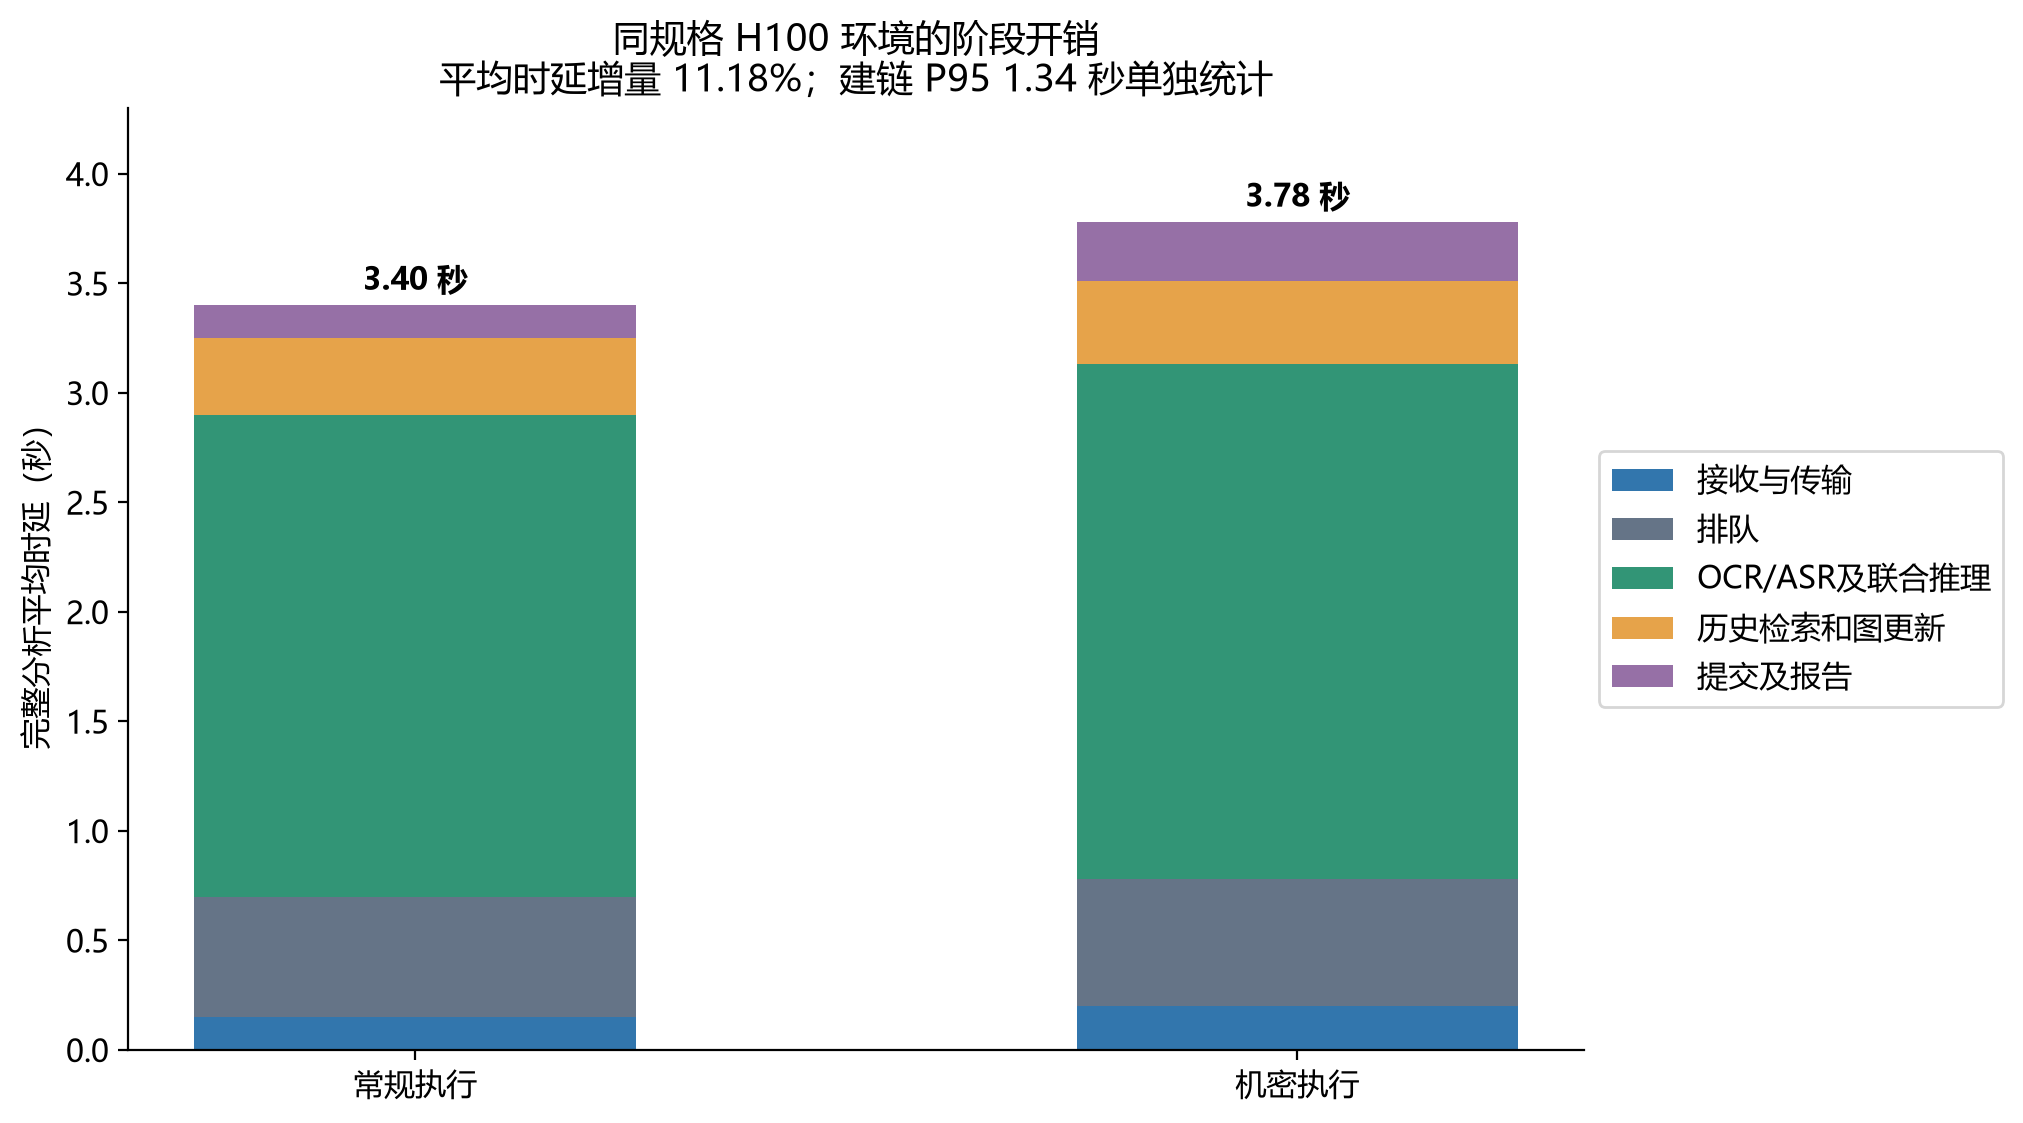
\includegraphics[width=\linewidth,height=0.66\textheight,keepaspectratio]{figures/chapter3/图3-6.png}
\caption{常规与机密执行的阶段开销}\label{fig:3-6}
\end{figure}

\subsection{复赛新增协同API路径的独立验收范围}
新增协同API路径的测试与前述初赛实验分别记录。协议回归涵盖会话签名、载荷认证、历史版本和哈希匹配、失败不推进状态及重试处理；这些离线用例不能替代硬件远程证明或商业模型准确率评价。Room v10新增按日期及议题组织的物化统计，并以事件贡献和事实身份索引维护删除、重分析及跨日去重。预热后的摘要查询、首次回填和包含原文排版的完整PDF生成必须分别计时，不能用摘要查询时间宣称完整报告生成低于15毫秒。

商业API与本地轻量化基准的事实合并F1、情绪引导F1、误报率及端到端P50/P95，需要在相同保留测试集、固定模型版本与网络条件下重新测量。本轮代码与离线协议验收不提供这些新实验结果，故不填入预设的提升幅度或亚秒延迟。新版Android信息盲区、原文对照及管理端攻防截图仅在实际运行后采集，不以示意图冒充实机结果。详细执行记录见仓库\texttt{BUILD\_VALIDATION.md}及\texttt{docs/R3\_FINAL\_ITERATION\_PLAN.md}。

\subsection{验收依据、结果分析与章节小结}\label{section:3.10}

\subsubsection{内部验收标准及达标情况}\label{section:3.10.1}

\begin{longtable}[]{@{}
  >{\RaggedRight\arraybackslash}p{(\linewidth - 8\tabcolsep) * \real{0.1600}}
  >{\RaggedRight\arraybackslash}p{(\linewidth - 8\tabcolsep) * \real{0.2500}}
  >{\RaggedRight\arraybackslash}p{(\linewidth - 8\tabcolsep) * \real{0.2500}}
  >{\RaggedRight\arraybackslash}p{(\linewidth - 8\tabcolsep) * \real{0.2500}}
  >{\RaggedRight\arraybackslash}p{(\linewidth - 8\tabcolsep) * \real{0.0900}}@{}}
\caption{核心验收结果}\label{tab:3-13}\tabularnewline
\toprule\noalign{}
项目 & 内部阈值 & 本章结果 & 阈值设置依据 & 结论 \\
\midrule\noalign{}
\endfirsthead
\toprule\noalign{}
项目 & 内部阈值 & 本章结果 & 阈值设置依据 & 结论 \\
\midrule\noalign{}
\endhead
\bottomrule\noalign{}
\endlastfoot
作品计数 & P、R 均≥95\% & 98.48\%、97.81\% & 同时限制误拆分和漏记，避免只追求单侧指标 & 达标 \\
可见停留 & MAE≤2 秒 & 1.12 秒 & 降低快速切换时区间误差，区别实际阅读估计 & 达标 \\
幂等、修订、隔离 & 指定工程用例全部通过 & 无违反预期的状态贡献 & 重复上传和越权不应依靠概率容忍 & 通过 \\
论证字段 & macro-F1≥0.80 & 0.846 & 控制小类别退化，支持结构化证据回看 & 达标 \\
主体归属 & 准确率≥0.90 & 0.934 & 限制引用者与被引述者混淆 & 达标 \\
历史召回 & Recall@50≥0.90 & 0.941 & 降低漏检旧依据导致的虚假新增 & 达标 \\
五维增量 & macro-F1≥0.80 & 0.837 & 分开检查事实、论据、条件、解释与行动 & 达标 \\
长期模式 & macro-F1≥0.80、ECE≤0.05 & 0.834、0.034 & 平衡模式区分与概率可信程度 & 达标 \\
情绪---原因 & 配对 F1≥0.75 & 0.802 & 考虑跨片段配对难度，避免只输出情绪词 & 达标 \\
安全约束 & 定义的恶意用例全部拒绝 & 全部达到预期拒绝/隔离行为 & 放行前提与认证检查属于硬约束 & 通过 \\
基础容量 & 10 事件/秒；接收 P95≤500 毫秒；积压不持续增长 & 286 毫秒；完成 10.00 事件/秒；队列稳定 & 对应 30 设备快速浏览场景与异步交互 & 达标 \\
\end{longtable}

这些阈值是本项目的内部验收约定，来源于业务约束、漏检后果和交互目标，不是行业统一标准。阈值在查看测试结果之前冻结，不能在测试后通过降低标准得到达标结论。模型仍存在不确定与误差，因此通过验收不意味着所有输入均可分析。

\subsubsection{综合分析}\label{section:3.10.2}

采集层通过作品与事件分离减少重复计数，统计层通过区间并集和修订替换避免时长累加失真。多模态理解将观点组织为具有对象、立场、条件和论据的结构，证据定位与质量门控提高可解释性。历史联合覆盖能够处理旧依据分散在多个作品中的情况，使同观点新论据与低增量重复得到不同结果。

时序论证图相对于主题统计降低正常专题学习的误报，表明持续性、信息增量与来源关系是必要补充；情绪角色和认知评价分支减少内容表达与人物归属混淆。机密计算测试验证了规定威胁模型下的执行主体、通道与历史状态约束，但没有扩大为绝对隐私或模型真实性保证。

剩余改进集中在平台页面结构变化、极快切换、隐含条件、反讽、多主体归属和长尾议题。长期分析还受到观察覆盖和参与者反馈缺失影响。系统通过拒识、覆盖说明、证据回看与用户更正处理这些边界，报告的用途是支持个人审视信息环境，而不是替用户作出认同判断或心理诊断。

\subsubsection{本章小结}\label{section:3.10.3}

本章建立了与技术路线对应的分层测试体系，完成作品采集、阅读估计、跨模态论证、个人历史增量、时序图、情绪建模、异步处理和可信执行评价。核心模型指标达到内部标准，基础负载下接收和处理保持稳定，协议与状态用例满足规定约束。实验同时保留误差、拒识与未知范围，使工程达标、语义效果和安全边界分别得到解释。

% 第四章正文，直接编辑本文件。
\FloatBarrier\clearpage

\section{创新性说明}\label{chapter:4}

第一章将信息茧房的个人防护困难界定为``难以察觉、难以定位和难以核查''，第二章围绕这一困难给出了从浏览观测到认知体检报告的完整系统设计。本章在此基础上讨论作品的创新性。讨论遵循两个原则：其一，每项创新均对应第一章所分析的具体不足，说明现有做法为何不够、本作品改变了什么；其二，创新判断以可检验的设计差异为限，相关机制的实际作用由第三章设置的对照与消融实验分别验证，本章不作超出实验范围的效果断言。作品的四项研究任务分别对应内容内部的语义理解、内容之间的信息增量、浏览序列中的长期模式和持续分析的可信执行，本章 4.2、4.3、4.4 和 4.6 节分别讨论这四项任务的方法与系统创新，4.1 节讨论贯穿其间的问题定义创新，4.5 节讨论情绪分析的辅助方法创新，4.7 节汇总各项创新及其与现有方案的区别。

\subsection{问题定义创新}\label{section:4.1}

\subsubsection{可核查的个人浏览分析}\label{section:4.1.1}

既有研究为理解信息同质化提供了重要基础，但其分析单位与本作品面对的问题存在层次差异。传播结构研究比较平台之间用户互动的同质性\cite{ref1}，接触研究区分潜在接触、实际展示与用户点击\cite{ref3}，干预研究考察接触结构变化与态度后果的关系\cite{ref5}，国内研究则通过问卷讨论媒介使用与信息茧房指标的关联\cite{ref6}。这些工作的对象分别是群体、平台环节或自我报告，均不能回答个人层面的具体问题：某一位用户在一段时间内反复接触了什么观点，这些观点依赖哪些材料，后续内容是否补充了新的依据。

本作品的第一个创新在于把分析对象明确界定为个人授权范围内可观察、可核查的浏览经历。系统不要求掌握平台完整的社交网络，也不依赖用户事后回忆，而是以带时间索引的浏览记录为输入，将观点、论据与接触过程组织为结构化记录，并使每项结论能够回到具体片段核查。这一对象选择同时改变了结果形式：现有数字健康工具以应用时长和打开次数帮助用户发现时间分配问题\cite{ref2}，而本作品补充认知层面的解释，使同样一小时的浏览，``比较资料形成认识''与``重复接触缺少新依据的相同判断''能够被区分开来。分析的落点也由``用了多久''转向``接触了什么、依据是否增加''。

\subsubsection{以信息增量判别重复}\label{section:4.1.2}

识别同质化需要先回答``什么样的重复值得关注''。主题集中本身常对应合理的信息需求：求职期间集中研究岗位要求、升学期间集中比较院校政策，都是正常且有益的阅读。若以主题占比或观点一致性作为判别依据，持续深化的专题阅读将被误判为茧房。本作品提出以实质信息增量为核心判别线索，将其界定为新内容相对于个人此前已观察同议题历史所增加的事实、证据、限定条件、解释、反例或可执行建议，并进一步细分为事实、论据、条件、解释与行动五个维度。相同结论可以由新的数据和条件支撑，不同措辞也可能只是转述同一材料；只有同时考察观点与依据两层关系，才能区分``相同观点获得新依据''与``相同观点反复换写''。观点重复、信息增量与时间持续性三者结合，作为判别低增量同质接触的依据，补充面向个人的时长统计和单一主题分析。

\subsubsection{接触与认同的分析边界}\label{section:4.1.3}

本作品在定义阶段即明确了分析不能做什么，并将这些限制落实为系统机制而非口头声明。内容出现在屏幕上、用户可能重点阅读、用户认同其中判断，是三个不同层次，系统评估可观察接触结构，并以带置信度的行为线索估计阅读投入，不据此推断用户认同，记录中始终保留这种区分；内容中的焦虑表达与用户自身的焦虑状态分离，后者只能来自用户自愿提供的反馈；信息增量不直接代表事实真实性或个人知识增长；娱乐内容与观点型内容采用不同的解释方式，不因缺少知识增量而作负面评价。这些边界使报告始终是``用户审视自身信息环境的材料''，而不是对个人心理或认知状态的诊断。相比给出笼统风险分数的做法，将分析边界、未知比例和``证据不足''状态列为系统的正式输出，是本作品在问题定义上的具体差异。

\subsection{多模态观点理解创新}\label{section:4.2}

\subsubsection{已观察片段边界建模}\label{section:4.2.1}

现有立场检测与论证挖掘研究以完整、静态的文本为单位。SemEval-2016 立场检测任务针对给定目标的完整推文判断立场\cite{ref8}，IAM 在完整文档上联合抽取主张、立场与论据\cite{ref13}，T-MAD 等多模态立场方法假设相关模态均已获得\cite{ref14}。真实浏览场景不满足这些假设：用户可能只看视频开头数秒，画面文字可能属于受访者而非作者，观点可能在后续口播中被反驳，各模态还可能分别缺失。将不完整片段按完整内容处理，正是混同讨论对象、发言主体与实际立场的根源。

本作品提出已观察多模态前缀的建模方式（定义 2-1，式 2-1、2-2），按片段首次被观察到的时间组织模型输入，使分析范围始终等于用户实际接触的范围，未被观察的内容不进入接触记录。在此基础上，论证单元统一记录讨论对象、表达主体、主张、论据、适用条件、单元间关系及证据索引，正文与评论分别建立单元并保留父项关系。由此，``用户看到了什么''成为模型的形式化输入条件，后续的历史比较与时序分析均建立在这一范围之上。

\subsubsection{目标对齐与质量门控}\label{section:4.2.2}

跨模态理解的常见做法是拼接各模态表示后统一分类，模态冲突在这种结构中容易被掩盖。本作品采用目标条件的跨模态对齐：围绕当前讨论对象分别查询文字、画面与音频词元，对齐过程加入媒体时间距离与画面空间关系偏置（式 2-3 至 2-5），再以对象相关性、识别质量、画面清晰度与片段覆盖状态为输入进行质量门控（式 2-6 至 2-8）。对象条件决定``应关注哪些片段''，质量门控决定``这些片段各占多大比重''，二者分工明确。当字幕与口播真实存在分歧时，系统输出两者的表达内容及冲突关系，而非强行融合为单一立场；观点归属、证据定位与充分度估计由联合损失共同训练（式 2-15 至 2-19），各自保留中间结果以支持逐项消融检验。对真实分歧的保留和对各机制贡献的可分离评价，是本方法相对于端到端融合方案的两点具体改进。

\subsubsection{可修订理解与双层证据}\label{section:4.2.3}

连续浏览中，理解结果必须能够随新片段到达而更新。本作品为每个字段独立估计证据充分度，区分``可输出''与``证据待补充''两种状态（式 2-13、2-14），使模型可以先呈现已确定的主张、暂缓不确定的归属，待补充片段到达后按版本修订。增量更新以受影响的对象和论证单元为范围，字段级差异向后传递至历史比较与图谱模块，旧版本保留用于追溯。与之配合的是论据与证据索引的双层记录：论据是原文用于支持判断的材料，证据索引是系统抽取该字段所依据的原文位置，两层关系分别保存。前者使历史比较能够检查材料层面的重复，后者使用户能够核查模型判断的出处。按此设计，每一项语义判断都附带出处，每一次修订都保留轨迹；可解释性不再是事后附加的展示功能，而是输出结构本身的约束。

\subsection{个人历史比较创新}\label{section:4.3}

\subsubsection{观点与论据双路表示}\label{section:4.3.1}

判断内容是否重复，通常依赖主题标签或整体文本相似度，这类方法无法区分两种关键情形：结论相同但提供了新数据、新条件的材料，与措辞迥异却只是复述同一来源的材料。本作品将重复判定分解为观点与论据两条通路（式 2-22、2-23）：观点分支回答``是否对同一对象作出相近判断''，论据分支回答``支撑材料、条件与解释是否重合''。两条通路的对比学习目标相反相成（式 2-24）——观点分支将相近判断拉近，论据分支却把``同一结论下的新数据、新事实''推远，使``同观点、新论据''这一最易混淆的情形在两路获得方向相反的学习信号。训练样本专门覆盖同观点新依据、同依据换措辞、不同作者引用同一材料及引用后反驳等难例，并以时间、否定和群体条件仅有少数字词差异的样本强化条件识别。训练目标围绕这些易混淆情形组织，这是双路表示区别于通用语义匹配的关键。

\subsubsection{条件约束与联合覆盖}\label{section:4.3.2}

增量比较的前提是两份材料可以比较。本作品将对象、时间范围、地区与人群等适用条件作为比较的先决约束：``当前招聘形势较差''与``未来需求可能恢复''分属现状与预期，``某地区应届生''与``整体就业市场''适用范围不同，均不能仅因措辞相近而判为重复。可比范围被显式标注为``相同范围''\,``扩展条件''与``范围待定''，条件扩展本身作为增量的一种类型进入统计，而非被相似度计算吸收。

单条历史材料往往只覆盖当前内容的一部分。本作品的联合覆盖模型读取当前信息单元与多条历史证据的并集（式 2-26、2-27），能够识别``每条旧材料各覆盖一部分、合起来已覆盖全部''的情形，避免仅因没有单一来源完整重合就误判为新增。覆盖判断同时返回实际使用的历史片段标识，使检索遗漏与覆盖误判可以在评价中被分开定位。增量输出不是单一新颖度分数，而是事实、论据、条件、解释与行动五个维度的新增比例及各自的待定比例（式 2-28 至 2-30），``新案例持续出现、讨论范围长期不变''这类结构性重复因此在向量层面保留了可区分的特征。低增量得分综合五维增量、覆盖比例与条件关系后经独立校准（式 2-32、2-33），作为时序分析的输入。由此形成的增量刻画分维呈现、分母明确并保留待定状态，比单一相似度分数更细致地区分了重复的类型。

\subsection{长期接触模式识别创新}\label{section:4.4}

\subsubsection{语义与观察分层时序图}\label{section:4.4.1}

将分析单位从内容之间的关系扩展到个人在一段时间内的接触过程，需要一种同时保存论证结构与接触证据的表示。本作品构建的个人时序论证图（定义 2-3）包含内容、观点、论据、来源四类节点和表达、支持、反驳、限定、引用、复述六类关系，每条语义边均连接原文依据、置信信息与生效版本。图的两个层次分别维护：语义层回答``哪些内容表达或支持相近判断''，观察层回答``用户接触了其中哪些片段、投入多少时间''。同一论据被多个作者引用时通过来源关系连接到共享材料，使``发布者众多''与``材料源头单一''可以同时成立、分别呈现；同一内容被重复浏览时复用已有语义节点、新增观察事件，内容重复与接触次数增加由此得到区分。图的建立完全基于个人授权范围内的浏览记录，无须平台社交网络数据，这使群体层面研究方法\cite{ref1,ref3}所依赖的数据条件不再是个人层面分析的前提。

\subsubsection{统计与记忆双路读出}\label{section:4.4.2}

本作品的识别模型由可解释图统计与时序图学习两路组成，两路共享同一张图、读取同一份事件记录。可解释一路计算观点集中度、低增量接触占比、旧论据复用程度、持续比例与最长连续长度（式 2-38 至 2-46），每个指标的分母、有效权重与未知比例均随结果保存；时序一路借鉴 Temporal Graph Networks 的事件消息与节点记忆机制\cite{ref16}，将阅读权重、表达方向、增量向量、来源状态与缺失掩码共同写入消息（式 2-47 至 2-49），学习反复接触的顺序与间隔，窗口读出时两路特征共同进入分类（式 2-50 至 2-52）。这一结构的设计意图是使两条路线互为检验：消融实验可以分别去除阅读权重、论据边、来源关系或时间特征，考察各部分对识别质量与误报的实际贡献；面向用户的解释不由模型记忆生成，而由图中的实际关系与可重算统计生成，用户可以从任何一项长期结论回溯到具体日期、具体观点和具体材料。两路之中，学习模型负责发现序列模式，可解释统计负责约束结论的证据形式。

\subsubsection{覆盖门控与对照约束}\label{section:4.4.3}

长期结论的可信程度取决于观察基础。本作品为每个窗口计算语义覆盖率（式 2-43），将采集缺口、未归属时间与待分析份额保留在统计之中，覆盖不达标的窗口直接输出``证据不足''而非低置信的猜测；持续性只按有效观察日计算，无采集记录的日期中断连续段。模型训练中，持续查阅考试政策、围绕一个行业比较岗位、阅读结论一致但数据独立的材料、情绪强烈但具有新依据的内容，均作为正常专题阅读的负类对照，使``观点集中''与``低增量重复''在监督信号层面被迫分离。这些机制共同保证：系统对用户给出的每一个长期判断，都能同时说明其证据范围和证据缺口。

\subsection{情绪与处境分析创新}\label{section:4.5}

情绪分析在本作品中不是独立的情感分类任务，而是理解低增量重复的一条辅助维度，其创新体现在三个方面。

其一，情绪被组织为带证据的结构化框架（定义 2-5）。现有情绪---诱因研究以完整文本中的配对抽取为主\cite{ref23,ref24}，本作品将框架扩展为情绪、诱因、持有者、指向对象、认知评价、生活处境、表达方式与归属关系的联合表示，每个字段均保存原文与时间索引。发布者、语者与情绪持有者分别记录：作者转述求职者的担忧时，情绪归于被描述的求职者；引用被后文否定时，被引述的担忧与作者的反驳分别保存。这使报告能够区分``用户接触了焦虑表达''与``用户接触了反驳焦虑的内容''。

其二，内容如何呈现处境被显式建模。认知评价选取目标受阻、威胁或损失、结果不确定性、自身控制可能与应对资源五个维度，以有序阈值估计强度（式 2-84 至 2-87），并将``未提及''与具体评分分离处理\cite{ref27}；灾难化概括、社会比较与紧迫性施压作为表达方式单独标注，各自对应可定位的措辞证据；生活处境采用层级标签并以条件化方式联合预测（式 2-91、2-92），使``求职流程说明''与``担心求职失败''形成不同输出。由此，系统描述的不是笼统的正负面情绪，而是``围绕什么处境、以什么方式、由谁表达的担忧''。

其三，内容情绪与个人感受在数据流层面彻底分离。内容框架描述的是材料中的人物与表达；用户真实感受的标签来自其自愿提供的自报反馈，个体校准结果单独标注为估计。个体校准在内容模型固定的前提下只更新个人偏置（式 2-95、2-96），且更新过程限定在可信执行环境内，共享参数的改进使用另行授权的研究数据。这一设计把``避免将信息判断误写为心理诊断''的原则落实为可检查的工程边界。

\subsection{隐私保护与持续分析创新}\label{section:4.6}

\subsubsection{贯穿全程的机密计算协议}\label{section:4.6.1}

浏览记录反映个人现实处境，隐私保护是本作品能够被放心使用的前提，而非附加功能。现有机密计算实践多解决单次推理或存储的隔离问题\cite{ref10,ref22}，本作品将其扩展为贯穿数据接收、模型执行、历史更新与结果返回的完整协议，创新点有三。第一，证明对象从执行环境扩展到分析配置：受证明加载器核验模型权重、提示模板与分析配置的摘要，形成版本清单并与会话挑战、通信端点共同绑定到硬件证明（式 2-55 至 2-57），密钥按用途与方向分离派生（式 2-58、2-59），使用户能够确认数据交给了获准运行的那一版程序，版本切换必须重新建立绑定。第二，保护对象从原始内容扩展到全部派生数据：语义向量、观点图、分析报告与原始片段纳入同一可信边界与同一管理流程，涉及 GPU 推理时设备、明文传输与计算一并处于受证明范围内\cite{ref17}，避免``只保护输入、遗漏中间结果''的常见缺口。第三，历史状态的新鲜度与可删除性获得协议级保障：客户端保存的检查点构成防回退锚点（定义 2-4，式 2-62、2-63），宿主机提供旧快照即可被识别；用户删除记录时，受影响状态按时序依赖闭包从有效检查点重放重建（式 2-64、2-65），向量、图关系与统计结果随原始记录同步更新。上述三点将远程证明、长期状态管理与派生数据删除整合为一套面向连续认知分析的协议，覆盖了现有实践中常被遗漏的配置一致性与派生数据环节。

\subsubsection{基于版本的异步修订}\label{section:4.6.2}

持续浏览要求分析与用户的快速切换并行，安全机制又不能破坏结果的正确归属。本作品的异步设计以事件标识、输入片段版本与模型版本三元组为枢纽：每次分析结果绑定其对应的浏览事件和输入版本，用户划走后迟到的结果仍写回原事件，新增片段引发的修订通过撤销旧版本统计贡献、应用新版本的方式传播，手机快速切换、服务器异步处理与用户事后更正进入同一条可追溯的更新流程。内容对象、接触事件与语义结果三层记录相互引用，同一视频的新字幕补充到原内容对象，再次打开同一帖子产生新接触事件，既支持重复接触统计，也保留材料唯一性。由此，第二章各算法模块的修订能力（2.4 至 2.6 节）与安全协议的版本管理（2.7 节）在系统层面闭合，作品得以作为持续运行的工具存在，而非一次性的分析脚本。

\subsection{创新点总览}\label{section:4.7}

图~\ref{fig:4-1} 汇总六项创新与应用目标、共同主线之间的关系。

\begin{figure}[htbp]
\centering
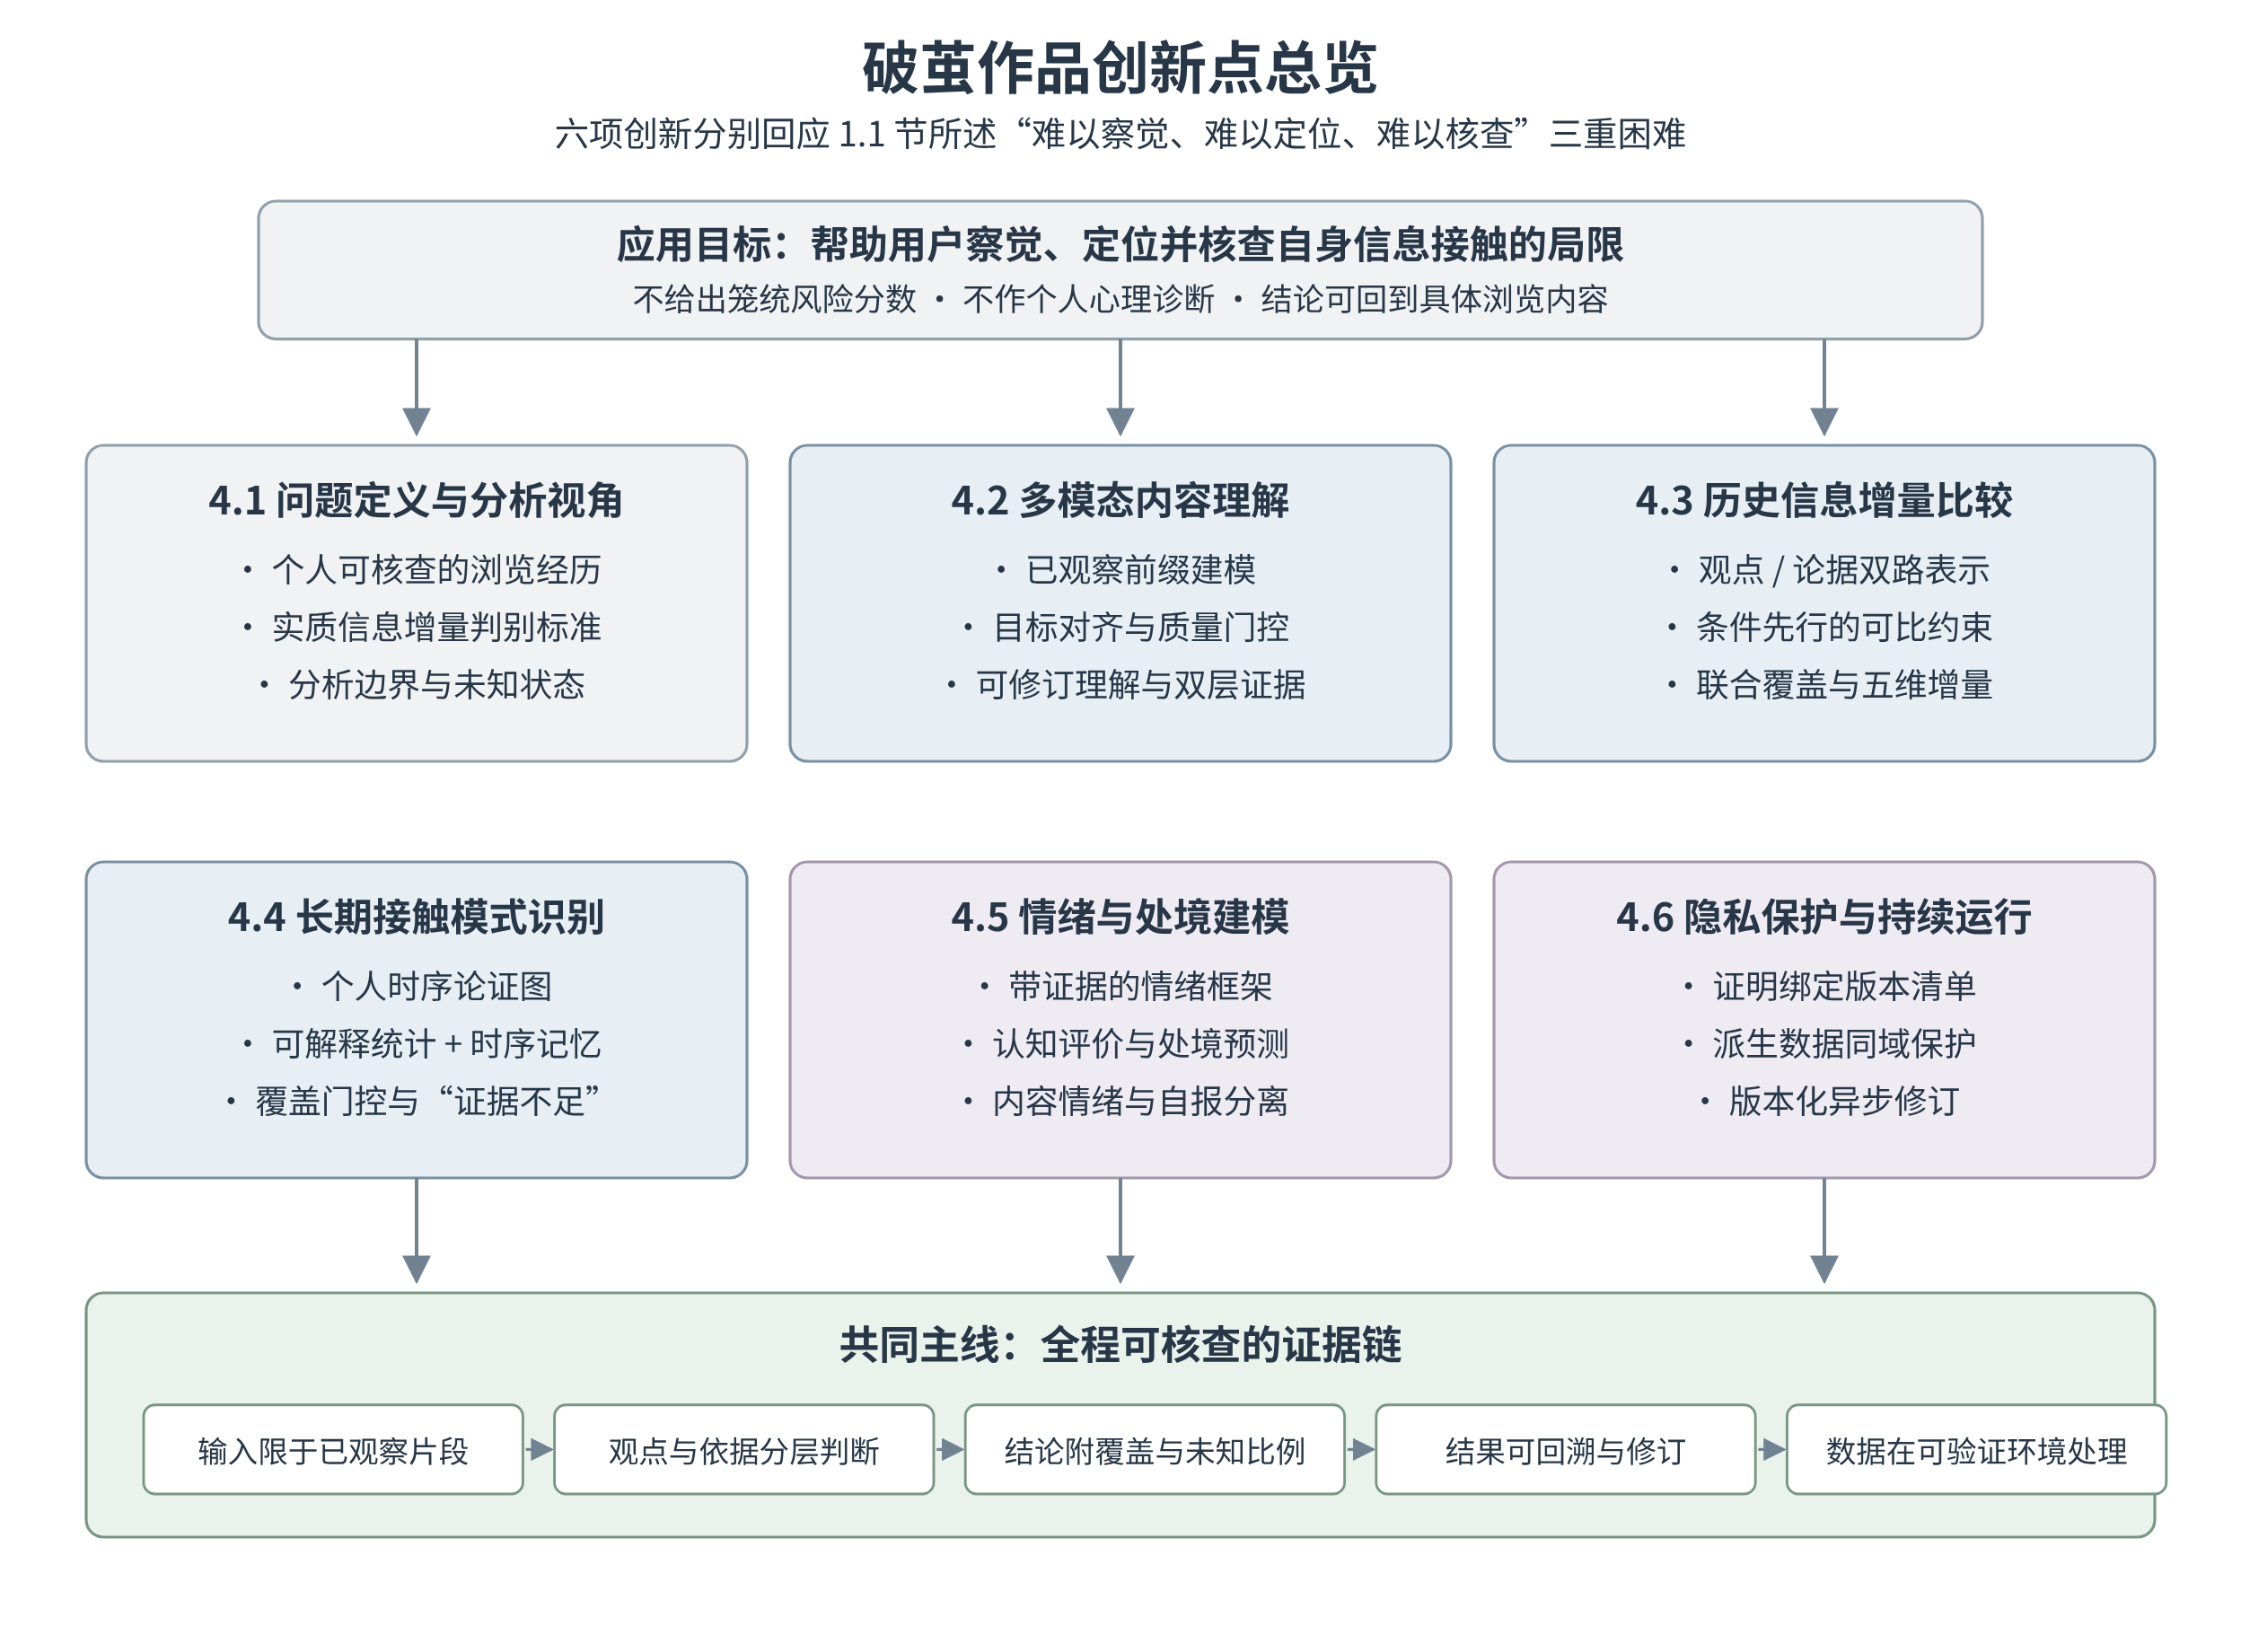
\includegraphics[width=\linewidth,height=0.66\textheight,keepaspectratio]{figures/chapter4/fig_4_1_innovation_overview.png}
\caption{破茧作品创新点总览}\label{fig:4-1}
\end{figure}

六项创新分别回应``难以察觉、难以定位、难以核查''三重困难，并以全程可核查的证据链为共同主线。

表~\ref{tab:4-1} 将上述创新按``现有方案的典型做法---本作品的做法---创新指向的问题''汇总。各项创新分别对应第三章设置的实验对照：内容理解层比较纯文本、模态拼接与完整证据约束方法，并消融对象条件、质量门控与证据监督，部分观察阶段的比较用于评价后续片段到达时的修订效果；历史比较层检验双路表示对``同观点新依据''与``换写旧材料''的区分能力；长期识别层通过去除历史增量、来源关系、时间编码与记忆考察各要素贡献；机密计算层测量证明、传输、推理与提交各阶段的开销及安全用例的实际拦截环节。创新的成立以这些对照结果为依据，不以功能存在本身为据。

\begin{longtable}[]{@{}
  >{\RaggedRight\arraybackslash}p{(\linewidth - 6\tabcolsep) * \real{0.2500}}
  >{\RaggedRight\arraybackslash}p{(\linewidth - 6\tabcolsep) * \real{0.2500}}
  >{\RaggedRight\arraybackslash}p{(\linewidth - 6\tabcolsep) * \real{0.2500}}
  >{\RaggedRight\arraybackslash}p{(\linewidth - 6\tabcolsep) * \real{0.2500}}@{}}
\caption{本作品与现有方案的主要区别}\label{tab:4-1}\tabularnewline
\toprule\noalign{}
层面 & 现有方案的典型做法 & 本作品的做法 & 创新指向的问题 \\
\midrule\noalign{}
\endfirsthead
\toprule\noalign{}
层面 & 现有方案的典型做法 & 本作品的做法 & 创新指向的问题 \\
\midrule\noalign{}
\endhead
\bottomrule\noalign{}
\endlastfoot
分析对象 & 群体传播结构、平台环节或问卷自报\cite{ref1,ref3,ref6}；数字健康工具统计时长\cite{ref2} & 个人授权范围内可核查的浏览经历，结论可回到具体片段 & 茧房难以被个人察觉、定位与核查 \\
判别标准 & 主题占比、观点一致性或文本相似度 & 观点重复、五维实质信息增量与时间持续性三者结合 & 误伤合理的专题阅读，漏判换写式重复 \\
内容理解 & 完整文本的立场或论证抽取\cite{ref8,ref13}，模态齐全的多模态融合\cite{ref14} & 已观察前缀建模、目标条件对齐、质量门控、可修订理解与双层证据记录 & 局部、冲突、快速变化的实际浏览输入 \\
历史比较 & 单一文本相似度或整体语义匹配 & 观点与论据双路表示、条件先行约束、多历史联合覆盖 & 同观点新依据与换写旧材料的混淆 \\
长期评估 & 静态快照、时长统计或黑箱模型评分 & 个人时序论证图，可解释统计与时序记忆双路读出，覆盖门控输出``证据不足'' & 长期模式的识别与可解释兼得 \\
情绪分析 & 笼统正负面分类，或将内容情绪等同用户感受 & 带证据的情绪框架、认知评价与处境联合建模，内容情绪与自报反馈数据流分离 & 焦虑表达的情境化理解与心理诊断误写 \\
隐私保护 & 服务端明文处理，或仅本地简单统计 & 证明绑定版本清单、派生数据同域保护、检查点防回退、删除依赖重放 & 持续认知分析中的明文暴露与状态篡改 \\
持续运行 & 一次性分析或简单缓存 & 事件---输入---模型版本三元组驱动的异步修订与统计更新 & 快速浏览现实与分析正确归属的矛盾 \\
\end{longtable}

\subsection{本章小结}\label{section:4.8}

本章从问题定义、内容理解、历史比较、长期识别、情绪建模、隐私保护与持续运行七个层面说明了作品的创新性。贯穿其中的共同线索是：本作品不追求给出一个更灵敏的茧房分数，而是把分析建立为一条用户可以全程核查的证据链——输入限定于实际观察的片段，判断区分观点与依据两层关系，长期结论附带覆盖与未知状态，结果可以回到原文修订，个人数据在可验证的环境中处理。各项创新分别对应第三章的对照与消融实验，其实际改进幅度以实验结果为准；对用户认知觉察的最终帮助，则留待用户研究检验。

% 第五章正文，直接编辑本文件。
\FloatBarrier\clearpage

\section{总结}\label{chapter:5}

\subsection{工作总结}\label{section:5.1}

本作品针对信息茧房难以被个人察觉、定位和核查的问题，设计并实现了个人认知体检工具``破茧''。系统以手机和浏览器端的增量采集为入口，记录用户实际观察的内容片段与接触过程；在可信执行环境内完成多模态观点与论据联合理解、面向个人历史的信息增量识别和基于时序论证图的长期接触模式分析；结果以小时报告、日报和长期报告呈现，每项结论均可回到具体原文片段核查，用户可对错误归属和采集范围作出更正。

围绕四项研究任务，本报告分别给出了方法设计与实验验证。内容理解方面，已观察前缀建模、目标条件对齐与质量门控使分析范围与用户实际接触保持一致，论证字段 macro-F1 为 0.846，主体归属准确率为 0.934，新增片段到达后结果按版本修订。历史比较方面，观点与论据双路表示配合多历史联合覆盖，Recall@50 为 0.941，五维增量 macro-F1 为 0.837，能够区分``相同观点获得新依据''与``相同观点反复换写''。长期识别方面，时序论证图在用户隔离协议下 macro-F1 为 0.834、ECE 为 0.034，正常专题学习的误报率降至 6.4\%。安全与运行方面，远程证明、密钥分离、检查点防回退与删除重放构成完整的机密计算协议，规定的恶意用例全部被拒绝或隔离，机密执行相对常规执行的分析时延增量为 11.18\%；系统在 10 事件/秒的基础负载下长期稳定运行。

与既有方案相比，作品的差异集中在三处：分析对象限定为个人授权范围内可核查的浏览经历，而非群体结构或问卷自报；判别依据采用观点重复、五维信息增量与时间持续性的组合，而非主题占比或文本相似度；隐私保护覆盖配置一致性、派生数据与历史状态管理，而非仅保护单次推理的输入。上述差异的实际作用均由第三章的对照与消融实验分别检验。

\subsection{不足与适用范围}\label{section:5.2}

系统仍存在明确的边界。采集层在极快切换和平台页面结构变化时仍有误报与漏报，跨应用采集依赖系统能力与目标应用的授权策略；语义层对反讽、多主体同屏和隐含条件的处理不完善，未观察区域的内容不进入分析；长期结论受观察覆盖限制，采集不足的窗口只能输出``证据不足''；情绪与个体反应的一致性基于自愿自报反馈，不构成临床效度，也不证明浏览内容与个人情绪之间的因果关系。

报告的性质是用户审视自身信息环境的材料。系统不将内容相似、观点一致或负面情绪直接作为认知受损的证据，不根据浏览记录推断用户认同或心理状态；对用户信息选择的最终帮助，需要后续用户研究检验。本章所述性能与安全结论均对应第三章规定的硬件、负载与威胁模型，不外推为一般条件。

\subsection{后续研究方向}\label{section:5.3}

后续工作可从三个方向展开。一是用户研究：招募更大规模的参与者，检验认知体检报告是否改善用户对自身信息局限的觉察，以及这种觉察是否转化为信息选择行为的变化。二是方法改进：针对残余误差较集中的反讽识别、隐含条件恢复和长视频部分观察场景扩充训练数据，并探索覆盖不足时更细粒度的拒识策略。三是工程完善：扩展 iOS 与更多浏览器平台的采集适配，降低机密执行在会话建立与状态提交环节的固定开销，并研究多设备并行提交下的协调协议。

\FloatBarrier
\bibliographystyle{gbt7714-numerical}
\bibliography{references}
\cgscLastPage
\end{document}
